%% Based on a TeXnicCenter-Template by Gyorgy SZEIDL.
%%%%%%%%%%%%%%%%%%%%%%%%%%%%%%%%%%%%%%%%%%%%%%%%%%%%%%%%%%%%%

%----------------------------------------------------------
%
\documentclass{book}%
%
%----------------------------------------------------------
% This is a sample document for the standard LaTeX Book Class
% Class options
%       --  Body text point size:
%                        10pt (default), 11pt, 12pt
%       --  Paper size:  letterpaper (8.5x11 inch, default)
%                        a4paper, a5paper, b5paper,
%                        legalpaper, executivepaper
%       --  Orientation (portrait is the default):
%                        landscape
%       --  Printside:   oneside, twoside (default)
%       --  Quality:     final(default), draft
%       --  Title page:  titlepage, notitlepage
%       --  Columns:     onecolumn (default), twocolumn
%       --  Start chapter on left:
%                        openright(no, default), openany
%       --  Equation numbering (equation numbers on right is the default):
%                        leqno
%       --  Displayed equations (centered is the default):
%                        fleqn (flush left)
%       --  Open bibliography style (closed bibliography is the default):
%                        openbib
% For instance the command
%          \documentclass[a4paper,12pt,reqno]{book}
% ensures that the paper size is a4, fonts are typeset at the size 12p
% and the equation numbers are on the right side.
%

%%%%%%%%%%%%%%%%%%%%%%
%% PACKAGES
%%%%%%%%%%%%%%%%%%%%%%
\usepackage{amsmath}
%\usepackage[super,square,comma]{natbib}
\usepackage[twoside,letterpaper,width=6in,height=8in]{geometry}
\usepackage{siunitx} % format units properly
\usepackage{wrapfig}
\usepackage[margin=10pt,font=small,labelfont=bf]{caption} % format captions
\usepackage{booktabs} % nicer tables
\usepackage{subcaption} 
\usepackage{csquotes} % block quotes
\usepackage{tikz}
\usepackage[inline, shortlabels]{enumitem} % inline enumeration
%\usepackage{float}
%\usepackage{appendix}
%\usepackage{chngcntr}
%\usepackage{etoolbox}


\usepackage{graphicx} % packages are used to modify the text and create bling.
\usepackage{textcomp}
\usepackage{gensymb}
\usepackage{natbib}
\usepackage{glossaries}

%\usepackage[usenames]{xcolor}% for commenting in color!
\bibliographystyle{ecology}

\RequirePackage{hyperref} % For hyperlinked cross-references
\hypersetup{
    colorlinks,
    citecolor=blue,
    filecolor=blue,
    linkcolor=blue,
    urlcolor=blue
}

\usepackage{amsmath}%
\usepackage{amsfonts}%
\usepackage{amssymb}%
\usepackage{graphicx}
%----------------------------------------------------------
\newtheorem{theorem}{Theorem}
\newtheorem{acknowledgement}[theorem]{Acknowledgement}
%\newtheorem{algorithm}[theorem]{Algorithm}
%\newtheorem{axiom}[theorem]{Axiom}
%\newtheorem{case}[theorem]{Case}
%\newtheorem{claim}[theorem]{Claim}
%\newtheorem{conclusion}[theorem]{Conclusion}
%\newtheorem{condition}[theorem]{Condition}
%\newtheorem{conjecture}[theorem]{Conjecture}
%\newtheorem{corollary}[theorem]{Corollary}
%\newtheorem{criterion}[theorem]{Criterion}
\newtheorem{definition}[theorem]{Definition}
\newtheorem{example}[theorem]{Example}
\newtheorem{exercise}[theorem]{Exercise}
%\newtheorem{lemma}[theorem]{Lemma}
%\newtheorem{notation}[theorem]{Notation}
\newtheorem{problem}[theorem]{Problem}
%\newtheorem{proposition}[theorem]{Proposition}
\newtheorem{remark}[theorem]{Remark}
\newtheorem{solution}[theorem]{Solution}
\newtheorem{summary}[theorem]{Summary}
\newenvironment{proof}[1][Proof]{\textbf{#1.} }{\ \rule{0.5em}{0.5em}}
%----------------------------------------------------------

\AtBeginEnvironment{subappendices}{%
\chapter*{Appendix}
\addcontentsline{toc}{chapter}{Appendices}
%\counterwithin{figure}{section}
%\counterwithin{table}{section}
}


\graphicspath{{graphics/}}

\title{Environmental Science: East Asia and the World}
\author{EnviroLab Asia Fellows}

\makeatletter
\newcommand{\chapterauthor}[1]{%
  {\parindent0pt\vspace*{-25pt}%
  \linespread{1.1}\large\scshape#1%
  \par\nobreak\vspace*{35pt}}
  \@afterheading%
}
\makeatother

\newcommand{\R}{\mathbb{R}}
\newcommand{\CO}{CO$_2$}

\title{Environmental Science: East Asia and the World}
\author{EnviroLab Asia Fellows}

\makeglossaries

\begin{document}

\frontmatter

\maketitle
\tableofcontents

\chapter*{Preface}

\section{Guiding Principles}

In this project, the EnviroLab Asia fellows have written a textbook that highlights examples of environmental processes that occur along a vertical axis. 

Each student contributes to one theme, composed of two examples that highlight environmental issues of East Asia. However, our goal is not to blame East Asian, but to point to linkages of how a range of globalized economy contribute to these environmental problems. 

In the end, it would be useful for us to acknowledge we have some capacity to address these how these global linkages could be modified to reduce these environmental issues. 

\subsection{Goals}

Processes across horizontal boundaries define many environmental patterns that frame human interactions with the environment. How do humans impact processes that cross these boundaries and how do humans influence these ecosystem interface?

\subsection{Rationale}

\subsection{Activity}

Each group will be composed of two students, that will become experts and teach their classmates on the topic. 

\section{East Asia and the World}







\section{Acknowledgments}

Everyone in the world!





\section{Thoughts for the Contributors}

\subsection{Why Learn \LaTeX?}

\subsection{How to Learn \LaTeX?}

This template will NOT teach you how to use \LaTeX! To accomplish that, we'll rely on some great online resource that you can find on the project page. 

Instead this section of the document is designed to demonstrate how our textbook will look, feel, and ultimately how we contribute to the project.

This document also compiles all of our projects into a single PDF, where each chapter is composed of a input tex file.

\subsection{Noting Your Contribution}

Because this is an ongoing project, you should record your contribution to each chapter -- but also let go of these contributions at some point; Others might revise and their authorship might take some precedence, so you should both invest in the product but also be willing to detach from the final outcome as others contribute. This will feel uncomfortable at times, but please note from the beginning this is a social process and as such subject to negotiation. Please be generous to the authors that laid the foundation and be respectful of those that follow. 

\section{Setting Up Book Project--Type Setting w/ \LaTeX}

\subsection{The Standard Latex Book Class}

Currently, the text is written using the standard book class. However, in 2019, I (Los Huertos) will convert the format to a Tufte book class. 

\subsection{Structuring the Text with Nested Hierarchies}

Contributors divide their contributions into sections and subsections. This format allows a consistent approach to structuring the text and forcing themes to be organized in blocks that can be used to organize the overall text. We use section, subsection, and subsubsection to break up the topic into bite sizes. 

To accomplish this, contributors use the \verb"\section{Section}" command for major sections, and the \verb"\subsection{Subsection}" command for subsections, and a similar approach for subsubsections. 

NOTE: for each nested level, it MUST be followed by the lowest level in the section before a paragraph is started -- in contrast to what is shown above!

NOTE: We may dispense with subsubsections in the future to provide a less blocky structure, but for now they remain useful. 

\subsection{Font Changes}

We can use various methods to alter the typeset: \emph{Emphasize}, \textbf{Bold}, \textit{Italics}, and \textsl{Slanted}. We can also typeset \textrm{Roman}, \textsf{Sans Serif}, \textsc{Small Caps}, and \texttt{Typewriter} texts.  Look online to see the commands to accomplish these changes. 

You can also apply the special, mathematics only commands $\mathbb{BLACKBOARD}$
$\mathbb{BOLD}$, $\mathcal{CALLIGRAPHIC}$, and $\mathfrak{fraktur}$. Note that
blackboard bold and calligraphic are correct only when applied to uppercase letters A
through Z.

You can apply the size tags -- Format menu, Font size submenu -- {\tiny tiny},
{\scriptsize scriptsize}, {\footnotesize footnotesize}, {\small small}, {\normalsize
normalsize}, {\large large}, {\Large Large}, {\LARGE LARGE}, {\huge huge} and {\Huge
Huge}.

You can use the \verb"\begin{quote} etc. \end{quote}" environment for typesetting
short quotations. Select the text then click on Insert, Quotations, Short Quotations:

\begin{quote}
The buck stops here. \emph{Harry Truman}

Ask not what your country can do for you; ask what you can do for your
country. \emph{John F Kennedy}

I am not a crook. \emph{Richard Nixon}

I did not have sexual relations with that woman, Miss Lewinsky. \emph{Bill Clinton}
\end{quote}

The Quotation environment is used for quotations of more than one paragraph. Following
is the beginning of \emph{The Jungle Books} by Rudyard Kipling. (You should select
the text first then click on Insert, Quotations, Quotation):

\begin{quotation}
It was seven o'clock of a very warm evening in the Seeonee Hills when Father Wolf woke
up from his day's rest, scratched himself, yawned  and spread out his paws one after
the other to get rid of sleepy feeling in their tips. Mother Wolf lay with her big gray
nose dropped across her four tumbling, squealing cubs, and the moon shone into the
mouth of the cave where they all lived. ``\emph{Augrh}'' said Father Wolf, ``it is time
to hunt again.'' And he was going to spring down hill when a little shadow with a bushy
tail crossed the threshold and whined: ``Good luck go with you, O Chief of the Wolves;
and good luck and strong white teeth go with the noble children, that they may never
forget the hungry in this world.''

It was the jackal---Tabaqui the Dish-licker---and the wolves of India despise Tabaqui
because he runs about making mischief, and telling tales, and eating rags and pieces of
leather from the village rubbish-heaps. But they are afraid of him too, because
Tabaqui, more than any one else in the jungle, is apt to go mad, and then he forgets
that he was afraid of anyone, and runs through the forest biting everything in his way.
\end{quotation}

Use the Verbatim environment if you want \LaTeX\ to preserve spacing, perhaps when
including a fragment from a program such as:
\begin{verbatim}
#include <iostream>         // < > is used for standard libraries.
void main(void)             // ''main'' method always called first.
{
 cout << ''This is a message.'';
                            // Send to output stream.
}
\end{verbatim}
(After selecting the text click on Insert, Code Environments, Code.)


\subsection{Mathematics and Text}

\subsubsection{Warning: Special Characters}

When you use percent and ampersand symbols, hash tags, and other non-standard ASCII characters, \LaTeX will be very uncooperative. So, do yourself a favor and make sure you understand that these are used for special typesetting functions. To use them you have to ``escape'' and use commands to get them to do what you might usually expect!  \% \# \& \`e \~n `` and '' to show a few that do not reflect the key stroke you might expect. 

\LaTeX doesn't like a range of characters or they reserved for special behavior...

For example, the \# is used for tabs in a table environment. \% is used to make comments, thus stuff behind a \% is ignored. There are lots of others, but these come up the most.

\subsubsection{Creating equations}

One of the most powerful parts of \LaTeX is how it can be used to write complex equations, with all those symbols and Greek letters! This can be done inline $y = mx + b + \epsilon$ for fairly simple equations, or set apart for more complex equations:

\begin{equation}
\int_0^\infty e^{-x^2} dx=\frac{\sqrt{\pi}}{2}
\end{equation}

\subsubsection{Theorems, etc}
\begin{theorem}
(The Currant minimax principle.) Let $T$ be completely continuous selfadjoint operator
in a Hilbert space $H$. Let $n$ be an arbitrary integer and let $u_1,\ldots,u_{n-1}$ be
an arbitrary system of $n-1$ linearly independent elements of $H$. Denote
\begin{equation}
\max_{\substack{v\in H, v\neq
0\\(v,u_1)=0,\ldots,(v,u_n)=0}}\frac{(Tv,v)}{(v,v)}=m(u_1,\ldots, u_{n-1})
\label{eqn10}
\end{equation}
Then the $n$-th eigenvalue of $T$ is equal to the minimum of these maxima, when
minimizing over all linearly independent systems $u_1,\ldots u_{n-1}$ in $H$,
\begin{equation}
\mu_n = \min_{\substack{u_1,\ldots, u_{n-1}\in H}} m(u_1,\ldots, u_{n-1}) \label{eqn20}
\end{equation}
\end{theorem}
The above equations are automatically numbered as equation (\ref{eqn10}) and
(\ref{eqn20}).


\subsection{Lists Environments: Making bulletted, numbered, description lists}

We use special commands to create an itemized list.

You can create numbered, bulleted, and description lists
(Use the Itemization or Enumeration buttons, or click on the Insert menu
then chose an item from the Enumeration submenu):

\begin{enumerate}
\item List item 1

\item List item 2

\begin{enumerate}
\item A list item under a list item.

\item Just another list item under a list item.

\begin{enumerate}
\item Third level list item under a list item.

\begin{enumerate}
\item Fourth and final level of list items allowed.
\end{enumerate}
\end{enumerate}
\end{enumerate}
\end{enumerate}

\begin{itemize}
\item Bullet item 1

\item Bullet item 2

\begin{itemize}
\item Second level bullet item.

\begin{itemize}
\item Third level bullet item.

\begin{itemize}
\item Fourth (and final) level bullet item.
\end{itemize}
\end{itemize}
\end{itemize}
\end{itemize}

\begin{description}
\item[Description List] Each description list item has a term followed by the
description of that term.

\item[Bunyip] Mythical beast of Australian Aboriginal legends.
\end{description}

\subsection{Theorem-Like Environments}

The following theorem-like environments (in alphabetical order) are available
in this style.

%\begin{acknowledgement}
%This is an acknowledgement
%\end{acknowledgement}

%\begin{algorithm}
%This is an algorithm
%\end{algorithm}

%\begin{axiom}
%This is an axiom
%\end{axiom}

%\begin{case}
%This is a case
%\end{case}

%\begin{claim}
%This is a claim
%\end{claim}

%\begin{conclusion}
%This is a conclusion
%\end{conclusion}

%\begin{condition}
%This is a condition
%\end{condition}

%\begin{conjecture}
%This is a conjecture
%\end{conjecture}

%\begin{corollary}
%This is a corollary
%\end{corollary}

%\begin{criterion}
%This is a criterion
%\end{criterion}





\begin{example}
This is an example
\end{example}

\begin{exercise}
This is an exercise
\end{exercise}

%\begin{lemma}
%This is a lemma
%\end{lemma}

%\begin{proof}
%This is the proof of the lemma.
%\end{proof}

%\begin{notation}
%This is notation
%\end{notation}

%\begin{problem}
%This is a problem
%\end{problem}

%\begin{proposition}
%This is a proposition
%\end{proposition}

%\begin{remark}
%This is a remark
%\end{remark}

%\begin{summary}
%This is a summary
%\end{summary}

%\begin{theorem}
%This is a theorem
%\end{theorem}

%\begin{proof}
%[Proof of the Main Theorem]This is the proof.
%\end{proof}

%\subsubsection{``Child'' Rnw Contributions}

%This is a chapter that we can input into the text... you will each create a chapter without the preamble and begin and end document... that can be integrated into a single book! 

\subsection{Peer Review Commenting}

You can put your comments in square brackets and in color for things that need help. \textcolor{red}{[This section is confusing, I am not sure what commenting means.]}

\subsection{Adding Figures, etc}

\subsection{Using Rnw Files -- Deprecated}

Originally, I used R and Rnw files that were converted to tex files, in Rstudio. However, this step was too complicated for students, so I now recommend the use of tex files and use Rstudio to create figure files as a separate process. Thus, I will no longer explain the process in this document. 

\subsection{Creating a floating figure}

This is my floating figure (Figure \ref{fig:plot}).

\begin{figure}

\caption{My plot's caption is here!}
\label{fig:plot}
\end{figure}

\subsection{Using Boxes}

\fbox{
\begin{minipage}[c]{.9\textwidth}
\subsection{minibox X}

Some text
\end{minipage}
}

\subsection{Creating References, Indicies, and Glossaries}

\subsubsection{Bibliography generation}

This document was produced in RStudio using the knitr package \citep{knitr2013} by \url{http://texblog.org}. 

Also try \citet{fenner2018} to create an author title. 

Currently, we are using the ecology.bst, but it has trouble with misc type of references, so I will changing this in 2019. 

\subsubsection{Creating glossary words}
 
\newglossaryentry{peat}{
	name=Peat, 
	description={peat is cool.}
}

\begin{definition}
This is a definition and the word is use in an glossary, e.g. \gls{peat}. \Gls{peat} is when you want to capitalize the defined word without having to re-define a capitalized version, the only downside of case sensitivity in \LaTeX.
\end{definition}
\input{chapters/001_Introduction}

\mainmatter
\part{Vertical Processes}

%%%%%%%%%%%%%%%%%%%%%%%%%%%%%%%
%%  CHAPTERS BY FELLOWS AND FACULTY 
%%%%%%%%%%%%%%%%%%%%%%%%%%%%%%%%
%%%%%%%%%%%%%%%%%%%%%%%%%%%%%%%
%%  INTRO AND MOTIVATION 
%%%%%%%%%%%%%%%%%%%%%%%%%%%%%%%

\chapter{The Earth-Sun System: Atmospheric Composition and Energy Balance}\label{ch:earth_sun} 
\chapterauthor{Colin Adams\footnote{Colin Adams completed all the research, writing, and developed the graphics for this chapter.}}

\section{\label{sec:pbd}The Pale Blue Dot}

\subsection{Voyager 1's Legacy}

On September 5, 1977, the \emph{Voyager 1} space probe was launched into space by the United States' National Aeronautics and Space Administration (NASA). The space probe's mission was to explore the outer solar system, specifically, to study Jupiter and Saturn. In 1990, after completing its original purpose,  \emph{Voyager 1} received a new mission: take a solar system ``family portrait.'' That is, from a distance of approximately 6 billion kilometers from the sun, \emph{Voyager 1} would take pictures of six planets and their relative positions by combining different images together.

On February 14, 1990  \emph{Voyager 1} turned around and pointed its camera back at Earth. It took 60 different photos of the solar system (see Figure~\ref{fig:EarthSunVenus}) and sent them back to Earth where they were stitched together. It took over five and a half hours to transmit the photographic data across the vast expanse of space, from \emph{Voyager 1} back to Earth. 

    \begin{figure}[ht]
    \centering
		\includegraphics[width=0.55\textwidth]{SunEarthVenus_PBD.png}
		\caption{A picture of the sun and inner solar system. Superimposed on the left side are pictures of Venus and Earth (see Figure~\ref{fig:pale_blue_dot}). This is what \emph{Voyager 1} saw nearly 6 billion \si{\km} away from the sun. Image taken from NASA/JPL.}
        \label{fig:EarthSunVenus}
    \end{figure}

Three of the sixty photographs contained Earth as a single point of light. By processing these three photographs, NASA was able to produce an image of the earth taken over six billion kilometers away from the sun. In each case, Earth was less than a single pixel in each of the photographs %\citep{planetary}.

    \begin{figure}[ht]
    \centering
\includegraphics[width=0.70\textwidth]{PaleBlueDot.jpg}

        \caption{The Pale Blue Dot. This is perhaps the most famous photograph taken by \emph{Voyager 1} on February 14, 1990. The the size of the Earth is less than a single pixel. The Earth is circled for clarity. Image taken and modified from NASA/JPL.}
        \label{fig:pale_blue_dot}
    \end{figure}

    Coincidentally, when the photograph was taken, sunlight scattered across the lens of the camera, creating the illusion that the earth was caught in a ray of light from the sun (see  Figure~\ref{fig:pale_blue_dot}). In his book, astronomer Carl Sagan commented upon this image and its significance:
    \begin{displayquote}
        \small %change font size to distinguish quote from rest of text
        \quad Look again at that dot. That's here. That's home. That's us. On it everyone you love, everyone you know, everyone you ever heard of, every human being who ever was, lived out their lives. The aggregate of our joy and suffering, thousands of confident religions, ideologies, and economic doctrines, every hunter and forager, every hero and coward, every creator and destroyer of civilization, every king and peasant, every young couple in love, every mother and father, hopeful child, inventor and explorer, every teacher of morals, every corrupt politician, every ``superstar,'' every ``supreme leader," every saint and sinner in the history of our species lived there---on a mote of dust suspended in a sunbeam.

        \quad The Earth is a very small stage in a vast cosmic arena. Think of the rivers of blood spilled by all those generals and emperors so that, in glory and triumph, they could become the momentary masters of a fraction of a dot. Think of the endless cruelties visited by the inhabitants of one corner of this pixel on the scarcely distinguishable inhabitants of some other corner, how frequent their misunderstandings, how eager they are to kill one another, how fervent their hatreds.

        \quad Our posturings, our imagined self-importance, the delusion that we have some privileged position in the Universe, are challenged by this point of pale light. Our planet is a lonely speck in the great enveloping cosmic dark. In our obscurity, in all this vastness, there is no hint that help will come from elsewhere to save us from ourselves.

        \quad The Earth is the only world known so far to harbor life. There is nowhere else, at least in the near future, to which our species could migrate. Visit, yes. Settle, not yet. Like it or not, for the moment the Earth is where we make our stand.

        \quad It has been said that astronomy is a humbling and character-building experience. There is perhaps no better demonstration of the folly of human conceits than this distant image of our tiny world. To me, it underscores our responsibility to deal more kindly with one another, and to preserve and cherish the pale blue dot, the only home we've ever known \cite{sagan}.
    \end{displayquote}

    With this perspective, we delve into the study of the earth, its environment, and us. We attempt to unearth our interactions with and our impacts on our only home. To begin, we look at the interaction between the earth and its main source of energy: the sun. By doing this, we will understand the greenhouse effect and its necessity by looking at very crude models of the earth and its atmosphere. 

    %%%%%%%%%%%%%%%%%%%%%%%
    %% FORMATION OF SS
    %%%%%%%%%%%%%%%%%%%%%%%

    \section{\label{sec:solar_sys}Formation of the Solar System}
		
		\subsection{The Nebular Hypothesis}

    Nobody is entirely sure how the solar system formed, but there are a few \textbf{hypotheses} on how it did. Here, we will present the Nebular hypothesis of its formation.


\newglossaryentry{nebulae}{
	name=Nebulae, 
	description={huge clouds of gas.}
}
    As we know it today, the solar system is anywhere from 4.5 to 4.8 billion years old. Scientists believe stars form from huge clouds of gas (called a \gls{nebulae}) and other, heavier elements. The gas is compressed by gravity, becoming more and more dense until the gas gets so hot that two protons combine to form helium. %\footnote{
        % This is not the complete picture. If p is a proton, d is deuterium (a proton and neutron binded together), e$^+$ is a positron (anti-electron), $\nu_e$ is a neutrino, and $\gamma$ is a high energy photon, then the actual reaction looks something like:
        % \begin{align*}
        % \text{p} + \text{p} &\to \text{d} + \text{e}^{+} + \nu_e + \SI{0.4}{\mega \electronvolt}\\
        %   \text{d} + \text{p} &\to {}^3\text{He} + \gamma + \SI{5.5 }{\mega \electronvolt} \\
        %   {}^{3}\text{He} + {}^3\text{He} &\to {}^4\text{He} + \text{p} + \text{p} +  \SI{12.9}{\mega \electronvolt}
        % \end{align*}
        % If we add two of the first and second reaction to one of the third reaction we get the overall reaction of
        %     \[
        %     4 \text{p} \to {}^4\text{He} + 2\text{e}^{+} + 2\nu_e + \SI{24.7}{\mega \electronvolt}
        %     \]
        % which effectively turns hydrogen into helium; N.B.: \SI{1}{\electronvolt} = \SI{1.602e-19 }{\joule}. This is not crucial for developing a good understanding and can be skipped, however I leave it here for the interested reader \citep{thorndike1976energy,townsend2010baby}}
    This process is known as \textbf{nuclear fusion}. When fusion occurs, the star releases a tremendous amount of energy in the form of electromagnetic radiation---such as visible light, infrared light (IR), x-rays, ultraviolet (UV) rays, radio waves, etc.---and the ball of gas begins to shine. When this happens, a star is born. Like every star, the sun was formed after the gravitational collapse of a nebula. This process occurred over the course of about a million years \citep{formation_solar}.

    In the process of this formation, a disk of gas and other elements caught by the sun's immense gravitational pull began to clump together to form grains that collided into one another, becoming bigger, and bigger. Over the course of 10--100 million years, these grains collided and merged until they became large enough to form the planets of our solar system \citep{hayashi1985formation}.

\subsection{Rocky versus Giant Gas Planets}

    The \textbf{terrestrial planets}, also known as the rocky planets, (e.g. Mercury, Venus, Earth, and Mars) are closest to the sun because the inner solar system was too warm to for volatile molecules to be structurally important for the planet. Thus, only elements with higher melting points (iron, nickel, silicon, etc.) could remain in this region. When the planets got large enough, the terrestrial planets' gravity was strong enough to maintain an atmosphere. Unsurprisingly, the more massive a planet is (i.e. the stronger its gravity) the more equipped it is at maintaining its atmosphere. For example, studies have shown that Mars had a much thicker atmosphere with a different composition in the past than it does today, more similar to Earth's. However, Mars has about $1/10$ the mass that Earth does. Current hypotheses believe that solar wind destroyed much of Mars' atmosphere, as it's gravitational field was unable to maintain it while Earth's remained intact despite being closer to the sun \citep{owen1992composition}. Much of the remaining gas of the nebula formed into the much larger \textbf{gas giants} in the outer solar system (Jupiter, Saturn, Uranus, and Neptune) or was blown away by solar wind \citep{hayashi1985formation}.

    Over the next few billion years, the solar system evolved into what we see today. At some point along the way, water formed on the surface of the earth and life soon followed---exactly how remains one of the great mysteries of modern science. Over billions of years, life evolved into what we see around us today \citep{bell2015potentially} As life enveloped the earth's surface, spreading to every corner, it changed everything from its the physical surface to the composition of the atmosphere.

    %%%%%%%%%%%%%%%%%%%%%%%%%%%%%%%%%%%
    %%   ENERGY TRANSFER B/W E+S
    %%%%%%%%%%%%%%%%%%%%%%%%%%%%%%%%%%%

    \section{\label{sec:energy_flow}Global Energy Flow}
		
\subsection{Radiant Energy Impinges on the Earth's Atmosphere}

    The earth's principal source of energy comes from the sun which releases radiant energy that impinges upon the earth's atmosphere.  Some of this energy is reflected back into space by clouds, some is absorbed by the clouds themselves, while some penetrates through the atmosphere making it to the earth's surface, where it is again either reflected or absorbed. Some of the energy is indeed reflected (water, snow, ice, clouds---in what is known as the \textbf{albedo effect}). Once it makes it to the earth's surface, it is absorbed and \emph{re-radiated}.

    When this energy is absorbed by the surface, it warms the soil or water. The warmer soil and water can transfer energy from the surface to the lower atmosphere by \textbf{conduction}. The warmer, lower atmosphere transfers energy horizontally and vertically of the upper atmosphere layers through \textbf{convection}.\footnote{
        Conduction is the direct transfer of heat or electricity without the movement of the material. Convection is the transfer of heat through the movement caused within a fluid. A good example to keep the two straight in your head would be a wood-fired furnace. When you touch the furnace (and probably burn your hand), you are warming your hand through direction contact with a material, i.e. conduction. When you place your hand just above the furnace (the safer thing to do), you are letting the air (a fluid) warm your hand through by first warming the surrounding air that is transfered to your hand, i.e. convection.
        } 
				
    In addition to all of this, the atmosphere can lose some of this heat by re-radiating some of this energy in the form of infrared light. This infrared light can either be sent back to the earth's surface, ejected into space, or re-absorbed somewhere else in the atmosphere. Eventually, the vast majority of the energy that has entered near the earth will leave it. 

    If this process seems like a complicated, then you are correct! What was described above is what ultimately determines the earth's temperature, climate, and weather.
		
\subsection{Energy is Conserved}

    Because energy is always conserved and there is negligible energy that is gained by the earth, there is a balance between the amount of energy the earth receives from the sun and the amount it radiates away over a given period of time. In other words, the earth and the sun are in \textbf{equilibrium} with each other \citep{thorndike1976energy}. If they were not, the earth would continue to get warmer and warmer over time until it was in equilibrium with the sun. However, when considering the whole surface of the earth, the surface temperature is essentially constant implying an equilibrium. To emphasize this point once more, the earth radiates away energy at the same rate it receives it from the sun. This will be the fundamental basis for the rest of the chapter where we will use very simple models in order to gain a better understanding of the earth, its atmosphere, and the greenhouse effect.


        \subsection{The Sun and the Solar Constant} % (fold)
        \label{sub:the_sun}
        
        The sun is approximately \SI{1.5e8}{\km} away from the earth with a surface temperature of about \SI{5800}{\kelvin}. By simply knowing the temperature of the sun's surface as well as its distance away from the earth, we are able to calculate the frequency distribution of the light emitted by the sun (Figure~\ref{fig:sun_bb}) as well as its brightness. This is because, to a very good approximation, the sun (and the earth, as we will later see) behaves as a blackbody which emits \textbf{blackbody radiation}. You probably are familiar with the idea of blackbody radiation whether you know it or not. When an object is at a certain temperature, it emits light centered around a peak wavelength and other wavelengths of light are distributed about this peak. The distributions of emitted light from objects at different temperatures have similar shapes but have their peak wavelength value at a different value. The hotter the object, the shorter its wavelength and the bluer it looks. This is why hot objects glow red, hotter objects glow blue, and even hotter objects glow white. We can treat both the sun and the earth as objects at a certain temperature. The sun mostly emits visible light while the earth emits infrared light (See Figure~\ref{fig:sun_bb} and Figure~\ref{fig:earth_bb} for a visual representation of this).

        The surface temperature of the sun as well as its distance from Earth is enough information to calculate a value called the \textbf{solar constant}, which we will denote by $\mathcal{S}$ in this text. The solar constant tells us the amount of solar energy per unit time and per unit area the earth receives. The units are \si{\joule/\second/\meter^{2}} = \si{\watt/\meter^{2}}. A joule, denoted by \si{\joule}, is a unit of energy. For a concrete example, an object that has a mass of \SI{2}{\kg} that is moving at \SI{1}{\m/\s} has one joule of energy. The amount of energy released during a given period of time is a measure of power. Here we use watts as the unit of power, which is denoted by \si{\watt}, and is defined to be $\SI{1}{\watt} = \SI{1}{\joule/\s}$. 

        One way to visualize what the solar constant actually means is to imagine a unit of area (in this case, one square meter) that is placed just above the earth's atmosphere oriented such that the sun shines squarely on it. The amount of energy (measured in joules) that flows through that area in a given amount of time (in this case, one second). This solar constant has been measured to be $\mathcal{S} = \SI{1370}{\watt/\m^2}$ \citep{schroeder1999introduction,thorndike1976energy}p
        % subsubsection the_sun (end)

        \begin{figure}[ht]
            \centering
            \includegraphics[width = 0.8\textwidth]{sun_blackbody.pdf}
            \caption{The intensity of light as a function of wavelength for an object the same temperature as our Sun (\SI{5800}{\kelvin}). This distribution of wavelengths is only dependent on the temperature of the object. The black portions of the distribution are wavelengths of light that human eyes cannot detect. Looking at this, you should realize that it is no coincidence that life on Earth managed to evolve to see in the visible spectrum of light.}
            \label{fig:sun_bb}
        \end{figure}

        We have already discussed that the earth and the sun are in equilibrium with one another. Again, this simply means that the earth is radiating the same amount of energy into space as it receives from the sun in a given period of time. The total power (energy per unit time) that is emitted by an object is given by
        \begin{equation}
            \text{power} = \sigma e A T^4
            \label{eq:stefan_law}
        \end{equation}
        where $T$ is the object's temperature, $A$ is the object's area, $e$ is the object's emissivity,\footnote
        {
            The emissivity is the fraction of light absorbed at a particular wavelength. For an object that absorbs all incoming light (a blackbody) then $e = 1$; an object that reflects all light would have $e = 0$.
        } 
        and $\sigma$ is the Stefan-Boltzmann constant\footnote
        {
            This is just a constant (with units!), and is rather easy to remember. Just think ``5-6-7-8'' but don't forget the minus sign in front of the 8.
        } 
        where 
        \begin{equation}
            \sigma = \SI[per-mode=fraction]{5.67e-8}{\watt \per (\meter^2  \kelvin^4)}. 
        \end{equation}
        Equation~(\ref{eq:stefan_law}) is known as \textbf{Stefan's Law}. An important point: when using Eq.~(\ref{eq:stefan_law}), you must be careful to use the correct temperature units of Kelvin. To convert between Celsius and Kelvin we have a conversion formula of $T_K = T_C + 273.15$ where $T_K$ is the temperature in Kelvin and $T_C$ is the temperature in Celsius.

        \begin{exercise}
            What is the temperatures of water's
            \begin{enumerate*}[(a)]
                \item  freezing point (\SI{0}{\celsius})
                \item and boiling point at sea level (\SI{100}{\celsius})
                given in kelvin?
            \end{enumerate*}
        \label{ex:kelvin}
        \end{exercise}

        \begin{exercise}
        If a person's body has a surface area of roughly \SI{1.4}{\meter^2} and a  temperature of \SI{37}{\celsius} (take $e = 1$):
            \begin{enumerate}[(a)]
                \item How much power does a person give off? 
                \item Compare the total \underline{energy} radiated by your body in one day compared to the energy in the food that you eat. Why is there such a large discrepancy? (Note that $\SI{1}{\text{Calorie}}=\SI{4184}{\joule}$).
            \end{enumerate}
            \label{ex:humans}
        \end{exercise}

    \subsection{The Dark Earth Model} % (fold)
    \label{sub:dark_earth}

    Now we are finally able to model the energy flow to and from the earth. However, the ``earth'' that we will first be describing will be a rather simple one: it will have no atmosphere and no oceans. We will also assume that this earth is a perfect blackbody (with $e =1$), meaning that it reflects \emph{no} incident radiation from the sun. Previously, we argued that earth was in equilibrium with the sun. Again, the rate at which the earth receives energy from the sun is the same as the rate the earth expels energy. So if we balance the amount of energy flowing from the sun to the earth over a given period of time, ($\mathcal{S}$), and set it equal to the amount of energy being emitted by the earth over a given period of time, we can calculate the surface temperature of the earth. That is, we have
    \begin{align}
        \mathcal{S}\underbrace{(\pi R^2)}_{A_{circ}} = \underbrace{(4\pi R^2)}_{A_{sph}} \sigma T^4
        \label{eq:earth_balance}
    \end{align}
    where $R$ is the radius of the earth and $T$ is the surface temperature of the earth. Now each term contained within parentheses of Eq.~(\ref{eq:earth_balance}) is the relevant area. On the left-hand side of the equation, the sun only sees the earth as a circular disk, hence we use the area of a circle $A_{circ} = \pi r^2$. However, the earth emits this radiation from all directions of a sphere, which---you may remember from geometry---has a surface area of $A_{sph} = 4 \pi r^2$. When we solve for the temperature, $T$, in Eq.~(\ref{eq:earth_balance}) we get 
    \begin{align}
        T = \left( \frac{\mathcal{S}}{4 \sigma} \right)^{1/4} = \left( \frac{\SI{1370}{\watt/\meter^2}}{4 \cdot \SI{5.67e-8}{\watt/(\meter^2 \kelvin^4)} } \right)^{1/4} = \SI{279}{\kelvin}
        \label{eq:earth_temp}
    \end{align}
    which is actually a really good estimate for the earth's equilibrium temperature because the average surface temperature is measured to be \SI{288}{\kelvin} (\SI{15}{\celsius}) \citep{schroeder1999introduction} In fact, this simple model agrees too well! We had no right to be this close to what we measure with the crudeness of our assumptions. This will become apparent when we refine the model in Sec.~\ref{sub:shiny_earth}. However, before moving on to a better model, we should discuss the stability of the earth-sun system by discussing the concept of \textbf{feedback}---a process in which a system reacts to an action or behavior.


%\begin{fbox}
%\begin{minipage}{5in}

\subsubsection{Feedback---A Digression} % (fold)
		\textcolor{red}{[LET'S MAKE THIS INTO A TEXT BOX -- PROBABLY USING MINIPAGE FUNCTIONS.]}
    \label{ssub:feedback}
    Feedback loops crop up all over the natural world and are especially prominent when studying the environment. Because of this, being able to recognize and identify various feedback loops is an important skill to have.
    
    Consider three balls placed on three different surfaces: one on a concave surface, one on a flat surface, and one on a convex surface as illustrated in Figure~\ref{fig:feedback}. When placed on the surfaces at rest and left undisturbed, the three balls will remain at rest forever; however, if the balls are slightly bumped then there are three very different responses. 

    The concave ball (the leftmost) will try to return back to its starting location if displaced. This is known as a \textbf{stable equilibrium}. The initial displacement leads the ball to feel a restoring force pushing it back to where it started. The restoring force in this case would be gravity, and it is said to provide \textbf{negative feedback}. For the ball in the center, we have a situation of \textbf{neutral equilibrium}. If displaced it, it will simply have changed locations but will not return or roll away from its original position. There is \textbf{no feedback} in this situation. Lastly, for a ball on a convex surface (an \textbf{unstable equilibrium}), if it is nudged slightly, the ball will experience a force forcing it away from its equilibrium. As you may have guessed, this is an example of \textbf{positive feedback}. The adjectives of ``positive'' and ``negative'' are not meant to convey ``good'' or ``bad,'' rather they express the direction the system will move towards after being displaced: ``positive'' means move away from where it started whereas ``negative'' means returning to where it started.

    \begin{figure}%[ht]
		\centering
    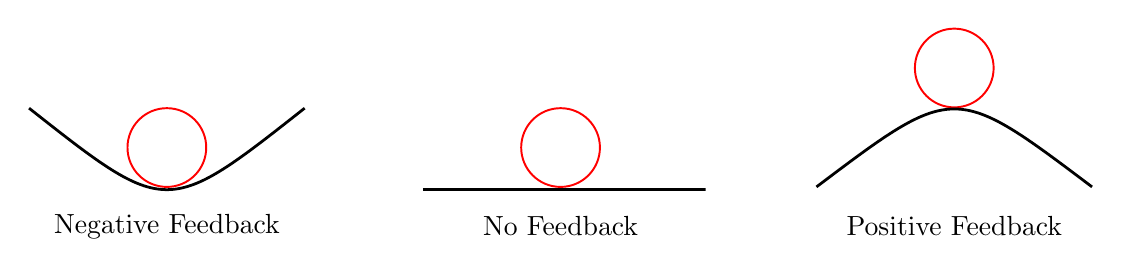
\begin{tikzpicture}%[scale = 1]
        %%%%%%%%% ball in bowl %%%%%%%%%%%%%%%%%
        \draw[color = red, line width = 0.7pt] (0,0) circle(0.5);
        \draw[line width=1.pt] (-1.75, 0.5) .. controls(0,-0.88) .. (1.75, 0.5);  
        \node at (0, -1.0) {Negative Feedback};
        %%%%%%%%% flat plane ball %%%%%%%%%%%%%%  
        \draw[color = red, line width = 0.7pt] (5+0,0) circle(0.5);
        \draw[line width=1.pt] (5-1.75, -0.53) .. controls(5+2,-0.53) .. (5+1.75, -0.53);
        \node at (5, -1.0) {No Feedback};
        %%%%%%%%%% ball on bowl %%%%%%%%%%%%%%%%%
        \draw[color = red, line width = 0.7pt] (10,1.01) circle(0.5);
        \draw[line width=1.pt] (10-1.75, -0.5) .. controls(10,0.82) .. (10+1.75, -0.5);
        \node at (10, -1.0) {Positive Feedback};
    \end{tikzpicture}   
    \caption{An example of various feedback loops. Consider a ball at rest on various surfaces that is suddenly displaced by a small amount in one direction (we are looking at a cross section). On the left, a ball is in a bowl, and when displaced from either side, the ball will roll back and forth, always returning to the center of the bowl. In the middle image, we have a ball on a flat surface. When displaced, it simply changes locations. On the right, we have a ball balanced on a bowl. If displaced slightly, its balance is upset, and it will roll down the bowl faster and faster and faster.}
    \label{fig:feedback}
    \end{figure}

    This may have been a lengthy aside but one that is important. For example, if we look at feedback in the context of our dark earth model, then we need to consider a few situations. For instance, consider what would happen if the surface temperature drops to below its equilibrium temperature. According to Stefan's Law (Eq.~\ref{eq:stefan_law}), then the rate at which the earth energy would be radiated away would also drop, cooling itself, thus returning to equilibrium. This is an example of negative feedback.

    \begin{exercise}
        Find two examples of feedback loops on your own: one positive and one negative.
        \label{ex:feedback_loops}
    \end{exercise}

    % subsubsection feedback (end)

%\end{minipage}
%\end{fbox}

    \subsection{The Shiny Earth Model} % (fold)
    \label{sub:shiny_earth}
   
    To motivate why we need to refine our model of the earth, we should consider Figure~\ref{fig:earthrise}.

    \begin{figure}[hb!]
        \centering
        \includegraphics[width = 0.6\textwidth]{earthrise.jpg}
        \caption{The famous ``Earthrise'' photo taken during the Apollo 8 lunar mission. Image taken from NASA.}
        \label{fig:earthrise}
    \end{figure}

    If the earth, as we assumed in Sec.~\ref{sub:dark_earth}, absorbed all incident light, we would not see an image like the Apollo 8 astronauts did; rather we would see nothing as the earth would appear black.  From our everyday experience, we know some objects (e.g. clouds, ice, snow, etc.) reflect a large fraction of the light incident upon them (see Table~\ref{tab:albedo}), again illustrated in Figure~\ref{fig:earthrise}. The reflectivity of an object averaged over the entire surface is known as its \textbf{albedo}, and we will denote it as $A$ in equations in this text. The earth reflects roughly 30\% of the sun's incident light, meaning that $A = 0.30$, and the remaining light is absorbed \citep{schroeder1999introduction,thorndike1976energy} Consequently, we must modify Eq.~(\ref{eq:earth_temp}) so that this is taken into account. It is a small correction yet important and is given below.
    \begin{align}
        T = \left( \frac{(1-A) \mathcal{S}}{4 \sigma} \right)^{1/4} = \left( \frac{(0.70) \cdot \SI{1370}{\watt/\meter^2}}{4 \cdot \SI{5.67e-8}{\watt/(\meter^2 \kelvin^4)} } \right)^{1/4} = \SI{255}{\kelvin}
        \label{eq:shiny_earth_temp}
    \end{align}
    We found our new equilibrium temperature is a frigid \SI{255}{\kelvin} (\SI{-18}{\celsius}) which is much colder than we did before. The result is worse if we consider the feedback loops as related to the earth's albedo. Consider a slight drop in temperature on earth, below its equilibrium. This will lead to more snow---which reflects more light from the sun---which consequently increasing the albedo. The larger albedo lowers the equilibrium temperature further---as we just saw---leading to more snow being formed. So in this example, the feedback loop is positive. Conversely, a slight warming of earth  will melt snow and glaciers, reflecting less light, and decreasing the albedo. This will cause an increase in the earth's equilibrium temperature which is also a positive feedback loop. The big takeaway is that the system appears to be unstable.

    \begin{table}[ht]
    \centering
    \begin{tabular}{|p{5cm}|p{6cm}|}
        \hline
        \textbf{Object}     & \textbf{Reflectivity (percent)}\\
        \hline
        Clouds & 20--70 (depends on type and thickness) \\
        Open Water  & 3--8 \\
        Open Water (polar regions) & 25 (due to larger angle of incidence) \\
        Snow and ice   & 30--70 \\
        Arable land \& Coniferous forest & 10--15 \\
        Deciduous forest  & 18   \\
        Desert & 30  \\
        \hline
    \end{tabular}
    \caption{Reflectivity of various surfaces on Earth, all of which contribute to the earth's overall albedo \citep{thorndike1976energy}. The percentages tell you how much incident light is reflected for a given surface.}  
    \label{tab:albedo}     
    \end{table}


   %%%%%%%%%%%%%%%%%%%%%
   %% ATMOSPHERE
   %%%%%%%%%%%%%%%%%%%%% 
    
   \section{The Atmosphere} % (fold)
   \label{sec:the_atmosphere}
	
	\subsection{Modeling an Interacting Atmosphere}
    
    In the previous section, we found that with a more realistic model of the earth, the average surface temperature will be a chilly \SI{255}{\kelvin} (\SI{-18}{\celsius}) by taking into account the reflectivity of the earth's surface and atmosphere. However, we have yet to consider how the atmosphere interacts with the incident sunlight on the whole which is what we will do next.

    \begin{figure}[ht]
        \centering 
        \includegraphics[width = 0.6\textwidth]{Solar_spectrum_en.png}
        \caption{A spectrum showing the actual solar distribution, compared to the blackbody distribution (c.f. Figure~\ref{fig:sun_bb}), as well as the sunlight that reaches sea level. This is a figure with a lot of information. Take time to look over it carefully and understand it. Taken from Wikipedia.}
        \label{fig:solar_spec}
    \end{figure}

    The earth's atmosphere is largely transparent to the incident solar spectrum (in the visible region as well as the near ultraviolet and near infrared light). However, we are going to consider what happens to the absorption of ultraviolet and infrared radiation in the atmosphere and the processes they are responsible for creating \citep{schroeder1999introduction,thorndike1976energy}. We will consider these in turn.

    \subsection{Interaction of UV Light} % (fold)
    \label{sub:uv_light}
    
    % subsection uv_light (end)
    If we look at the UV-radiation first, we should note that light below \SI{300}{\nm} is harmful to humans and most living creatures \citep{thorndike1976energy} This is the type of light that causes sunburns as well as damages the DNA of living organisms. In addition to this, these wavelengths of light are capable of breaking the chemical bonds that are found in living matter. Fortunately for us, wavelengths of light shorter than \SI{180}{\nm} are absorbed heavily by molecular oxygen in the upper-most layer of the atmosphere (called the \textbf{ionosphere}) nearly \SI{100}{km} above the earth's surface \citep{thorndike1976energy}. Wavelengths of light between \SI{180}{\nm} and \SI{290}{\nm} are less strongly absorbed and penetrate through the ionosphere and the mesosphere (which is below the ionosphere) where it is eventually absorbed by the stratosphere by molecular oxygen gas and ozone\footnote{
        Ozone is an important gas that is found high in the earth's atmosphere. It plays an important role for life on Earth as it acts as a filter by absorbing harmful UV-rays \citep{spiro2012chemistry}.
        }
    (O$_2$ and O$_3$ respectively). Light with wavelengths larger than \SI{290}{\nm} are only weakly absorbed: only around 20\% are absorbed before reaching the earth's surface.

    This ultraviolet light also causes chemical processes to occur due to its high energy. Ozone in the atmosphere is inherently unstable; despite this, it has a long lifetime in the atmosphere before it breaks down. However, this breakdown can be accelerated by the introduction of other chemicals in the atmosphere. In 1974, Mario Molina and F. Sherwood Rowland (who ended up winning the Nobel Prize in Chemistry in 1995 for this work) realized that a chlorine atoms (Cl) are very effective at breaking down ozone in the atmosphere. A certain class of gaseous molecules, called \textbf{chlorofluorocarbon molecules (CFC)}---which are made up of a carbon atom surrounded by chlorine and fluorine atoms---don't undergo any reaction until they reach the upper atmosphere. While in the upper atmosphere, the energetic UV-light break the carbon-chlorine bond, allowing the chlorine atom to react with ozone in the atmosphere, breaking it down. Eventually it was discovered that there was a large ``hole'' in ozone over the South Pole. By ``hole'' we mean that the concentration of ozone was significantly lower in the atmosphere than other parts of the world.

    This was so problematic that soon after Molina and Rowland's work, international governments came together to ban the use of CFCs by signing the Montreal, London, Copenhagen, and Vienna protocols in 1987, 1990, 1992, and 1995, respectively \citep{spiro2012chemistry} Their work is a shinning example of the ways the scientific method can unify people of diverse backgrounds to address global challenges.


    \subsection{Interaction of IR Light} % (fold)
    \label{sub:ir_light}

    While the earth's atmosphere is largely transparent to infrared radiation produced by the sun, it is very much opaque the earth's re-radiation. In fact, if you were to look at the earth from outer space with an eye that is only sensitive to infrared light, what you see is mostly the atmosphere and not the surface because none of that light is able to make it through the atmosphere without being absorbed. The equilibrium temperature we calculated in Sec.~\ref{sub:shiny_earth} of \SI{255}{\kelvin} is (roughly) the temperature of the upper atmosphere \citep{schroeder1999introduction} 

    Just like the sun can be modeled as a blackbody that produces the largest amount of solar radiation in the visible spectrum, the earth acts as a blackbody that peaks in the infrared light. However, this frequency of light that the earth emits (at a temperature of \SI{294}{\kelvin}) is largely absorbed by various gases in the atmosphere. In other words, the heat radiated by the earth's surface will not disperse directly into space but will be absorbed by the atmosphere. When the atmosphere absorbs this energy, the atmosphere will warm and re-radiate some of this energy back to earth in the form of infrared light, also warming the earth's surface. Thus, the atmosphere acts as a sort of blanket that keeps the earth's surface warmer than it would be otherwise. This phenomena is called the \textbf{greenhouse effect} and is important for maintaining life here on earth by keeping the earth at more mild temperature.

    \begin{figure}[ht]
        \centering
        \includegraphics[width = 0.6\textwidth]{vibs_greenhouse.png}
        \caption{The blackbody spectrum of the earth (red) compared to what is measured (blue). This discrepancy comes from the rotational and vibrational excitations of the greenhouse gases (e.g. water, methane, etc.). See Appendix~\ref{app:symmetry}. The gap between the red and the blue is where the various greenhouse gases absorbed energy.}
        \label{fig:earth_bb}
    \end{figure}

    The gases in the atmosphere that are responsible for the absorption of the earth's infrared radiation are called \textbf{greenhouse gases}. Some examples of these include water, carbon dioxide, nitrous oxide, and methane.\footnote{In fact, water is the earth's largest greenhouse gas, however you don't hear about it in the news as there isn't anything we can really do about releasing water into the atmosphere. Carbon dioxide is another story on the other hand as we can control how much carbon dioxide is released through the burning of fossil fuels.} As you probably expect, different gases have a different impact on the greenhouse effect. The measure of how well a greenhouse gas can trap heat is characterized by the \textbf{Global Warming Potential (GWP)}. GWP is characterized by the following criteria:
    \begin{enumerate}
        \item The absorption of infrared radiation by a given species,
        \item The spectral location of absorbing wavelengths. This means, where on Figure~\ref{fig:earth_bb} does the light absorb. Is it closer to where the red curve peaks or closer to the tail end? 
        \item The atmospheric lifetime of the chemical species.
    \end{enumerate}
    The standard GWP reference is carbon dioxide. The GWP for nitrous oxide ({$\rm N_2O$}) and methane ({$\rm CH_4$}), over a time period of twenty years, is 268 and 86, respectively. 
    
    It's important to explicitly note that not all gases are greenhouse gases. Only gases that absorb the infrared radiation produced by the earth through rotations and vibrations act as greenhouse gases. For a much more thorough description of how and why certain molecules behave as greenhouse gases, I would strongly encourage you to read Appendix~A. 
    
    % subsubsection ir_light (end)

    \subsection{The Shell-Atmosphere Model} % (fold)
    \label{sub:shell_atm}

    The greenhouse effect is essential for maintaining the earth's surface temperature at a reasonable level. To make a simple model, as we have done multiple times in this chapter already, we assume a ``shell of atmosphere'' that is a single layer above the earth's surface that is transparent to the sun's visible light but opaque to the earth's infrared light. Since the shell is transparent to the sun, the energy flowing into the earth would be the same as if the shell were not there. Because all of the energy radiated by the earth is stopped by the shell, it follows that the shell would have the temperature that we calculated in Sec.~\ref{sub:shiny_earth}, namely \SI{255}{\kelvin}. The shell, on the other hand, will not only radiate energy to space but will radiate some back to the earth's surface. A good illustration of this description is found in Figure~\ref{fig:greenhouse_effect}. 

    \begin{figure}[ht]
        \centering 
        \includegraphics[width = 0.6\textwidth]{greenhouse_effect.pdf}
        \caption{A simple model of the earth's atmosphere as a thin shell. Equilibrium requires that the earth's surface receive as much energy from the atmosphere as the sun. Taken with permission from \emph{Quantum Physics} (2010) by John S. Townsend \citep{townsend2010baby}} 
        \label{fig:greenhouse_effect}
    \end{figure}

    Consequently, the energy that the earth will receive will be twice that of the ``no shell'' calculation we had in Sec.~\ref{sub:shiny_earth}. Thus, we would expect the temperature to be 
    \begin{align}
        T = 2^{1/4} \cdot \SI{255}{\kelvin} = \SI{303}{\kelvin}.
    \end{align}
    This is a temperature of \SI{30}{\celsius} which is much more pleasant to live in! This temperature we calculated is a little higher than what scientists measure experimentally, but then again we made a very simple model of an atmosphere. The real atmosphere isn't a single, perfectly opaque layer, but this example brings home the point that the greenhouse effect is important to maintaining life by creating a warmer environment. This model predicts that the more IR-absorbing material (e.g. carbon dioxide and methane) there is in the atmosphere, the higher the surface temperature of the earth. In fact, this can get very out of hand, causing a planet to get extremely hot. This is called a runaway greenhouse effect and is an example of a positive feedback loop. To see what happens and how this actually works, I encourage you to work out Exercise~\ref{ex:venus} and look at Figure~\ref{fig:earth_stability}.

    \begin{figure}[hb]
    \centering
      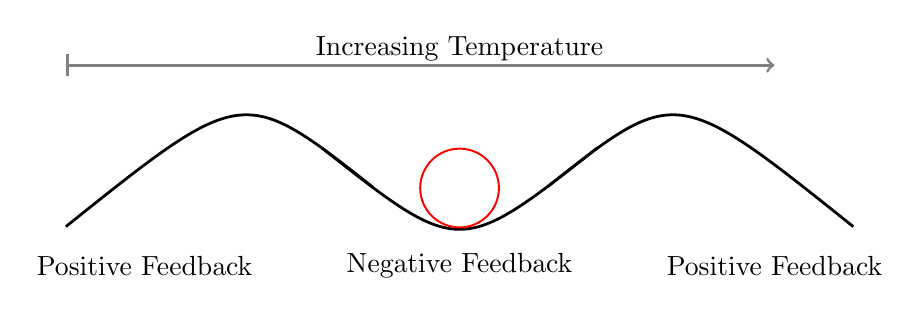
\begin{tikzpicture}[scale = 1]
        \draw[line width=1.pt] (0., -0.5) .. controls(7.75-5.5,1.3) .. (3.9, 0);
        \node at (1, -1.0) {Positive Feedback};
        %%%%%%%%% ball in bowl %%%%%%%%%%%%%%%%%
        \draw[line width=1.pt] (5+ -1.75, 0.5) .. controls(5+0,-0.88) .. (5+1.75, 0.5); 
        \node at (5, -1.0) {Negative Feedback};
        %%%%%%%%% flat plane ball %%%%%%%%%%%%%%  
        \draw[color = red, line width = 0.7pt] (5+0,-0.010) circle(0.5);
        %%%%%%%%%% ball on bowl %%%%%%%%%%%%%%%%%
        \draw[line width=1.pt] (6.11, 0) .. controls(7.75,1.3) .. (10, -0.50);
        \node at (9., -1.0) {Positive Feedback};
        \draw[|->, color=gray, line width = 1] (0, 1.55) -- (9, 1.55);
        \node at (5,1.755) {Increasing Temperature};
    \end{tikzpicture}
		
		 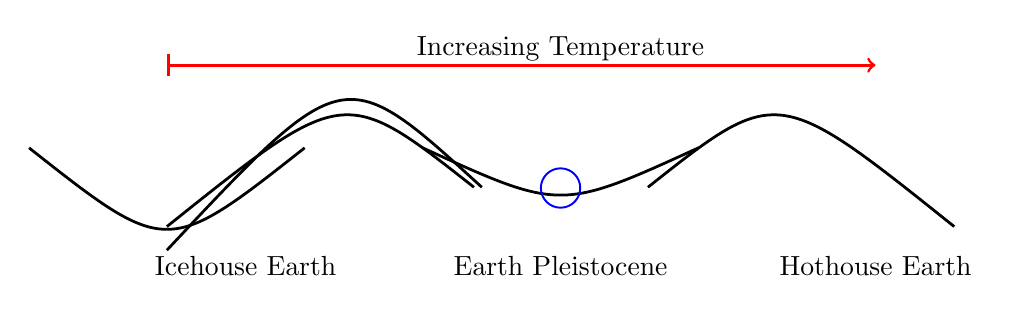
\begin{tikzpicture}[scale = 1]
				%%%%%%%%%% Icehouse bowl
				\draw[line width=1.pt] (0+ -1.75, 0.5) .. controls(0+0,-0.88) .. (0+1.75, 0.5);
				
        \draw[line width=1.pt] (0., -0.8) .. controls(7.75-5.5,1.6) .. (4.0, 0);
				\draw[line width=1.pt] (0., -0.5) .. controls(7.75-5.5,1.3) .. (3.9, 0);
        \node at (1, -1.0) {Icehouse Earth};
        %%%%%%%%% ball in bowl %%%%%%%%%%%%%%%%%
        \draw[line width=1.pt] (5+ -1.75, 0.5) .. controls(5+0,-0.30) .. (5+1.75, 0.5); 
        \node at (5, -1.0) {Earth Pleistocene};
        %%%%%%%%% flat plane ball %%%%%%%%%%%%%%  
        \draw[color = blue, line width = 0.7pt] (5+0,-0.010) circle(0.25);
        %%%%%%%%%% ball on bowl %%%%%%%%%%%%%%%%%
        \draw[line width=1.pt] (6.11, 0) .. controls(7.75,1.3) .. (10, -0.50);
        \node at (9., -1.0) {Hothouse Earth};
        
				%%%%%%%%% label temperature
				\draw[|->, color=red, line width = 1] (0, 1.55) -- (9, 1.55);
        \node at (5,1.755) {Increasing Temperature};
    \end{tikzpicture}
		
    \caption{A simplified view of the feedback processes of the earth's surface temperature. If it gets too cold, there will be a runaway albedo effect much like the ice age where more and more ice forms on the Earth. This is an example of positive feedback. As the concentration of the greenhouse gases increases, there is a point of no return and we have a runaway greenhouse effect, i.e. positive feedback. Luckily we live in a ``sweetspot'' where these forces seem to cancel each other out. }
    \label{fig:earth_stability}
    \end{figure}

    \begin{exercise}
        The planet Venus is different than Earth in several respects; First, it is 30\% closer to the sun. Next, it has thick clouds that reflect 77\% of the incident sunlight. Finally, its very thick atmosphere is much more opaque to infrared light than the earth's. Given the solar constant for Venus, which we will denote by $\mathcal{V}$ (rather than Earth's solar constant $\mathcal{S}$), takes on a value of $\mathcal{V} = \SI{2796}{\watt/(\meter^2 \kelvin^4)}$:
        \begin{enumerate}[(a)]
            \item Calculate the surface temperature of Venus if it did not reflect any incident light.
            \item Estimate the surface temperature taking Venus' albedo into account.
            \item The atmosphere of Venus absorbs roughly 70 times the amount of infrared light of that of Earth's atmosphere. We can model this with 70 successive atmospheric shells like we did in Sec.~\ref{sub:shell_atm} with \underline{each shell at a different equilibrium temperature.} The temperature of the top layer will be what you found in part (b). The next layer is warmer by a factor of $2^{1/4}$. The layer below that is warmer by a smaller factor. Keep working your way down until you see a pattern.

            Use this to estimate the surface temperature of Venus. The measured surface temperature of Venus is $\SI{740}{\kelvin}$; how does your answer compare? This is a good illustration of the runaway greenhouse effect.
        \end{enumerate}
        Note: this is a challenging problem! Don't worry if you don't get it immediately! 
        \label{ex:venus}
    \end{exercise}
    
    % subsection the_atmosphere (end)    

    % section the_atmosphere (end)

%%%%%%%%%%%%%%%%%%%%%%%%%%%%%%%%
%% CONNECT TO REST OF TEXTBOOK
%%%%%%%%%%%%%%%%%%%%%%%%%%%%%%%%

\section{Greenhouse Gases in Asia} % (fold)
\label{sec:gg_in_asia}

\subsection{Gross versus Per Capita GHG Emissions}

After seeing the potential for the greenhouse effect to raise the surface temperature, we should look at carbon dioxide emissions around the world. Specifically, we are going to focus on Asia's emissions. The Asian economy is made up of more than 4.5 billion people which is significantly more than half of the world's population. In addition to this, Asia is the largest and fastest growing economic region in the world, according to the International Monetary Fund. In addition to this, the Organization for Economic Cooperation and Development (OECD) projects that Asia will remain the fastest growing economic region in the world through 2030. All the while, the population and energy demands of the region (and world) will increase. Economic growth and greenhouse gas emissions---specifically carbon dioxide---have been linked together \citep{saidi2015impact}.

\begin{figure}[ht!]
    \centering
    \includegraphics[width = \textwidth]{emissions3.png}
    \caption{The relative emissions of East Asian and Pacific countries (excluding the high income population) compared to the world taken as a whole. Data taken from the World Bank and is current up to 2014 \citep{WBco2,WBmethane}.} 
    \label{fig:asia_emissions}
\end{figure}

As you might expect, a rapidly growing economy needs to produce a large amount of energy. Currently, a cheap and convenient form of energy is \textbf{fossil fuels}, which are natural fuels that formed millions of years ago from the remains of organisms. Some examples of fossil fuels are coal, oil, and natural gas (methane). Fossil fuels are burned in order to release energy, in the form of heat, into their surroundings allowing work to be done. However, when fossil fuels are burned, they release carbon dioxide and water into the atmosphere. Now we can make a prediction. Since Asia has and, recently, has had the fastest growing economy in the world, we would expect the emissions of the region to be rising faster compared to the rest of the world. This is exactly what we see in Figure~\ref{fig:asia_emissions}. Since the early 2000's, there has been a steady and relatively constant increase in the amount of both carbon dioxide and methane into the atmosphere. In comparison to the rest of the world, East Asia and the Pacific are releasing significantly more carbon dioxide per person and methane per year into the atmosphere. However, Asia---as a continent---has a significantly higher population than the the rest of the world.

This release of greenhouse gases will, as we saw in our toy model, lead to an increase in average surface temperature of the earth. This change will affect many aspects of the earth.  This is why people are concerned about releasing greenhouse gases into the atmosphere. When the average surface temperature of the earth warms, it causes large problems in ecosystems. This phenomena is called \textbf{climate change} and is at the forefront of international and scientific communities because of its potential consequences. Climate change and its consequences will be of central focus to the rest of this book.

\begin{figure}[hb!]
    \centering
    \includegraphics[width = 0.8\textwidth]{Vostok_Petit_data.png}
    \caption{Correlation between the temperature of the earth with the concentration of carbon dioxide over a timescale of 420,000 years. Data is taken from the Vostok ice core in  The current concentration of carbon dioxide is over 400 parts per million (ppm). Taken from Wikipedia.}
    \label{fig:ice_core}
\end{figure}

% section greenhouse_gases_in_asia (end)

%%%%%%%%%%%%%%%%%%%%%%%
%% CONCLUSION 
%%%%%%%%%%%%%%%%%%%%%%%

\section{Conclusion} % (fold)
\label{sec:conclusion}

The earth, although it may seem large to us humans, is merely a pale blue dot when compared to the solar system as a whole. Almost the entirety of Earth's energy comes from the sun. In fact, at the top of the atmosphere, we receive \SI{1370}{\watt} of power for every square meter, or one solar constant. With this, an important greenhouse effect, and little else, over the course of billions of years, life has managed to not only start but thrive. Some of the organisms that lived and died millions of years ago have converted into fossil fuels  by geologic processes. 

Today, almost the entirety of the world is dependent on burning these fossil fuels for energy, to fuel growing economies, to power our lights, and even produce the food we eat. However, extracting and burning these fossil fuels has and will continue to release potent greenhouse gases into our atmosphere--contributing to one of the most pervasive positive feedback loops of our generation: global climate change. Because fossil fuels are so integral to the world's infrastructure today, we should look at them more closely. This is the topic of our next chapter.

% section conclusion (end)


%%%%%%%%%%%%%%%%%%%%%%%%%%%%%%%%%%%%%
%% APPENDIX: SYMMETRY OF MOLECULES
%%%%%%%%%%%%%%%%%%%%%%%%%%%%%%%%%%%%%
\newpage
\section*{\label{app:symmetry}{\LARGE{Appendix A:}}\\The Symmetry of Molecules and Greenhouse Gases}

    In this appendix we are going to focus on how various molecules are able to move around. Specifically, we will look at how molecules translate, rotate, and---most importantly---vibrate. Now why do we care? How molecules are able to move plays a fundamental role in what type and how much energy they absorb. We will learn why some gases it the atmosphere are greenhouse gases and some are not.

    In order to make this appendix tractable, I'm assuming that you have some basic chemistry background already.

    \section*{Chemical Bonding} % (fold)
    \label{sec:bonding}
            
    Molecules, quite simply, are atoms that are bonded together via \textbf{chemical bonds}. Chemical bonds are the links between atoms \citep{atkins2014physical} There are a few different types of common, chemical bonds that we see around us in Nature:
    \begin{enumerate*}[(1)]
        \item covalent bonding,
        \item ionic bonding, and
        \item metallic bonding.
    \end{enumerate*}
    In this appendix, we are mainly going to focus molecules that are held together through covalent bonds; another name for these molecules are covalent compounds. \textbf{Covalent bonds} are bonds in molecules where different atoms will share pairs of electrons in order to reduce their energies. For example, water, methane, and carbon dioxide have each of their respective atoms bonded together like this.

    When molecules are formed, their shape is determined by minimizing the repulsion from the negatively charged electrons surrounding the various atoms in the molecule \citep{atkins2014physical} This comes about from various lone pairs of electrons that originate with covalently-bonded molecules. Lone pairs of electrons are assumed to be more repulsive than bonded atoms. Because of this, molecules take the shape as to maximize the separation of these lone pairs.\footnote{For an understanding of how these molecules take these shapes, I recommend reading any general chemistry textbook or a good online resource like \texttt{www.khanacademy.org/science/chemistry/chemical-bonds} about valence-shell electron pair repulsion (VSEPR) as well as Lewis Structures.} 

    We will look at the geometric shapes a few different molecules that will frequently appear, except for sulfur hexafluoride, and are relevant in this text: carbon dioxide (CO$_2$), water (H$_2$O), methane (CH$_4$), and sulfur hexafluoride (SF$_6$). All four of these molecules are \textbf{polyatomic molecules}, meaning that there is more than one type of atom present, e.g. hydrogen and oxygen constitute the elements of water, sulfur and fluorine are the elements found in sulfur hexafluoride, etc. 

    \begin{figure}[ht]
        \centering
        \includegraphics[width = 0.55\textwidth]{molecule_shapes.png}
        \caption{The geometric shapes used to describe symmetric, polyatomic molecules. In our examples, CO$_2$ is linear, H$_2$O is angular (or bent), CH$_4$ is octahedral, and SF$_6$ is octahedral. Figure taken from Atkins' \emph{Physical Chemistry} \citep{atkins2014physical}}
        \label{fig:shapes}
    \end{figure}

    Carbon dioxide is a linear molecule with the carbon atom in the middle of two oxygen atoms, water is a bent molecule, methane is tetragonal, and sulfur hexafluoride is octahedral. All four of these molecules' shapes can be visualized in Figure~\ref{fig:shapes}.

    Some atoms are more \textbf{electronegative} than others. That is, some atoms attract electrons more strongly than others. The net result of this leads to a partial negative charge (denoted $\delta^-$) near the atoms that are more electronegative and a partial positive charge (denoted $\delta^+$) located somewhere else on the molecule. When this occurs and there is an unequal sharing of electrons, we say that that the covalent bonds are \textbf{polar}. Now, when there are two opposite charges $Q$ separated by a distance $d$, then there is something that we call an electric \textbf{dipole moment}, $\mu$, whose magnitude is given by \( \mu = Q d. \) So when there are two different atoms bonded together, there will be a nonzero dipole moment. However, for the molecule \emph{as a whole}, there may not be any net dipole moment. For example, the double bond between carbon and oxygen in carbon dioxide is polar with the oxygen atom being more electronegative than the carbon. Thus, there is a dipole moment. However, since there is an identical dipole moment pointing in the \emph{opposite direction}, they cancel and thus, there is no overall dipole moment in carbon dioxide. In fact, of all the molecules we are going to discuss, only water has a non-zero dipole movement. Dipole moments will dictate the absorption of infrared light in Sec.~\ref{sec:sym_phys_prop} below \citep{atkins2014physical,harris1978symmetry,bishop1993group}

     % section bonding (end)

    \section*{\label{sec:sym_ops}Symmetry Operations and Elements} % (fold)

    Some objects are more symmetric than others. For example, a circle is more symmetric than a square. You are able to rotate a circle about its center by any angle and get a similar object. However, you are only able to rotate a square about its center by \SI{90}{\degree}, \SI{180}{\degree}, \SI{270}{\degree} and get back the same shape that you started with. Similarly, a sphere is more symmetric than a cube. An operation that transforms an object and leaves it looking the same is called a \textbf{symmetry operation.} The \textbf{symmetry element} about which a symmetry operation is performed which can be a line, point, or a plane. For example, a reflection is performed about a particular plane of an object. There are five symmetry operations that we will consider in this text:
    \begin{enumerate*}[(1)]
        \item identity, 
        \item reflections, 
        \item rotations, 
        \item improper rotations, and
        \item inversions.
    \end{enumerate*}
    We will treat and tackle each of these below.

        \subsection*{Identity} % (fold)
        \label{sub:identity}
        
        This is the simplest symmetry operation that every object has is the \textbf{identity} and is denoted by $E$. This operation tells you to do nothing to the object. The reason we include it is because some objects only have this symmetry and it is needed to satisfy certain mathematical requirements that we will not discuss here.

        % subsection identity (end)

        \subsection*{Rotations} % (fold)
        \label{sub:rotation}

        Another common symmetry operation that you may encounter is the \textbf{n-fold rotation} which we denoted by $C_n$; this means that we can rotate an object by $\SI{360}{\degree}/n$ and get back an equivalent object.\footnote{It's important to make the explicit distinction between \emph{equivalent} and \emph{identical}. An equivalent object looks like the same object that you started with. An identical object is the object that you started with. For example, rotating a triangle by \SI{120}{\degree} gives you an equivalent object whereas rotating it by \SI{360}{\degree} gives you the identical triangle.} It makes no difference whether you choose to rotate the object in a clockwise or counterclockwise direction, so long as you are consistent.In this text, we will choose the clockwise direction. 

        You can perform an $n$-fold rotation an arbitrary, integer number of times, say $m$ so long as $m$ is smaller than $n.$ We denote $m$ rotations about the $n$-fold rotation axis as $C^m_n$.  For example, if you rotate a square by \SI{180}{\degree} then you have just performed the $C^2_4$ operation which is also the same as a $C_2$ rotation. In other words \[ C_4 \cdot C_4 = C^2_4 = C_2\]. Furthermore, if you start with a square, rotate it by \SI{90}{\degree} and then rotate this equivalent object by another \SI{270}{\degree} you get the identical object that you started with. It's as if you hadn't rotated it at all! We call denote the operation that gives back the identity the \textbf{inverse.} More mathematically, we write \[C^3_4 \cdot C_4 = C^4_4 = E.\] In general, we can see that $C^{n-m}_n$ and $C^m_n$ are inverses of each other, i.e. $C^{n-m}_n \cdot C^m_n = C^{m}_n \cdot C^{n-m}_n = E.$ 

        Some simple examples would be a triangle has a 3-fold rotation axis, i.e. you can rotate the triangle about its center by $\SI{360}{\degree}/3 = \SI{120}{\degree}$, a square has a 4-fold rotation axis, a pentagon has a 5-fold rotation axis, etc. As we saw in our square example, some objects have multiple rotation axes. Consider a hexagon. You can rotate the hexagon by \SI{180}{\degree}, \SI{120}{\degree}, \SI{60}{\degree} corresponding to $C_2$, $C_3$, and $C_6$ rotations respectively. The highest value of $n$ (in this case 6) is called the \textbf{principal axis}. 

        \begin{exercise}
            Name the different $C_n$ in a cube. There should be three not including the identity operation. What is the principal axis and how many principal axes are there? (\emph{Hint:} Look at the corners and edges of the cube.)
        \end{exercise}

        % subsubsection rotation (end)

        \subsection*{Reflections} % (fold)
        \label{sub:reflection}

        The next symmetry operator, one that is likely familiar to you, is the \textbf{reflection} through a plane which is denoted by the Greek letter $\sigma.$ The mirror plane can either be parallel or perpendicular to the principal axis. If the mirror plane is parallel, we label the mirror plane $\sigma_v$ where the $v$ stands for ``vertical'' and if it is perpendicular we label it as $\sigma_h$ where $h$ stands for ``horizontal.''

        \begin{figure}[ht]
            \centering
            \includegraphics[width = 0.35\textwidth]{mirror_planes.png}
            \caption{An example of the two different mirror planes that correspond to the water molecule. Figure taken from Atkins' \emph{Physical Chemistry} \citep{atkins2014physical}}.
            \label{fig:mirros}
        \end{figure}

        Note that if you perform two reflections across the same plane in a row you get exactly what you started with, i.e. it's as if you performed the identity operation; more mathematically, we would describe it as such: $\sigma \cdot \sigma = \sigma^2 = E$. Therefore, we see that $\sigma$ is its own inverse.

        \begin{exercise}
            How many reflection planes does a square have? A rectangle?
        \end{exercise}
         % subsubsection reflection (end)

        \subsection*{Improper Rotations} % (fold)
        \label{sub:improp}

        This next symmetry operation is a little trickier to see and most of us don't have a good intuition for it like we might with proper rotations and reflections because it is a combination of the two. First you rotate the object by some amount and then reflect the object across a mirror plane that is perpendicular to the axis of rotation. See Figure~\ref{fig:improp_methane} for a visualization of this. We call this an \textbf{improper rotation} and denote it with the symbol $S_n$. The inverse of $S^m_n$, in general, is $S^{n-m}_n$ if $n$ is an even number and $S^{2n-m}_n$ if $n$ is an odd number. Can you see why we must make this distinction between $n$ being odd versus even?

        \begin{figure}[ht]
            \begin{center} 
            \begin{subfigure}[b]{0.35\textwidth}
                \includegraphics[width = \textwidth]{improper_methane.png}
                \caption{Methane}
                \label{fig:improp_methane}         
            \end{subfigure}
            ~
            \begin{subfigure}[b]{0.33\textwidth}
                \includegraphics[width = \textwidth]{improp_ethane.png}
                \caption{Staggered Ethane}
                \label{fig:improp_ethane}         
            \end{subfigure}
            \caption{\textbf{(a)} A visualization of one of methane's three $S_4$ symmetry operations. First you rotate the molecule by \SI{90}{\degree} ($C_4$) and reflect it across the horizontal plane ($\sigma_h$). While neither the $C_4$ or $\sigma_h$ operation is a symmetry operation of methane by itself, by combining them together we see the molecule is indistinguishable (or equivalent) from what we started with. \textbf{(b)} Similarly for ethane only with at $S_6$ rather than $S_4$. Figure taken from Atkins' \emph{Physical Chemistry} \citep{atkins2014physical}}
            \label{fig:improper}
            \end{center}
        \end{figure}
        
        % subsubsection improper_rotation (end)


        \subsection*{Inversion} % (fold)
        \label{sub:inversion}
        The final symmetry operation we will go over is \textbf{inversion} which is represented as $i$ in symbolic form.\footnote{This is not to be confused with the same $i$ you may have encountered in a mathematics course previously where $i = \sqrt{-1}$ by definition.} We imagine passing each point in an object through its \textbf{center of symmetry} and placing it on the opposite side. If a point initially has the coordinates $(x,y,z)$ then after the inversion the coordinates will become $(-x,-y,-z).$ It turns out that this operation is equivalent to an $S_2$ operation (i.e. $i = S_2$), but inversion's importance warrants the distinction. An example of an object is the staggered ethane molecule shown in Figure~\ref{fig:improp_ethane}. Note that inversion is its own inverse.

    \begin{exercise}
       Find and sketch an objects that has inversion symmetry.
    \end{exercise}
        
        % subsubsection inversion (end)
    \begin{exercise}
     The Great Pyramid of Giza is one of the world's seven ancient wonders. Name and draw seven symmetry operations it has.
     \label{ex:giza}
    \end{exercise}

    \begin{exercise}
        Name all of the symmetry operations for
        \begin{enumerate*}[(a)]
            \item carbon dioxide,
            \item water,
            \item methane, and
            \item sulfur hexafluoride.
        \end{enumerate*}
    \end{exercise}

    % subsection symmetry_operations (end)    

    \section*{Physical Properties and Symmetry} % (fold)
    \label{sec:sym_phys_prop}

    Now at this point, you may be wondering why we went over this discussion of symmetry, much less in an environmental science textbook. The answer is that symmetry plays a fundamental role in how the natural world works around us.\footnote{
        The details are not important, but if you think of various conservation laws you may have heard of in various sciences courses (e.g. conservation of energy, conservation of linear and angular momentum, conservation of charge, etc.) all arise from various symmetries of systems that we are studying. This isn't important to this text, but it does show how interesting Nature is.
        } 
    So it should be no surprise that properties (both physical and chemical) arise from the symmetries of its structure. 
    
    Molecules can essentially do three things. They can translate across space. They can rotate. And lastly, they can vibrate.

    Now let us consider a single particle floating in free space by itself. There are only three ways for it to move, either in the $x$, $y$, and $z$-directions respectively. Because there are three ways for it to move, we say that there are three \emph{degrees of freedom.} Now when there are two particles moving together in free space, there are a total of six degrees of freedom. Three of the six include simple translation. That is, the molecule can move around. There are two ways it can rotate. This is a subtle point that only holds for diatomic molecules. In Figure~\ref{fig:diatom_dof}, we see that there is no way for a diatomic molecule to rotate about its $z$-axis, leaving one degree of freedom left for vibration. 

    \begin{figure}[ht]
         \centering
         \includegraphics[width = 0.45\textwidth]{diatom_dof.png}
         \caption{The six degrees of freedom of a diatomic molecule. Notice that there are only two ways that it can rotate. The rotation about the $z$-axis does not change the location of the atoms, and thus, does not count (However, in any non-linear molecule, there will be a $R_z$ rotation). Because of this, there is a remaining degree of freedom: a vibrational one. Figure taken from Harris' \emph{Symmetry and Spectroscopy} \citep{harris1978symmetry}}.
         \label{fig:diatom_dof}
     \end{figure} 

    In principle, we can continue to just add more and more atoms to the molecules, making them bigger and bigger. With each atom, we get three more degrees of freedom. When the molecules are not linear, six of the degrees of freedom are contained within translation and rotation. The remaining degrees of freedom are turned into various vibrations of the molecule. To summarize, in a molecule with $N$ atoms, if the molecule is \emph{linear} there are $3N -5$ vibrational modes; if it is not linear, there are $3N-6$ vibrational modes.

    \begin{exercise}
        How many modes of vibration are there for 
        \begin{enumerate*}[(a)]
            \item carbon dioxide,
            \item water,
            \item methane, and
            \item sulfur hexafluoride?
        \end{enumerate*}   
        \label{ex:vib_numbers}
    \end{exercise}

    A logical next question would be, why do we care how many vibrational modes a molecule has? Quite simply, the answer is that when one of these vibrational modes is excited, the molecule \emph{absorbs} energy. Molecules can be thought of various atoms attached together with springs (the covalent bonds). When you have a mass on a spring, you can put energy into the system by displacing the mass by either compressing or stretching the spring. When you release the spring, the mass will vibrate back and forth. The same thing happens with molecules. The covalently bonded atoms act in the same way only with light exciting the bonds (springs), allowing the molecule to absorb energy and later radiate it back towards the earth contributing to the greenhouse effect.

    Now depending on the symmetry of the molecule, that is what symmetry operations each molecule has, determines how a molecule can vibrate. The different ways a molecule can vibrate are called \textbf{vibrational modes}. Here is the key concept to take away: a molecule will only absorb infrared radiation if the vibrational mode \emph{changes the overall dipole moment of the molecule.} \citep{harris1978symmetry,atkins2014physical,bishop1993group}. When a molecule absorbs IR-radiation, it is said to be \textbf{infrared active}. To further illustrate this, we will look at the case of water and carbon dioxide as seen in Figure~\ref{fig:vib_modes}. 

    \begin{figure}[hb]
     \begin{center}
        \begin{subfigure}[b]{0.6\textwidth}
            \includegraphics[width = \textwidth]{h2o_vibs.png}
            \caption{Vibrational Modes of H$_2$O. Figure taken from Harris' \emph{Symmetry and Spectroscopy} \citep{harris1978symmetry}}
            \label{fig:h2o_vibs}         
        \end{subfigure}
        \begin{subfigure}[b]{0.6\textwidth}
            \includegraphics[width = \textwidth]{co2_vibs.png}
            \caption{Vibrational Modes of CO$_2$. Figure taken from Harris' \emph{Symmetry and Spectroscopy} \citep{harris1978symmetry}}
            \label{fig:co2_vibs}         
        \end{subfigure}
        \caption{Here are the vibrational modes of water and carbon dioxide. Every single way that either of these two molecules can vibrate is some combination of the modes given above. Only some of these are infrared active \citep{harris1978symmetry} N.B., the underbrace below the rightmost CO$_2$ vibrational modes are there to suggest that these are excited by the same energy, i.e. they are degenerate.}
        \label{fig:vib_modes}
     \end{center}
    \end{figure}    

    The dipole moment of water that is not vibrating, has a net dipole moment where the negative charge is centered near the oxygen atom and the positive charge is centered directly between each of the hydrogens.\footnote{
        Imagine drawing an arrow of length $d$ from the positive to the negative charge as a visualization of $\mu.$
        }. 
    If you go through each of the three vibrational modes of water given in Figure~\ref{fig:h2o_vibs}, then you will see that either the distance or direction of its this arrow, its dipole moment, will change. Consequently, each of the three ways that water can vibrate will absorb IR-radiation. However, if we look at carbon dioxide in Figure~\ref{fig:co2_vibs}, we see the left-most vibrational mode has zero net change in carbon dioxide's dipole moment as there is still an equal but opposite dipole moment pointing from the carbon atom to each oxygen; consequently, that vibrational mode is \textbf{infrared inactive.}

  
    Now we are finally understanding how important a molecule's symmetry actually is in determining its potency as a greenhouse gas. In the case of methane\footnote{Check out \texttt{http://www.chemtube3d.com/vibrationsCH4.htm} to visualize the vibrational modes of methane.} and sulfur hexafluoride,\footnote{Check out \texttt{http://www.chemtube3d.com/vibrationsSF6.htm} to visualize the vibrational modes of SF$_6$.} there are a relatively high number of atoms (5 and 7 respectively) leading to $3N - 6$ vibrational modes. If a molecule is highly symmetric, then essentially any vibration will change it's nonzero, net-dipole moment, leading to vibrations in the molecule that will absorb (and eventually re-emit) infrared radiation. This, coupled to with the lifetimes of these molecules in the atmosphere, make highly symmetric molecules much more potent greenhouse gases. As human-induced greenhouse gases (mostly carbon dioxide and methane) are the main contributers to climate change, it is important to understand how and why these gases have the relative potency that they do.

    \begin{exercise}
        Which of the following molecules are greenhouse gases: N$_2$, H$_2$, CF$_4$, and N$_2$O. Why?
        \label{ex:greenhouse_examples}
    \end{exercise}
    % section symmetry_and_physical_properties (end)



%%%%%%%%%%%%%%%%%%%
%% ANSWER KEY
%%%%%%%%%%%%%%%%%%%%%
\newpage
\section*{\label{app:answers}{\LARGE{Appendix B:}}\\Answers to Selected Exercises}
    \textbf{Solution~\ref{ex:kelvin}}: \begin{enumerate*}[(a)]
        \item \SI{273.15}{\kelvin}, 
        \item \SI{373.15}{\kelvin}.
    \end{enumerate*} \\
    \textbf{Solution~\ref{ex:humans}}: \begin{enumerate*}[(a)]
        \item \SI{734.51}{\watt}, 
        \item Assuming 2000 Cal/day: 32\% of food energy goes to body heat.
    \end{enumerate*}
    \\
    \textbf{Solution~\ref{ex:venus}}: \begin{enumerate*}[(a)]
        \item \SI{333.2}{\kelvin}, 
        \item \SI{230.8}{\kelvin}, and
        \item \SI{669.8}{\kelvin}.
    \end{enumerate*}   
    \\
    \textbf{Solution~\ref{ex:giza}}: $E,\, C_4,\, C_2,\, 4 \sigma_v.$ \\
    \textbf{Solution~\ref{ex:vib_numbers}}: 4, 3, 9, 15.  \\
    \textbf{Solution~\ref{ex:greenhouse_examples}}: CF$_4$, N$_2$O.
\chapter{Heat Transfers: Evaporation, Transpiration, and Precipitation}\label{ch:evapotranspiration}
\chapterauthor{Marc Los Huertos}

\section{Hydrological Cycle}

\subsection{Solar Radiation as a Driver the Hydrological Cycle}

The suns energy powers the hydrologic cycle in Earth. And the hydrology effectively creates weather. 

As describe in Chapter~\ref{ch:earth_sun}, the sun heats the planet's atmosphere. While keeping our planet well above 0 degrees C made life as we know it possible, it does alot more. 

First, the heat drives weather patterns, and for our purposes now, it drives the hyrologic cycle.  

\subsection{Heat and Evaporation}

\subsubsection{Evaporation and Evapotranspiration}

The heated atmosphere allows the air to hold more air -- thus increases the rate of evaporation. The water vapor in the atmosphere can then be redistributed by air currents.

Water is lost directly from plants as well -- but it forms a tight linkage to soils, where evapotranspiration is the loss of water via stomata in leaves that has traveled through the vascular system of plants, the roots and soil. 

\subsubsection{Potential Evaporation}

However, just because the air is warm enough and it can 'hold' more water doesn't mean it will. The difference between water that is actually evaporated and what could be evaporated is termed as potential evaporation. When biomass is related to potential ET we see a strong correlation. 


\subsection{Precipitation: Rain and Snow}

\subsubsection{Temperature}

Water the atmospheric temperature falls below a certain temperature... 
thus, the atmosphere can no longer hold water. 

\subsubsection{precipitation and Elevation}

These changes in temperature can depend on the height of the air mass. As air masses heat they also rise, as the air mass go up in temperature, the temperature declines and can'tholdwater, thus, it rains.


\subsubsection{Orographic Effects}

\subsubsection{Rain and Latitude}


\subsection{Tropical Zones}

The tropical zone, loosely defined as the region between the Tropic of Cancer and Tropic of Capricorn (latitude XX and -XX). The region has rainfall that often exceeds XX mm per year and a mean annual temp of XX and at lower elevations never any frost events. 

The vegetation is adapted to XXX 

\subsubsection{Desert Regions}

\subsection{Temperate Zones}

\subsection{Monsoons}

Much of east Asia is temperate --- but as one moves south the climate become increasingly tropical. The temperate zone is defined by ... however, we are now confronted with the monsoon -- which was coined for the weather of east asia, we will explore the monsoon weather as we begin to unpack weather patterns with more detail (Chapter~\ref{ch:climate}). 


\section{Static versus Dynamic Views of the Climate System}

\subsection{Paleoclimates versus Climate Change}

As shown in Chapter \ref{ch:earth_sun}, the Earth has experienced dramatic shifts in climate over a record of 100 thousand years. Thus, the climate of the Earth, the average of weather is non-stationary or static. The Earth's climate is dynamic and sensitive to various factors (forcings) that lead to warming or cooling.

Since the Holocene (~18,000 years ago), the Earth has been warming. The warming has driven changes in weather patterns, as the patterns of how heat is distributed can be disrupted. The shift to a warming climate became with metaling glaciers and caused by XXX???, but even this warming has been interupted, by various events, such as the ``Little Ice Age''. What cause this event is subject to much debate, but was likely caused by...

\subsection{Climate in the Anthropocene}
 
Meanwhile, the Earth's climate has been on an accerated increase in temperature, over and above the warming post the Holocene. Although the exact amount that is due to natureal cycle and anthropogenic causes might be considered controversial by some, we have a pretty good idea that the average energy entering the Earth is higher because of greenhouse gases. This increases the amount of energy in our earth's weather systems. We will dicuss the implications of these changes in Chapter \ref{ch:climate}. 

\section{Conclusion}

The upward and downward transfer of heat and rain define the basic weather patterns on planet Earth, but as we'll see in Chapter~\ref{ch:climate} the lateral transfer of heat and moisture with winds provide yet another process that help use understand how weater and climate works. Once we understand these additional factors, then we can better appreciate the complexity of climate and its dynamic nature.  Stay tuned.
\chapter{Converting Solar Energy in Organic Carbon: Phytomass}
\chapterauthor{Allison Joseph and Maddie Nelson\footnote{Statement of Contributions: }}

\section{Introduction}

\subsection{Tropical Forests: Stored Solar Energy}

The tropical rain forests of Southeast Asia are a part of the earth's oldest existing tropical ecosystems They are believed to be some of the most biologically diverse ecosystems, their biodiversity and richness unparalleled by that of the Brazilian Amazon and African tropical rain forests. They also represent a significant portion of the Earth's biomass --- created by the sun's energy via photosynthesis and relatively high levels of precipitation.

However, when one searches academic databases on the topic of SE Asia ecosystems, the researcher is confronted with a plethora of studies focused on dire predictions on the deforestation in SE Asia. So why are so many scientists concerned about the tropical forests in SE Asia? Are they that unique?  What makes them special?

\subsection{Biodiversity Hotspots}

It's popular to cite locations that have high levels of biodiversity, but these indicies are often focused on a specific taxa, e.g. amphibians, orchids, beetles, etc. For example, South East Asia has the highest global diversity for a number of taxa when analyzed at a family level (\url{http://www.iucnredlist.org/}). 

However, the level of taxonomic uncertainty associated with many taxa may be significantly higher than other parts of the world, with only a small proportion of many large taxa described (i.e., 50\% of bats; Francis et al. 2010), and this lack of knowledge makes regional prioritization challenging. This taxonomic uncertainty and rapid rate of species description extends across taxa with over 2216 described between 1997 and 2014 (i.e., see WWF‐Greater Mekong 2008, 2009, 2010, 2011, 2012, 2013, 2014), and consequently, many species in the region may be driven to extinction while still undescribed.

Before we look at the conservation issues, let's look at the ecological drivers that promote biodiversity as we first look at how photosynthesis and plant diversity can drive other types of diversity. 

\section{Primary Production}

\subsection{Plant Biomass and Productivity}

\newglossaryentry{biomass}{
	name=Biomass, 
	description={living and dead things produced by living organisms.}
	}
	
\Gls{biomass} can be defined as the total amount of above ground organic matter in trees, shrubs, and herbs including twigs, leaves, branches and bark. Measures of biomass are expressed as mass per unit area \citep{brown1991biomass}. Without context, measures of ecosystem biomass is not all the engaging. However, when we compare ecosystems, the relative amounts generate more interest. For example, the amount standing biomass found in the tropics is quite exceptional (Table~\ref{tab:biomass}), where tropical rainforests have over twice the standing biomass as the next highest ecosystems. 

\begin{table}[htb]
\centering
		\begin{tabular}{llll}\hline
Ecosystem 						& Biomass	& NPP		& R$_t$ \\ \hline\hline

Tropical Rainforest		& 45,000	& 2,000	& 22.5 years \\
Boreal Forest					& 20,000	& 800		& 25 years \\
Temperate Grasslands	& 1,500		& 500		& 3.0 years \\
Lakes									& 20			& 500		& 15 days\\
Open Ocean						& 3				& 125		& 9 days \\ \hline	
		\end{tabular}
	\caption{biomass}
	\label{tab:biomass}
\end{table}
	
Biomass is also the product of productivity -- such as annual primary production (mass per unit area per year). Annual primary productivity  on depends on a host of environmental factors which determine the physiological processes in plant growth. Without water limitations, the productivity in tropical rainforests are exceptionally productive. 

\subsection{Gross and Net Primary Productivity}

The importance of forests in the carbon cycle depends on the extent of the forest, the amount of carbon stored per unit area (as plant body or as organic material in the soil), and the rate at which carbon is ``fixed'' by the plants during photosynthesis. The rate of fixation of carbon by photosynthesis is the \textbf{gross primary productivity (GPP)}. Some fraction of this fixed energy is used by primary producers for cellular respiration and maintenance of existing tissues. The remaining fixed energy is referred to as \textbf{net primary production (NPP)}. NPP is the rate at which all the plants in an ecosystem produce net useful chemical energy. It is equal to the difference between the GPP and the rate at which they use some of that energy during respiration\citep{corlett2014ecology}. 

\begin{figure}[ht]
    \centering
        \includegraphics[width = 0.55\textwidth]{npp.png}
    \end{figure}

The ratio of NPP to GPP - the carbon-use efficiency - is widely assumed to be around .5, but there is evidence to suggest it varies over a wider range \citep{delucia2007forest}. Some, but not all components of the total NPP can be measured directly. Field studies usually measure the two largest components: the above-ground biomass increment (the increase in the dry mass of above-ground plant parts over a measurement interval of one to several years), and the fine litter fall (the dry mass of above-ground plant parts that is produced and shed during the measurement interval for the biomass increment) \citep{ruimy1996turc}. 
  
\subsection{Photosynthesis}

\newglossaryentry{photosynthesis}{
	name=Photosynthesis, 
	description={is cool.}
}

Plant biomass originates by conversion of solar energy whee the photosynthetic processes converts atmospheric CO2 into organic carbon (Figure~\ref{fig:photosynthesis}).
 
   \begin{figure}[ht]
    \centering
        \includegraphics[width = 0.55\textwidth]{photosynthesisequ.png}
				\caption{Photosynthesis}
				\label{fig:photosynthesis}
    \end{figure}
		
Although this process is the basis for much of what we rely, it's important to appreciate the mechanisms of this process because it will help us understand why different ecosystems might have different levels of productivity. 

Through the process of \gls{photosynthesis}, chlorophyll present in plants absorbs light energy the from the sun, this is called the light reaction and is, in general, composed of two steps (Figure \ref{fig:light_rxn}). The majority of light captured by the plants are in the wavelengths between the visible and near infrared portions of the electromagnetic spectrum 400 to 1100 nm \citep{stenberg2010visible}. The light-absorbing pigments that are effective in photosynthesis have absorption bands in this range.

\begin{figure}[htb]
	\centering
		\includegraphics{graphics/light_rxn.jpg}
	\caption{Light reaction}
	\label{fig:light_rxn}
\end{figure}

Chemical energy is created by the light reaction in the form of an electrical gradient, which is used create ATP --- the energy currency inside of cells. The ATP is then used to create 5-carbon sugars that can be used to fix CO2 from the air. The Krebs Cycle is a common mechanism for plants to fix carbon dioxide and then recycle the 5-carbon sugar fix more CO2 (Figure~\ref{fig:krebs-cycle_med}). 

\begin{figure}[htb]
	\centering
		\includegraphics{graphics/krebs-cycle_med.jpeg}
	\caption{Krebs cycle}
	\label{fig:krebs-cycle_med}
\end{figure}


The final result is the creation of glucose, an energy-rich organic compound used as an energy source or building block for more complex compounds (Figure~\ref{fig:Major-catabolic-and-anabolic-pathways-in-mammalian}). 
  
\begin{figure}
	\centering
\includegraphics[width=1.00\textwidth]{graphics/Major-catabolic-and-anabolic-pathways-in-mammalian.png}
	\caption{cat and anabolic}
	\label{fig:Major-catabolic-and-anabolic-pathways-in-mammalian}
\end{figure}

    
The biomass produce can also be thought of potential energy --- where energy is released by respiration (Chapters~\ref{ch:soils} and~\ref{ch:peatlands}, or converted to fossil fuels (Chapter~\ref{ch:fossilfuels}) or burned in fires (Chapter~\ref{ch:peatlands}). 

This process allows for the continuation of plant growth, serving as the the ultimate source of biomass production in ecosystems. Thus, the quantity of biomass in a forest is a result of the difference between production (through photosynthesis) and consumption (by respiration and harvesting processes).

  \begin{figure}[ht]
    \centering
        \includegraphics[width = 0.55\textwidth]{graphics/photosynthesis.jpg}
        \caption{The process of photosynthesis.}
    \end{figure}
    

\begin{problem}
  Plants need water, carbon dioxide, and light for photosynthesis. According to the diagram, how does the plant absorb water for photosynthesis? 
\begin{enumerate}[(a)]
    \item Through the leaves
    \item Through the chlorophyll
    \item Through the roots
    \item Through the sun
\end{enumerate}  


\end{problem}

Answer: C

\begin{problem}
According to the diagram, where does the plant get the energy that powers photosynthesis?
\begin{enumerate}[(a)]
\item From chlorophyll
\item From sunlight
\item From carbon dioxide
\item From water
\end{enumerate}  

Answer: B
\end{problem}

\subsection{Biomass and the Carbon Cycle}

Studies of the flow of energy and matter have acquired new urgency over the last decade in the response to the need to understand the potential role of natural ecosystems in the mitigation of anthropogenic carbon emissions.

   Carbon, in its many forms, is exchanged among the atmosphere, oceans, and land. This is called the carbon cycle \textbf{(see Fig. 1.3)}. A critical part of the carbon cycle takes place in forests. Forests exchange large amounts of CO2 and other gases with the atmosphere and store carbon in in their leaves, wood, and roots. The carbon stored in the plants and soils is called \textbf{sequestered carbon}. The carbon that is returned to the atmosphere when it has been used by trees or other organisms as energy for life is called \textbf{respired carbon}. 
  
    \begin{figure}[ht]
    \centering
        \includegraphics[width = 0.55\textwidth]{graphics/carboncycle.png}
        \caption{The Carbon Cycle. Plants take carbon dioxide (CO2) from the atmosphere and turn it into biomass (wood, leaves, fruits etc.) through photosynthesis. By extracting fossil fuels (oil, gas and coal) from deep in the Earth, we are overloading the atmosphere with carbon, and changing our climate in irreversible ways. In addition, changes in land use, such as deforestation for agriculture, represent a smaller fraction, roughly 15\%, of CO2 emissions each year. Source The Wilderness Society}
    \end{figure}


\subsubsection{Primary Production}


  
  
  
  The tropical forests of Southeast Asia account for about one-fifth of the world's forest, and cover around 26\% of the land area in the region \textbf{(See Fig. 1.4)} \citep{brown2003state}.These ecosystems are characterized by vertical layering of vegetation and the formation of distinct habitats for animals within each layer. On the forest floor is a sparse layer of plants and decaying plant matter. Above that is an understory of short, shrubby foliage. A layer of trees rises above this understory and is topped by a closed upper canopy the uppermost overhead layer of branches and leaves.
  
Although tropical rainforests form less than half of the total forest on earth, their leaf systems comprise approximately 70\% of the world's total leaf surface area \citep{gower1999direct}. In addition, the temperature and and sunlight profiles of tropical rainforests are stable in comparison to other terrestrial biomes. Their location on the equator provides more solar radiation and therefore more opportunity for primary productivity. Overall, a consistent amount of daily sunlight and lack of temperature seasonality allows for year-round growth.   It is not surprising, then, that tropical rainforests account for between 30\% and 50\% of net primary productivity in terrestrial systems, although they cover only 6\% of the total land area of the earth \citep{houghton2005aboveground}. This means that they store more carbon per unit area than any other type of ecosystem. Thus, tropical forests are critical ecosystems in mitigating the carbon cycle of the planet. 
  
 
 \begin{figure}[ht]
    \centering
        \includegraphics[width = 0.55\textwidth]{graphics/forestcover.png}
        \caption{Forest/non-forest classification of the study area, displayed with 0.25-degree resolution. A database was generated of estimates of geographically referenced carbon densities of forest vegetation in tropical Southeast Asia for 1980. A geographic information system (GIS) was used to incorporate spatial databases of climatic, edaphic, and geomorphological indices and vegetation to estimate potential (i.e., in the absence of human intervention and natural disturbance) carbon densities of forests. The resulting map was then modified to estimate actual 1980 carbon density as a function of population density and climatic zone. \citep{brown1991biomass}.}
    \end{figure}



\section{Plant Biodiversity and their Role in Biodiversity}

\subsection{What causes biological diversity?}

There is no definitive answer to what causes biological diversity. in spite of dozens of thoughtful scientists to evaluate these issues, we are left with educated guesses, waiting for others to text a range of models, evaluate emperical data, etc. ...

\subsubsection{Temperature}
	Aside from the sun, the abundance of biomass in forests is influenced by many factors, such as soil humidity, soil and air temperature, solar radiation, precipitation and soil nutrient availability. One of the most important factors influencing biomass is temperature. Optimum temperatures for plant growth are dynamic since they change with the species and varieties, duration of exposure, age of the plant, and stage of development\citep{marshall1988environmental}. However, the important plant metabolic processes, such as photosynthesis, are influenced by the temperature. Temperature also influences the absorption of water and nutrients, which ultimately affects the plant growth. In addition, soil nutrient availability is another factor influencing plant growth. Both nutrient deficiency and toxicity negatively affect total biomass and fruit production \citep{chatzistathis2013soil}. Thus, by controlling the optimum levels of nutrient availability in soil, the production of biomass can be maximized. In the cases of limited nutrient availability in soils, fertilization is a common practice adopted by the farmers in order to ameliorate the low nutrient status. 

\subsubsection{Geology}
	The high species richness and endemism in Southeast Asia is linked to its complex geological history \citep{sodhi2004southeast}. The tropical forests of Southeast Asia are the oldest, consistent rain forests on Earth, dating back to the Pleistocene Epoch 70 million years ago \cite{hutchison1989geological}. During this formation period, the rest of the world went through cooling and warming periods, but the climate of the Southeast Asian region remained more or less the same. This was due mainly because of its location on the equator and being surrounded by water. Because the climate on the equator does not change much and the surrounding oceans provide plenty of moisture in the form of rain, the region was able to have consistent forests over very long periods of time. 

  As sea levels rose and fell through warming and icing cycles, small pockets of forests survived as reservoirs of wildlife from which various species could re-establish themselves \textbf{(See Fig. 1.2)}. When the glaciers melted and sea levels rose many of these reservoirs were cut off from each other. This forced species to developed their own distinctive evolutionary paths in response to local environments, leading to an amazing diversity of species of every kind.
  
   \begin{figure}[ht]
    \centering
        \includegraphics[width = 0.55\textwidth]{graphics/geology.jpg}
        \caption{Postulated distribution of land and sea in Southeast Asia in the Cenozoic. A. 30 mya. B. 20 mya. C. 10 mya. D. 5 mya. Figures from \cite{hall2002cenozoic}.}
    \end{figure} 

\subsection{Structure and Function of Ecosystems: Biodiversity}

 As these ecosystems have been disrupted, Southeast Asia's loss of forest biomass has had significant impacts on levels of biodiversity. \textbf{Biodiversity} is defined as the variety of life and its processes, including genes, species, communities, ecosystems and the ecological and evolutionary processes that keep them functioning \citep{noss1994saving}. 
 
 Biodiversity is dependent on the presence of biomass in an ecosystem, studies finding diversity to be positively correlated with the increased presence of biomass \citep{cardinale2007impacts}. Southeast Asian forest biomass provides habitat for a diverse array of organisms, including thousands of vertebrate, invertebrate, lichen and fungi species. These species interact with each other and the environment, providing a diverse array of important ecosystem functions and services. Examples of ecosystem functions that depend on the presence of biomass include soil organic matter supply, contributions to soil development and productivity, and nitrogen fixation \citep{humphrey1999relationships}.
 
 The balance among the many factors sustaining these environments has been increasingly threatened over the last century, as Southeast Asia has lost large percentages of biomass and species diversity.  Over the last 15 years alone, 14.5\% of the region's forest cover has been destroyed \citep{gullison2007tropical}.  In countries like the Philippines, where deforestation has leveled 93\% of the country's original forest cover, there is little left to be saved \citep{sodhi2004southeast}. Vietnam has suffered the highest rate of forest destruction in recent decades, losing 43 percent of their forest cover, according to an analysis of satellite imagery. The scope of biomass loss and deforestation was highlighted by the conservation group the World Wildlife Fund (WWF), which noted that from 1973, near the end of the Vietnam War, to 2009, the greater Mekong region lost nearly one-third of its remaining forest cover \citep{sunderland2012evidence}. The impacts of this devastation are substantial in one of the world's biodiversity hotspots, as there has been large decreases in biomass quantities and available habitats for species. Most remaining forests exist in relatively small and isolated fragments, allowing only the most adaptable species to survive.
 


 \begin{figure}[ht]
    \centering
        \includegraphics[width = 0.55\textwidth]{graphics/extinction.jpg}
        \caption{This figure illustrates the population extinctions in Singapore and Southeast Asia. Green and blue bars represent recorded and inferred extinctions in Singapore, respectively. Yellow and red bars represent minimum and maximum projected extinctions in Southeast Asia, respectively. \citep{sodhi2004southeast}}
    \end{figure}


 

\section{Deforestation}

\subsection{Unprecedented Rates of Land Conversions}

Southeast Asia is losing its forest coverage faster than any other tropical region in the world. It is predicted that Southeast Asia could lose three quarters of its original forests by 2100 and up to 42\% of its biodiversity \citep{sodhi2004southeast}. Scientists fear that the current rate of deforestation could cause these rain forests to completely vanish in a hundred years. 

Before we understand the causes and implications of these losses, it's important to note that the loss of forests and grassland has been a long-term trend that has been part of the development processes in every corner of the world. For example, the loss of the great prairies in the eighteenth and nineteenth Centuries amounts to a XX loss of the stored carbon on Earth at the time and XX of the CO2 emissions. Thus, it's important to reflect that the changes experienced by regions of the world have similar drivers and consequences and requires a sophisticated ethical evaluation of these drivers, lest we cast stones before understanding the globalized processes that drive these changes. 

\subsection{Causes and Consequences of Deforestation}

Although not all deforestation is intentional, some resulting from natural factors like wildfires, human impacts and involvement have caused a disproportionate amount of destruction. Most notoriously, the region's forests are endangered and threatened by conversion to agriculture, logging (both legal and illegal), and encroaching oil palm plantations. The human impacts on the rain forests in Southeast Asia have driven many endemic tropical plant and animal species to the brink of endangerment and even extinction. 
 
Understanding the varied impacts of deforestation are complex, however, this chapter will focus on the formation and destruction of forest biomass in Southeast Asia, a critical component of tropical ecosystems. The presence of forest biomass is essential to the existence of plants, animals and atmospheric processes. Forest biomass greatly influences the global carbon cycle, bio-geochemical processes, and biodiversity.  In addition, forest biomass serves as a habitat for millions of species. However, destruction of forest biomass ultimately alters the interactions between the land surface and the atmosphere, disrupting healthy ecosystem structure and functioning. 

\subsubsection{Access Roads and Globalized Wood Products}

Unfortunately, the tropical forests of Southeast Asia are constantly changing as a result of harvesting and conversion to other land cover. Since the East Asian Miracle in 1990, the FAO (Food and Agriculture Organization) estimates that 38.7 million hectares of primary and other naturally regenerated forest have been lost in the Asia Pacific region an area greater than the size of Japan (Figure \ref{fig:deforestation} \citep{faoun163agriculture}. The rapid socio-economic development in Southeast Asia particularly infrastructure, agriculture and industrial development has affected the level of timber production and other forest ecosystem services. In addition, this loss of forests has a profound effect on the global carbon cycle. Tropical deforestation accounts for at least a quarter of all anthropogenic carbon emissions, with both the highest rates of deforestation worldwide and, as a result of high forest biomass, the highest carbon emissions per hectare cleared \citep{corlett2014ecology}.

    \begin{figure}[ht]
    \centering
        \includegraphics[width = 0.55\textwidth]{graphics/carbonstock.png}
        \caption{Deforestation and degradation rates in Southeast Asian countries, 2000-2010. Includes carbon in living above- and below ground biomass. Source: \citep{faoun163agriculture}.}
				\label{fig:deforestation}
    \end{figure}

\subsubsection {Agriculture}

Deforestation occurs in many ways. Most of the clearing is done for agricultural purposes - both grazing cattle and planting crops. Often poor farmers chop down a small area (typically a few acres) and burn the tree trunks, a process known as Slash and Burn agriculture. Intensive, or modern, agriculture occurs on a much larger scale, sometimes deforesting several square miles at a time.

\subsubsection{Palm Oil Plantations}

Found in everything from shampoo to donuts, palm oil is now the most common vegetable oil in the world and also one of the world's leading deforestation drivers. The large majority of palm oil production occurs in just two countries, Malaysia and Indonesia, where huge swaths of tropical forests have been cleared to make way for oil palm plantations. This transition is responsible for releasing large quantities of carbon into the atmosphere while shrinking habitats for a multitude of endangered species. Between 2000 and 2010 palm cultivation in Malaysia was responsible for 2 to 9 percent of worldwide emissions from tropical land use \citep{carlson2013refined}. 

\subsubsection{Logging} 

Commercial logging is another common form of deforestation. Logging can occur selectively - where only the economically valuable species are cut  -or by clear-cutting, where all the trees are cut. Logging activities are responsible for at least 50\% decline in the Southeast Asia's forest carbon density \citep{hawthorne2011impact}. Logging affects the ecological processes in timber concessions by removing biomass, manipulating forest structural characteristics, changing light regimes, and altering microclimatic conditions at both the ground and canopy levels. Logging also introduces people into the forest, increases access via logging roads, and generally increases disturbance. 

\subsection{Sociopolitical Forces}

The motivators for deforestation are very complex. A competitive global economy drives the need for money in economically challenged tropical countries. At the national level, governments encourage modern agriculture or sell logging concessions to raise money for projects, to pay international debt, or to develop industry. The logging companies seek to harvest the forest and make profit from the sales of pulp and valuable hardwoods such as mahogany. Similarly, palm oil plantations or large cattle pastures often replace rainforest to sell their commodities in the world market. 

\subsubsection{Monocultures of the Mind}
South Asian scholar, Vandana Shiva, emphasizes that the regions transition towards industrialism and economic productivity has materialized as traditional local knowledge values of the forest have been systematically undermined \citep{shiva1993monocultures}. This knowledge and power nexus has largely arose in the context of globalization and its associated set of values based on commercial capitalism \textcolor{red}{[This section is not useful, you are going to have to justify these arguments with much more depth and precision. For example, all capitalism is commercial, i.e. relies on selling things. Let's chat about what you want to accomplish here]} \citealp{king1993politik}.

\section{Conservation Efforts}

\subsection{Biodiversity Hotspots and Conservation Priorities}  

In our opinion, it's a rather weak argument as a case to protect biodiversity because 1) it sets up a perverse competition between cites for conservation dollars thus ranking some ecosystems over others using somewhat meaningiless measures and 2) privileges certain taxa over other environmental values or ecosystem processes.

\subsection{Traditional Ecological Knowledge}

\subsubsection{Swidden Agriculture}

\textcolor{red}{[ARE WE GOING TO TALK ABOUT TRADITIONAL ECOLOGICAL KNOWLEDGE -- IF SO, GET TO IT....]}

This transition is best illustrated in the dominant knowledge and practice of forestry and agriculture. Most local knowledge systems have been based on the life-support capacities of tropical forests, not on their commercial timber value. Traditional food systems based on the forest, either directly, or indirectly have been seen as non-existent in the field of vision of a reductionist forestry and a reductionist agriculture even though they have been and still are the sustenance base for many communities of the world. For example, the rainforests of Southeast Asia supply all the food needs of the Kavan, Kenyah, the Punan Bah, the Penan who gather food from the forest and practice swidden agriculture (1999). The plant supplies are gathered mostly from the surrounding forest, and some 223 basic plant types are regularly consumed. The most important food items are mushrooms (kulat), ferns (paku) and the hearts of various plants (ubot) which include bamboo shoots, wild palms, and wild bananas \citep{hong1987natives}.

Deforestation has been happening for centuries on a smaller scale. However, since the introduction of modern forestry and agriculture, plant biomass has been split into separate non-overlapping domains on the basis of separate commodity markets to which they supply raw materials and resources. In local knowledge systems, the plant world is not artificially separated between a forest supplying commercial wood and agricultural land supplying food commodities. The forest and the field are in ecological continuum, and activities in the forest contribute to the food needs of the local community, while agriculture itself is modelled on the ecology of the tropical forest. In this model, some forest dwellers gather food directly from the forest, while many communities practise agriculture outside the forest, but depend on the fertility of the forest for the fertility of agricultural land. In contrast, the global capitalist industrial complex splits forestry from agriculture and reduces forestry to timber and wood supply \citep{de1989economic}. The creation of fragmented categories thus blinkers out the entire spaces in which local knowledge exists - knowledge which is far closer to the life of the forest and more representative of its integrity and diversity.





\begin{problem}
What is the effect of biomass on ecosystem biodiversity?
\begin{enumerate}[(a)]
\item Biomass has no impact on biodiversity.
\item Increased biomass results in high rates of biodiversity.
\item Increased biomass results in lower rates of biodiversity 
\end{enumerate}
\end{problem}

\begin{problem}
The fragmentation of forests:
\begin{enumerate} [(a)]
\item Increases the number of species, reducing competition for food resources
\item Creates isolated habitats, upon which species biodiversity increases
\item Decreases biodiversity, allowing only the most adaptable species to survive
\item Is a preferred method of forest conservation
\end{enumerate}
\end{problem}

\begin{problem}
True or False: Mono-culture forests produce higher rates of above ground biomass than mixed species forests.

False. Mixed species forests produce higher rates of above ground biomass and biodiversity.
\end{problem}


\subsubsection{Case Study: The Javan Rhinos}

  Large mammals, such as the Javan rhino, are especially vulnerable to forest degradation because they require large areas of forest to survive. The Javan Rhino is a herbivore, whose source of food depends on lowland rainforest biomass. The Javan rhino is primarily a browser,  its diet consisting of shoots, twigs, young foliage and fallen fruit. 

 The Javan Rhino was declared extinct in Vietnam in 2010, due to the compounding effects of poaching and deforestation \citep{brook2014lessons}. In addition to inadequate response to heavy poaching of rhinos, forest habitats well-suited to rhinos were disproportionately impacted by deforestation and fragmentation for agricultural plots.  Conservation efforts, which commenced in earnest during the late 1980s, proved too late for the Javan Rhino.  It is now the hope that lessons learned from the Vietnamese population of rhinos may be used to protect the remaining population in Indonesia.
  
   \begin{figure}[ht]
    \centering
        \includegraphics[width = 0.55\textwidth]{graphics/javan.jpg}
        \caption{This figure illustrates the population extinctions in Singapore and Southeast Asia. Green and blue bars represent recorded and inferred extinctions in Singapore, respectively. Yellow and red bars represent minimum and maximum projected extinctions in Southeast Asia, respectively. \citep{sodhi2004southeast}}
    \end{figure}

  
  The remaining Javan rhinos live within the Udung Kulon National Park, located on a small Indonesian Island. Although protected, the park and its surrounding forests are under pressure from human activities. In addition, the rhinos find themselves threatened by the invasive Arenga palm, which is having a devastating impact on the plants that the rhinos rely on for food. The palm has spread to cover more than half of the area inhabited by rhinos, shading out the under-story and reducing the amount of plants available to the rhinos. This decreased availability of food reduces the carrying capacity of the park and slows the breeding rate of the rhinos.

  Recently, there have been talks of re-locating a small number of the remaining Javan Rhino population and forming a second, independent population.  Conservationists are concerned about the risk of natural disasters on the Indonesian island. Increased tectonic and volcanic activity threaten the rhinos, as well as the compounding threat of tsunamis due to these natural disasters \citep{setiawan2018preventing}.  However, without the appropriate amount of forest space and biomass, the 62 remaining rhinos will not survive in a new location. 

\begin{problem}	
	Discuss:
Is saving the Javan Rhino worth the time, money and effort of conservationists? Why or why not? 
\end{problem}


\subsection{Conservation and Forest Management}

The complexity of addressing the threats facing Southeast Asian tropical forests have made the region a top conservation priority. However, environmental apathy, corruption, poor natural resource governance, poverty, lack of data, and lack of conservation funding remain formidable challenges for conservationists in Southeast Asia \citep{sodhi2004southeast}.

Scientists of the WWF and other experts believe that it is essential to begin preserving the greater Mekong region's forest. The Vietnamese government has been heralded for its reforestation efforts, yet, these programs largely consist of monoculture tree plantations that harbor limited biodiversity and decreased biomass. Results of long-term experiments in Southeast Asia have examined the effect of tree species biodiversity on aboveground biomass quantities. Forest mixtures and corresponding monocultures were compared on the same site to control for outside environmental variables such as climate or weather. The study found that the productivity of mixed-species forests was 15\% greater than the average of their corresponding monocultures, and not statistically lower than the productivity of the best corresponding monoculture \citep{sunderland2012evidence}. Thus, the greater biodiversity of mixed species forests produced statistically significant higher rates of above ground biomass.

The presence and continued supply of biomass represents a key concern in managed forest systems  Overall, conservation responses will need to be strategic, addressing the need for long-term development and employing temporary measures to secure species and ecosystems under imminent threat. Future conservation policies will act as living documents in response to the regions they represent. Multiple actions will be needed, ranging from initiatives at international, regional and national policy level to many thousands of projects, negotiations and decisions at the level of sites and landscapes. 

However, the decisions by policy-makers regarding the management and use of forest and trees will require more accurate and precise information on the state and patterns and rates of change of the resource. To attain these needs, reliable estimates on the state and change of forest biomass for all countries over the long term must be made \citep{brown1991biomass}. 

\section{Conclusion}

The tropical forest biomass of Southeast Asia plays an intricate and vital role in the functioning of healthy ecosystems and atmospheric balances. However, tropical deforestation has greatly lowered quantities of forest biomass, resulting in decreased biodiversity, a disruption of ecosystem service and the endangerment of endemic species. In addition, through its essential participation in the global terrestrial carbon cycle, forest biomass has been recognized as an essential climate variable.

Forest biomass also affects global and regional climate and environmental health.  From 2002 to 2012, the degradation of forest was responsible for a 10\% increase in greenhouse gas emissions \citep{gullison2007tropical}. It is estimated that forest protection and reforestation efforts, if successful, could be powerful enough to offset greenhouse gas emissions for up to 40 years as other energy sources are developed and integrated \citep{lasco2002forest}. With booming economies, the countries of the Southeast Asia region must now balance legitimate needs for development while safeguarding ecosystem services that are under growing threat. 

Thus, in the coming decades, the preservation and management of forest biomass should remain a top priority for conservationists, government officials, and local individuals. Many scientists are currently researching the best methods of sustainable forest management, with the hope of developing practical recommendations for a modern Southeast Asia. 
%%%%%%%%%%%%%%%%%%%%%%%%%%%%%%%%%%%%%%%%%%%%
%%% COPY AND PASTE EVERYTHING ABOVE THIS %%%
%%%%%%%%%%%%%%%%%%%%%%%%%%%%%%%%%%%%%%%%%%%%
\chapter[Soils]{Soils: Atmosphere, Lithosphere and Biosphere Linkages}\label{ch:soils}
\chapterauthor{Wilfrido Batista and Israel Teru\footnote{Statement of Contributions: Wilfrido Bautista wrote the introduction to soils, carbon pollution, and agriculture (above ground carbon sequestration.}}

\section{Soils as a Living Resource}

\subsection{Soil Ecosystem Services}

\subsubsection{Soils --- Food and Water}

Soil is a resource that is non renewable and essential to life on Earth. Soil helps sustain many of the natural processes that happen on the Earth from water quality, land use, and vegetation security. 

When looking at the human production benefits for soil it literally grows the food we eat, adds fiber to paper and clothing, foundation for the roads and buildings humans make. Without soil the world as we know it would literally crumble to pieces and all chaos would ensue from the perspective of an natural scientist. Witnessing soils' natural attributes of mitigating pollutants and excess water, groundwater recharge, cycling of nutrients, and habitat for microorganism and biota. The vitality of soil is ever prevalent in the everyday lives we walk through.


\subsubsection{Carbon Sinks and Sources}

The carbon fixed by autotrophic organisms, dominated by plants biomass, drives carbon sequestration on the planet. Although XX\% of this carbon is stored in plant biomass, soils sequester a very large proportion of the carbon fixed. Thus, soils provide a conduit that stores carbon and even promotes long-term burial of carbon --- reducing global co2 concentrations --- and helping the planet maintain it's relatively warm, but not excessively hot energy balance. 


\subsubsection{Biogeochemistry of Soils}

As the main reservoirs of nutrients, soils also have an impact on the phosphorus and nitrogen cycle, which we will attempt to infuse here to capture the relationship between erosion and biogeochemical cycles. Usually these two cycles are associated with aquatic impacts, but it is crucial to open up the discourse to terrestrial environment \citep{van2007impact}. When mineralization of soil carbon occurs, so does an increase in dissolved nitrogen and phosphorous due to soil mobilization \citep{jacinthe2002carbon}. Burial of carbon can lead to the stabilization of nitrogen as seen in the consistent Carbon-Nitrogen ratios in topsoils across a given ecosystem. Nitrogen cycling can also affect carbon cycling with biomass production \citep{van2006element}. If nitrogen is a limiting factor for biomass, then nitrogen can also be viewed as a limiting factor for carbon.





\subsection{Soil Development: 4 Processes}

Four basic processes determine soil development: 

\begin{description}
	\item[Additions] is the concept of different elements and material adding to the already existing soil in the region. The materials are added to the soil through decomposing vegetation and organism or new mineral materials.  Natural elements that fall onto soil we see are water and dust added minerals. Organic particles we see is added by organic matter adding nutrients. Human influences of addition that we see in soil is fertilizer. 

\item[Losses] through the evaporation of water. When precipitation occurs we see soil particles wash away in the storm. The organic matter in the soil can erod breaking down into carbon dioxide.  Harvetation from the soil is other factor that occurs many times leading to poor soil conditions if excessive. We see physical/chemical of soil shifts leading to lost of many natural material within. 

\item[Translocations] move soil material whether organic or mineral between soil profiles. Organism that can burrow down into the soil can move materials through the soil to their benefit. We can see translocation through change in coloration differences, texture, and structure.

\item[Transformation] we see in the soil when chemical or biological process of the soil occur. We see transformation with leaf decomposition into humus. In the soil we can also see hard rock through weathering process turns into soft clay. Reduced Iron (Fe+2) in soil can react to oxygen that causes rusting.

\end{description}

\section{Vertical Patterns as Product of Pedogenesis}

\subsection{Biotic and Abiotic Factors}

Soils are the product of biologic activity -- but their development depends on a range of influential factors. 


Soils act as key players in global interfaces which are both horizontal and vertical. 

They serve as the intersection of many scientific subjects -- take hydrology for instance. Hydrology relates water to land through vertical and horizontal interactions. It is important to study hydrology because we can learn and predict about relevant environmental conditions like time and scale of flooding, distribution of moisture in the soil which relates to the distribution of plants, chemical and sedimentary transmission from the built environment to rivers, and agricultural productivity \citep{chappell2010soil}. 

In 2001, Elsenbeer fostered the notion that subsurface water pathways in the tropics start with vertical flow in Ferralsol soil and transition to lateral flow in Acrisol soil \ref{fig:ferrasol_acrisol} \citep{elsenbeer2001hydrologic}. The study has been shown to have some inconsistencies, partly a result of the better definitions that exist for soil types today. It has been found that the proportion and type of clay in the soil can lend these types of soils a wide range of vertical and lateral properties. For example, Bukit Timah in Singapore is dominated by Acrisols with kaolinite, a type of clay, and has less than 10\% lateral flow \citep{chappell2005contrasting}. Hence, generalizations like Eisenbeer's should be questioned. One can now see how picking up on such nuances is crucial to scientists.


\begin{figure}
\includegraphics[width=\textwidth]{ferrasolacrisol}
\caption{Elsenbeer's Hypothesis on the Water Pathways in Ferrasols and Acrisols}
\label{fig:ferrasol_acrisol}
\end{figure}

Taking us back to the geologic timeline, quaternary soils are known to be generally unconsolidated, also holding many hydrological properties such as fluvial (river) deposition, marine inundation, slope wash and more \citep{chappell2007runoff}. Many of the sediments in Southeast Asia are loose, attributing soil permeability to regions like the Mekong Lowland of Cambodia and Central Plain of Thailand \citep{chiem1993geo}. This means that rainfall does not simply reach river by a lateral pathway over land, instead it can often times percolate before it reaches rivers. Aquifers, large areas of underground water characterized by porosity and ease of percolation, are found in these regions \citep{struckmeier2004groundwater}. \newline

These factors include abiotic characteristics: climate, topography, parent material, and time. In many cases, the trajectory of how these characteristics influence the development of soil is via water. Water promotes weathering of minerals, and chemical and clay translocations. 

\subsection{Phytomass Drives Pedogensis}

\subsubsection{SE Asia's Tropical Forests and Soils}

Southeast Asia lies right on the equator. The equator is home to much of Asia's tropical forests thanks to its relatively intense moisture and warmth. Anyone who visits these tropical forests will notice the cramped and dense canopy level, known for being evergreen and semi-deciduous (losing leaves for a relatively short amount of time, if at all) \citep{lieth2012tropical}. At low latitudes and with heat, the growing season in tropical forests is long and the rates of decomposition and nutrient recycling are speedy. While across all ecosystems, on average, 69\% of the carbon is stored in the soil and 31\% in living biomass, these accelerated processes stimulate an allocation of is about equal in parts in the tropics \citep{dixon1994carbon}. In this respect, deforestation in the tropics is noticeably more harmful than elsewhere.


 
\subsubsection{Abiotic Factors: Role of Water}

Water also promotes the biotic factors, i.e. organisms that live in or interact with soils. With more water, we tend to see more above ground biomass. Depending on the water content of the soils, organic carbon stored in the soil can vary to a high degree.  Thus, soils provide an important mechanism to store carbon in the biosphere.


But water does much more. Chemicals and clays are transported downward or upward in the soils.
 
%storing carbon - inorganic and organic - and supporting plants which remove carbon from the atmosphere. 

%Our aim, then, is to also study the the carbon pollution and sequestration of Southeast Asia. The carbon influx we know is off balance and the implications of this are not fully understood. In this chapter, we will first give the reader the tools to understand basic soil processes and what kind of elements affect soil development in a global context. 

%We will then introduce the region's soil composition from the lens of geologists and biologists and summarize some of the most recent research concerns in the region. We will then contextualize these issues in the discourse on carbon by describing both the carbon storage capabilities of the region as well as carbon pollution in the region. In transferring knowledge and skills to the reader, this chapter cannot cover all of the information about soils and carbon, but instead it will be rooted in case studies and research that have been conducted in the region. Readers will thus learn about Southeast Asia and how to analyze like scientists. 

\subsubsection{Weathering Processes that Shape Soil}

When looking at soil formation we need to take in account the different occurrences that can affect forever changing soils. The change of soil formation are largely determined by the weathering of rock. Rock can go through three different types of weathering. \textcolor{red}{[HELP, I only see three categories of weathering, what am I missing? Perhaps Biological weathering?]}

Physical weathering is the when an adequate amount of stressed is applied to rock to break it. The processes that help in this process of physically breaking rock are erosion, freeze- thaw cycles, bioturbation, the presence of cracks or gaps in soils. 

Chemical weathering deals with the changes in the chemical nature of rocks. This occurs with mineral structure, reactivity, surface area, and particle size. The occurrences normally happen when there is instability of primary minerals at the Earth's surface, which is driven by instability of minerals. There must be exposure to the environment for the weathering process to happen. When looking at primary minerals and secondary minerals the presence of secondary minerals that are based off primary minerals show there will be a significant amount of clay. The presence of clay shows evidence for weathering because it is proof there was a secondary elements. Chemical weather increases in warmer, humid climates, with water and oxygen. We also see biological weathering with the microbial and plant root metabolism acid \citep{brady2007colloidal}. 

Chemical weathering processing can happen in four ways. Oxidation is one of the chemical processes that can happen in soil that involves high oxygen supply leading to an elemental lose of electrons. Reduction is the gaining of electrons and happens in environments where oxygen is decreasing. Hydration is the presence of water molecules in the mineral structure. Hydrolysis is hydrogen ions (water) presence in breaking down silicate structures (rock.)

\subsection{Soil Horizons versus Sediments}

As a result of the vertical structure of biological activity, e.g. above ground deposition of detritus from plants or root uptake or turnover, soils develop important vertical structure that can be identified visually. The soil layers are defined as distinct layers called horizons (See Box). %that vary depending on the topography of the terrain.

(Insert Picure and Minipage :-))

The top uppermost layer is the O horizon composed of organic matter. This top horizon can vary in abundance due to factors like erosion.  We see a great distinction in O horizon in forested habitats. Subclassification of the O horizon are seen broken into three categories called hemic (Oe), fibric (Oi), and Sapric (Oa). The hemic (Oe) is known for having decaying matter with an identifiable origin of decomposition. The Fabric matter is organic matter that much unidentifiable origin of more decomposed matter. The last subcategory is the Sapric (Oa) is completely decomposed matter with unidentifiable origins. 

The next layer the A horizon is composed of a mainly minerals forming at/below soil surfaces. We can see either the presence of organic matter in this horizon as well. And if the use of tillage (cropping preparation) has been done to the soil we can see accumulated organic matter. The A horizon and O horizon can both play part each other when if heavy cultivation occurs on the soil leading to O horizon organic material to be found in the A horizon. 

The E horizon, known as the eluvial horizon due to the its loss of clay, iron(Fe) or aluminum Al is most common mineral horizon in forest soils. The loss of these dark minerals is due a leaching of nutrient via root zone due to water movement through the soil horizons. This leads to lighter mineral color like quartz, silica, or other minerals being the most abundant in E horizon. The E horizon is seen as a lighter horizon compared to the other layers present due to this reason.

The B horizon is most commonly found below the O, A horizons and either below or above the E horizon. The B horizon receives the deposited dissolved material of clay, iron and aluminium oxide, organic matter of decay plant and animal matter, carbonates, gypsum, and leached silicates from other layers. The presence of the Fe and Al oxide give the B horizon its reddish dark color than other horizons. 

The C horizon is home to little soil influenced by weathering process. This leads to presence of more parent material which attribute to the the chemical and physical properties of soil. There is a clear transition in this horizon from soil to bedrock

The last horizon is the R horizon which consist of complete bedrock. In terms of depth into the soil where you can find R horizon it strictly depends geographic location, environmental conditions, and landscape position it can go as deep as 100 feet or a few centimeters from soil surface. Bedrock is a strong reinforced rock that has fallen to the soil properties of the terrain. The deeper the bedrock the more we see a characteristic of biochemical weathering. While newly weathered bedrock is known as saprolite/saprock 

\section{Identifying Soils}

\subsection{Soil Definition}

The definition of soil by the Natural Resource Conservation Service (NRCS) touches upon its physical definition, natural body comprised of soils (minerals and organic matter), liquid, and gases that occurs on the land surface, occupies space and is characterized by one or both of the following: horizons, or layers, that are distinguishable from the initial material as a result of additions, losses, transfers, and transformation of energy and matter or the ability to support rooted plants in a natural environment \citep{baillie2001soil}. Other definition for soils is in environmental genetics terms is, the unconsolidated mineral or organic matter on the surface of the Earth that has been subject to and shows effects of genetic and environmental factors of: climate (including water and temperature effects), and macro- and micro organism, conditioned by relief, acting on parent material over a period of time. A product-soil differs from the material from which is derived in many physical, chemical, biological, and morphological properties and characteristics. 
 
\subsection {Soil Classification Schemes}

\subsection{Geology and Soil Types}

The soils of Southeast Asia, particularly of islands in the region, are known to be generally much younger than those in Africa and the Americas \citep{juo2003tropical}. Much of the land rose from the oceans during the recent Cenozoic Era, which only spans the past 65 million years since the extinction of non-avian dinosaurs \citep{hall2002cenozoic}. 

The Quaternary period, the current period in the Era, brought a regime of monsoonal weather and limestones \citep{verstappen1997effect}, which humans have been exploiting for its initial crop productivity against acidic soils and its accessibility in low elevation \citep{asio2006morphology}. It is important to note that less pedological research (research on soils) has been conducted in Southeast Asia compared with geologically older regions, making the information presented here that much more relevant. 

In terms of soil types, Southeast Asia is an anomaly. While the Ferrasol group is the most common in the Amazon and Congo Basin, Southeast Asia is dominated by the Acrisols group \citep{kyuma1966major} -- the group covers 51\% of Southeast Asia. 

Acrisols can be found in a wide range of elevations, and they are generally confined to areas without a marked dry season. They formed on acidic to basic parent material, and in general they are relatively poor in nutrients and are susceptible to erosion. Ferrasols are also found in a wide range of elevations. They are fossil formations interacting with today's climate ranging from semi-hot equatorial to monsoon hot tropical. 

A lot of information about soils, particularly in developing nations, was consolidated through a two-decade global survey conducted by the Food and Agricultural Organization of the United Nations (FAO), UNESCO, and the International Society of Soil Science \citep{dudal2005soils}. Hence, most of the information presented here is extracted from the FAO-UNESCO Soil Map of the World Volume IX on Southeast Asia. Tables 1 and 2 present data about some of the subcategories of Acrisols and Ferrasols. These subcategories are chosen with a focus on mainland southeast Asia in mind as can be seen in Figure \ref{fig:mainlandsoils}.

Exercise 1: Find the document from the FAO-UNESCO Soil Map of the World Volume IX on Southeast Asia and add a soil subcategory to the tables below.

\begin{table}
  \caption{The data captures the characteristics of Acrisol subcategories, including properties relevant for agriculture. Information consolidated from the FAO-UNESCO Soil Map of the World Volume IX.}
\begin{center}
  \begin{tabular}{ | p{3.5cm} | p{3.5cm} | p{3.5cm} | p{3.5cm} |}
    \hline
    \multicolumn{4}{|c|}{Acrisols} \\
    \hline
    Categories & Ferric & Gleyic & Humic \\ \hline
    Tropical Forest Type & lowland evergreen rain forest & dry deciduous forest & montane rain forest | generally on non-volcanic mountain slopes\\ \hline
    Acidity & Alkaline & Alkaline &  Alkaline \\ \hline
    Natural fertility level & Low & Low & Medium \\ \hline
    Organic Matter Content & Low & Low & High \\ \hline
    Water Drainage & Low & Low & High \\ \hline
    Other Limiting Factors & iron concretions & &\\ \hline
    Agricultural Interference & requires heavy applications of phosphate, potassium and nitrogen fertilizers & requires irrigation syste for continuous water input & soil management to reduce erosion\\ \hline
    Suitable Crops & Rubber & rice & tea, upland rice, groundnuts, maize \\ \hline
    Other Comments & & dries quickly & slopes make erosion a hazard if deforested/exposed\\ 
    \hline
    \end{tabular}
		\end{center}
\end{table}
 
\begin{table}
\begin{center}   
    \begin{tabular}{ | p{5cm} | p{3cm} | p{3cm} | p{3cm} |}
    \hline
    \multicolumn{4}{|c|}{Ferrasols} \\
    \hline
    Categories & Humic & Rhodic & Xantic \\ \hline
    Tropical Forest Type & natural montane evergreen rain forest - developed from volcanic deposits & evergreen rain forest - developed on ancient basalt (type of volcanic rock) & poor evergreen rain forest\\ \hline
    Acidity & Neutral & Basic-Neutral & Neutral-Acidic \\ \hline
    Natural fertility level & Low & Low & Low \\ \hline
    Organic Matter Content & Med-High & Med & Low-Med \\ \hline
    Water Drainage & High & High & High \\ \hline
    Other Limiting Factors & often found with a layer of ironstone concretions within rooting zone & & hard layer of iron concretions\\ \hline
    Agricultural Interference & typically not used for agriculture & little phosphate and nitrogen fertilizer & typically not used for agriculture\\ \hline
    Suitable Crops & none & rubber, coffee, fruit trees, tobacco, maize & \\ \hline
    Other Comments & used for timber if anything & crumb top layer makes it resistant to erosion & should be reserved as natural forest\\ 
    \hline
    \end{tabular}
    \caption{Table 2. The data captures the characteristics of Ferrasol subcategories, including properties relevant for agriculture. Information consolidated from the FAO-UNESCO Soil Map of the World Volume IX.}
\end{center}
\end{table}

\begin{figure}
\includegraphics[width=0.90\textwidth]{mainlandsoils}
\caption{Soil Types in GMS Countries}
\label{fig:mainlandsoils}
\end{figure}

\subsubsection{USDA versus FAO versus other Classification Schemes}

Soil classification systems used by the United States of Agriculture (USDA) is the  Soil Taxonomy system \citep{soil2003keys}. The system is morphologically focused that uses quantitative and soil genesis to make soil groups \citep{buol1999oxisols}. The classification system is hierarchical with six levels that is 1) Order, 2) Suborder, 3) Great Group, 4) Subgroup, 5) Family, and 6) Series. There are 12 soil orders in the soil systems and each have differing characteristics (Box X:XX).

\fbox{
\begin{minipage}[c]{.9\textwidth}
\subsection{Box XX: USDA Soil Classification}
Entisols are known for being the youngest formed soils in soil order. They normally include weak profile of soil layer development meaning horizon difference  aren't as a differentiable. Entisols can be found in use in agricultural spaces (plow layer), steep slopes with severe erosion, and  floodplains.  

Inceptisols soil orders are characterized for being young and having little to no soil profile development at all. We find them mostly alongside rivers and streams due to this.  

Both Entisols and Inceptisols have the potential at a later time to develop intricate soil horizons. The thing playing as a major influence in these soils is parental material unlike other soils likely influenced by climate and vegetation. 

Gelisols are considered young soil orders in terms of geologic time and are found in colder climates. The condition they are found in are permaforst and cryoturbation in Canada and Alaska \citep{soil2003keys}. 

Mollisols are prairie soil mainly found in midwestern United States where they dominate landscapes. They are known to be characterized for their high organic content, dark colors, steep A horizons. The category to be met for the A horizon is that it must be 8 inches deep and must be 50\% saturated. Alfisols can be found in midwestern America as well and are normally in deciduous forest habitats. Alfisols are found in humid landscapes globally and have have E horizons.  The base saturation for these soils must be at least 35\%. 

Spodosols originate from parent material that is acidic in nature and areas of loamy/sandy content. We normally see spodols in forest vegetation like coniferous forest due to pine needles high acidity when decomposing. \citep{brady2007colloidal} We normally see the presence of a bright red horizon below a white E horizon.
\end{minipage}
}%

While these classification of soils is effective. We must be mindful that the data was created by the United States Department of Agriculture (USDA) in the 1970s. The implications of it in a global context may not cohesively translate and the way locals in native Southeast Asian countries classify things could greatly vary. A part of understanding soil is understanding the way locals interpret the data and be able to communicate across these boundaries for a better and new outlook.





\section{Human Impacts on Soils}

\subsection{Contextualizing Soils in Southeast Asia}

As mentioned, soil is fundamental to the survival of humans: from plant growth, to water purification, to decomposers in the nutrient cycles, and even to bacteria that have been used for developing antibiotics that treat human disease \citep{asio2006morphology}. Soil degradation caused by physical and chemical occurrences (like wind or loss of nutrients), are now widespread, putting tropical fauna and flora as well as humans who depend on agricultural productivity at risk. The National Action Plan of the Philippines, for instance, has identified soil degradation as a major threat to soil productivity and water retention (The Updated Philippine National Action Plan to Combat Desertification,Land Degradation and Drought, 2010). Soil degradation was coined in 1888 to describe natural soil changes, but according to the Global Assessment of of Soil Degradation has since come to define human-induced disruption because of the aforementioned urgent crises (UNEP, 1992). Let us dive into the scientific history of soils in Southeast Asia so that we can better illustrate the context with which are dealing. [as part of thesis: As we walk through this history, we will demonstrate the impact of water, as molded by natural and anthropogenic processes, on the soil.]

\subsection{A Resource in Peril}

Tropical soils in Southeast Asia are some of the fastest deteriorating soils in the world. The deterioration is the result of anthropogenic disturbances, like the burning of vegetation, and its impact is ultimately determined by the existing development patterns-the pedogenesis- of the soil. Thus, as we determine ways to mitigate soil degradation, we must learn about both human-caused assaults and the given environmental backdrop of Southeast Asia. [Proposed thesis: In assessing these two factors, we learn that hydrology, the movement of water in relation to land, is arguably the most important force in shaping soils in Southeast Asia. The region is enveloped by both the Indian and Pacific Oceans, impacted by monsoonal seasons, and contains roaring rivers like the Mekong.] 

Ever since the 1970s, the tropics overtook the temperate zones as the fastest cleared forests in the world, and since the 1990s have constituted almost all net forest clearance \citep{houghton1996land}. This is inextricably tied to carbon. Thanks to the aforementioned characteristics, tropical forests play a key role as a global carbon sink, meaning they can hold large stocks of carbon. In fact, they account for 37\% of the world's terrestrial carbon pool. This is especially crucial in the face of rapid industrialization and carbon pollution in Southeast Asia. In the past two decades, carbon emissions in the region have risen the fastest at a rate of approximately 5\% per year, and this has been accomplished with deforestation and consequent land use change \citep{dixon1994carbon}. In the next few sections, we will focus on building a knowledge bank on soils. We will then develop on the connections to carbon, and offer the reader new insights on Southeast Asia all along.




\subsection{Soil Erosion}

\subsubsection{Hydrology and Soil Erosion}

Although Southeast Asia is one of the zones most vulnerable to climate change, not enough research has been conducted about its impact on soil erosion in the region. With climate change, rainfall can sporadically increase and turn more aggressive, leading to greater soil erosion \citep{chappell2007runoff}. There are a host of reasons that may be hypothesized: soil erosion can intensify as the canopy changes in response to variable moisture in the air and ground, as cover on the ground changes in response to variable decomposition rates, and as soil moisture changes in response to variable evapotranspiration rates (rates of evaporation from the soil to the atmosphere), and as land use changes in response to economic demands. In short, the implication of climate chage exacerbate the impact of rainfall on soil erosion. 

The effects of rainfall can be even worse in slopy areas. There has been special concern in watersheds shared between countries in Southeast Asia because these border zones generally require much-needed collaboration and data-sharing.\citep{giang2017spatial} In the aforemention paper, Giang and colleagues assessed the interaction between rainfall and soil erosion in the Laos-Vietnam transnational Upper Ca River Watershed (UCRW). The UCRW is an important site for agricultural cultivation, and its hilly topography makes it especially sensitive to acute rainfall. Evidently, there is an economic incentive to implement conservation practices in the region. The study found that spatial and temporal factors should be considered. First it was observed that much of the hill-slope erosion is found in the upstream and middle stream areas. Understandably, it was also found that sediment transport would occur mostly in the wet season when it is warmer and wetter. Therefore, to protect residents and cultivation, special attention should be paid in the months between August and October. 

To slow soil erosion, both institutional and individual measures should be applied. At the administrative levels, it should be understood that groundcover other than farming and normal anthropogenic use is necessary. Rehabilitation of the land is possible with reforestation, afforestation (foresting land at which tree cover has been absent for longer), terrace farming (farming on sloped planes with a series of flat planes), as well as check dams. At the domestic level, and just as importantly for the less hilly areas (such as downstream of the UCRW), farmers can learn and practice crop rotation, cover cropping, and mulching.

\subsubsection{Agriculture and the Soil Erosion}

As we have seen, agricultural soils can significantly alter the landscape. This can also be recognized in its impact on biodiversity. Southeast Asia is well-known for being a biodiversity hotspot, with many endemic species that rely on an established and robust food web system \citep{tripathi2012tropical}. We will use a study from Malaysia on the soil bacterial community, organisms which are much less researched and appreciated by the general public, as our kickstarter. 

Research on microbial communities around the world has been concerned with comparing their activities in forests versus agricultural lands. We ask: How do the two environments structure the accompanying bacterial communities?  What are the specific environmental factors that may explain these observable differences?

The Malaysia-based study found that, in general, the bacterial community composition was most influenced by the acidity of the soil, followed by total carbon and Carbon/Nitrogen ratio. It seems that pH level is the best predictor of bacterial diversity across all tested land types, including primary forest, logged forest, and crop and pasture land. All bacterial taxa tested showed that diversity peaked at neutral pH. 

This explains why agricultural land hosted the most diversity. Farmers lime their land to offset the acidity, and they choose soils that have greater pH due to their greater crop productivity. This means that bacteria, which have intracellular neutral pH, are better suited for the agricultural soils. This is still somewhat surprising because it conflicts with the notion that some taxa are specialized to root zones of particular plants, meaning we would assume that greater plant diversity would accomodate these specializations. This may be a plausible hypothesis: bacteria that may have evolved to have traits which allow them to thrive in low or high pH are more likely to lose these specializations in the new anthropogenically-affected environment than they are to regain these adaptations to extreme conditions. We of course know that larger organisms are marginalized when forests are cleared, so instead of celebrating the more diverse bacterial community, we should interpret the ecosystem as introducing an imbalance in the food web system.

\subsection{Soil Erosion and Carbon Cycle}

As a result of agricultural erosion, large amounts of SOC and sediments are transported laterally over the Earth. There are about three steps in soil erosion: mobilization, transportation, and deposition \citep{quinton2010impact}. Eroded land exposes subsurface soil which eventually can be transported to cover what is known as topsoil. This is why research that is exclusively performed on the topsoil can bring up questionable interpretations. 

Quantifying these aforementioned fluxes is not difficult, but climate change and land use are also dynamic processes, so relying on today's calculations may not help us predict future disturbances \citep{heimann2008terrestrial}.

From a meta-analysis conducted on tropical landuse change, we find that conversion to cropland, specifically perennial crops, reduces SOC most, by about 25\% to 30\% \citep{don2011impact}. Conversion to grassland is at 12\% and secondary forest is 9\%. If cropland is afforested, on average, it can gain 29\% in SOC. Hence, agricultural cultivation can alter carbon cycling. Still, modeling such a large system can be difficult.
Interestingly, erosion over land which results in mineralization, a process by which nutrients are rendered accessible to plants, tends to be relatively unimportant because carbon inventory does not correlate well with mineralization--even though SOC transported to rivers tends to result in substantial mineralization \citep{cole2007plumbing}. 

Also, it should be noted that erosion can actually lead to both release and sequestration of carbon. When soil is disturbed, it may immediately release carbon \citep{berhe2007significance}. Sometimes, erosion means that the subsoil mixes as the new topsoil, and if it binds organic matter then we may observe intake \citep{harden1999dynamic}. The latter depends on lower rates of SOC decomposition.

\subsection{Swidden and Fallow Cultivation practices}

Swiddening, the slashing and burning of forest is an age old practice widespread in Southeast Asian countries for agricultural production. The practice is linked to many rising environmental issues in the region. The transformation that swiddening those to the land through deforestation and decomposition effects are not fully understood and need to be further researched. Going hand in hand with Swiddening is fallowing, leaving the land plowed and exposed unseeded for a few growing seasons, is steadily decreasing. The decrease in fallowing systems is leading to the system being replaced by perennial crops like rubber, fruit trees, oil palm, and timber \citep{schmidt2009assessment}. Swiddening cultivation is a effective natural resource management that requires field rotation not crop rotation relying on the fallowing to sustain the crop production. Swiddening is found in sloping upland of the systems known for being environmentally destructive contributing to erosion, negative nutrient balances and CO2 emissions \citep{de2008soil}. Swiddening cultivation has also been seen beneficial in other studies towards providing hydrology, biodiversity, and carbon storage in soil and vegetation {powell20153}. The transformation consequence of swidden cultivation on carbon emission is its contribution to 20\% of global human carbon emissions \citep{meehl2007global}.

Carbon emission begin to rise when the change of pool SOC in aboveground biomass due to land charge. The tropical lowland forest have some of the highest aboveground carbon stocks of any vegetation in the world. In Southeast Asia carbon stocks in forest have a range of 254 to 647 Mg C ha$^{-1}$. SOC serves as nutrient pool, cation exchange pool and buffer against acidity and aluminium toxicity \citep{silver2000potential}. 

\subsection{Soils and Carbon Budget}

\begin{figure}
\includegraphics[width=\textwidth]{carboncycle}
\caption{The Carbon Cycle}
\label{fig:carboncycle}
\end{figure}

Anthropogenic interference in the carbon cycle, for which you may find review in Figure \ref{fig:carboncycle}), has mostly come in the form of fossil fuel exploitation and land use change. When undisturbed land converts to agricultural land, we observe reduced carbon inputs into the soil and accelerated decomposition of soil organic carbon (SOC) \citep{van2007impact}. SOC is removed by erosion and deposited in environments that become to be known as depositional areas. Carbon flux between the soil and the atmosphere can occur through three different mechanisms: 

\begin{enumerate}
  \item Replacement of SOC from plant input atat sites experiencing erosion and decline in SOC for decomposition
  \item Deep burial of carbon and thereafter hindered decomposition
  \item Rise in the decomposition of SOC when the soil breaks down as it detaches or transports
\end{enumerate}


\subsection{Carbon Emissions from Soils}

\subsection {Mapping of Emissions through Southeast Asia}
- Work for a later date -

\subsubsection{Agriculture and Carbon Storage}

A major contributor to the shift in carbon storage influxes in Southeast Asia continues to be the need for more agricultural land to provide to the growing population and economic growth. The countries in these region will suffer the worst soil degradation because of their tropical aspect \citep{scherr1999soil}. The agricultural systems of Southeast Asia is one of the major causes of carbon fluxes imbalances. The most intensive agricultural system Southeast Asia is the lowland rice farming systems that cover 197 million hectares of land \citep{dixon2001nonalcoholic}. The rice systems are heavily irrigated systems that produce two to three times a year \citep{cassman1995extrapolating}. The lowland rice paddies depend on N fertilizer for yield. The subsidiary corps from these systems can be seen to be oilseeds, maize, root crops, soybeans, sugarcane, cotton, vegetables and fruits in all areas.



\textit{Carbon in Mangroves} 

As mentioned earlier, Southeast Asia has some of the greatest potential to serve as a carbon sink in an industrializing world. This can be seen in one of the most prominent features of the region, mangrove forests. Mangrove forests grow in tropical and sub-tropical zones, residing at the intersections of freshwater, lands, and the ocean, usually found in brackish aquatic habitats \citep{bravo2017managing}. Considering their distribution across Southeast Asia, which constitutes a third of global presence,  mangroves have ecological and economic value that should not be underestimated. For example, they are exploited for fish and shrimp farming by indigenous communities in Vietnam as well as plain timber usage. Their immense biomass alone should kickstart a discussion on their carbon sequestration capabilities.

Mangroves can play a critical role in mitigating nutrient runoff to coastal regions, which is how they are usually framed in climate change discourse. We need to add their contribution to the carbon cycle in this context. The carbon cycle is present in terrestrial and oceanic spaces and in the transition between the two. Marine sediments and organic carbon found in mangroves can speak to the carbon sequestration potential of the ecosystem.

When mangroves shed dead material, this organic material does not thoroughly decompose, but instead the carbon can be converted to fossil fuel (compression of raw humus and creation of peat). Methane emissions from mangroves is of primary concern. It has been found that salinity and sulphate inhibit methane production by engaging sulphate-reducing bacteria which compete with methanogens. It has also been discovered that temperatures between 25 degrees celsius and 30 degrees celsius are optimal for methane emissions from the subsurface to the atmosphere. 

Moving forward, land use changes must be rethought and redeveloped. Mangroves experience their harshest degradation from direct human activity. To maintain their capabilities and capacities in nutrient cycling, reforestation and sustainable management policies must go into effect. First, though, it is also important for scientists to capture data on carbon storage in mangroves more accurately.

\fbox{
\begin{minipage}[c]{.9\textwidth}
\subsection{Box X.XX  Borneo's Biomass}

Let us dive into another case study in Borneo's forests, which are shared between two Southeast Asian nations, Indonesia and Malaysia. Borneo's forests are some of the most expansive in the region and are dominated by a single tree family known as Dipterocarpaceae \citep{qie2017long}. Unlike the Amazon and Congo Basin, Borneo's carbon-dense trees have not been treated with robust research on long-term biomass balance. Thus, it has been somewhat unclear in what ways Borneo's forests act as carbon sinks and sources.

What is known is that Borneo's forests are also one of the most fragmented in the world. This introduces edge effects which hinder biomass accumulation -- some studies have shown that the negative effects are even visible 400m deep from the edges. Another severe limiting factor for these forests in their ability to serve as sinks is extreme drought events, driven by El Nino for instance. As with rainfall, droughts are becoming more intense and frequent. 

The problem we face is that there has not been sufficient formal research conducted on the stress climate change causes, and this unequivocally raises the urgency to focus on Borneo. And, at first, the possibilities seem endless: could it be that CO2 inflates the biomass of trees? Or could it be that droughts are killing trees? Does net carbon source reduce because of edge effects from fragmentation? These questions are globalized, but nuances appear in different regions. Even if all are true, how do they compete in determine the ultimaate reduction or rise in carbon sequestration?

This particular study found that extreme drought events probably do not reverse long-term biomass accumulation because they are too short. The researchers estimated that a forest, on average, must maintain about 302 hectares to remain a carbon sink, depending on its shape and how penetrative edge effects are. Edges can decrease above-ground productivity and lead to biomass mortality. It seems that if edges are managed with healthy buffer zones, forests of almost any size can sustain themselves as carbon sinks because biomass along boundaries can survive. Still, large forest reserves are needed for preserving biodiversity.

\end{minipage}
}%



\section{Summary}
[To fit with thesis: When it comes to pedogensis and carbon, Southeast Asia is a unique, releavant, and introguing region. While there are many subtopics within these fields, it seems like the interaction with water is one of the most important. As other chapters discuss sea level rise, dive deeper into mangroves, peatlands, and geologic hazards, we find that water interfaces is a recurring theme. Even before major anthropogenic expansion and interference in the soil, rainfall, rivers, and the formation of islands demonstrated the power of hydrology to transport and bury soils. As Southeast Asia capitalizes on farming, water continues to play a critical role. In this way we can observe that hydrology places man and nature in one scope, going against a prevailing grain that humans are separated from nature.]

\chapter{Peatlands}\label{ch:peatlands}
\chapterauthor {Rebecca Chung and Christine Chan\footnote{Statement of Contributions: }}

\section{Introduction}

\subsection{Peatlands}

Peatland are wetlands that are dominated by peat forming plants that originate from biological processes. Peatland make up 3\% of the earth and are mostly found in East Asia, Southeast Asia, the Caribbean and Central America, South America and southern Africa \citep{strack2008peatlands}. Peatland globally have a  significant role in storage of soil carbon. 

Forest tropical peatlands in Southeast Asia store 42,000 million metric tonnes (Mt) of soil carbon. The stability of this pool is at risk due to the recent decades of deforestation, drainage, and fire. 

Peatland are vital when it comes to biological process because of the immense amount of carbon storage you can find in the systems, carbon dioxide sink, and atmospheric methane point. Peatland contribute small portion to the emission of CH4  and N2O but the sequestration of CO2 are far greater \citep{strack2008peatlands}. The Greenhouse gases properties of peatland is a shifting role that depends on the peatlands ecology, hydrology, climate, and climate change. The CO2 emission at times can be so great that the peatland can change from a sink to a source at times. Changing vegetation can contribute to shifts in carbon sequestration due to elevated water and production.

The major actors to disturbing Peatlands natural processes  are agriculture, forestry, peat fuel extraction, and horticulture.  Indonesia 3.7 million hectares of peatland are drained and being used for agriculture. This dramatically decrease C fixation capacity and threatened greenhouse gas emissions

Peatland can serve a very powerful asset to assuring carbon sequestration and mitigate emissions in the region.

Three components have been found to contribute in the change of carbon flux between soil and atmosphere




Southeast Asia is home to most of the world's tropical peat. In these humid conditions, peat is created and conserved in the ecosystems because peat relies on a consistent source of water year-round through rainfull or humidity. Peat, the accumulation of partly decomposed vegetable matter, makes up a peatland, which is characterized as a type of wetland with peat soil and a wetland habitat. 

Palm oil, an edible vegetable oil from the fruit of an oil palm plant, grows well year-round in the climate of Southeast Asia and on the region's peatlands. An intensified global demand for palm oil can be very harmful to public health and the climate \citep{knitr2013}. International corporations rely on palm oil for the creation of different cosmetics and processed foods. These corporations therefore place enormous pressure on local farmers to transition from subsistence mixed farming to growing exclusively palm oil. To create space for palm oil plantations, local farmers in Southeast Asia use an agricultural method called slash-and-burn, in which they burn the peatlands for large-scale palm oil plantations. Because these fires are unregulated and difficult to control, air pollution in the region has intensified. Many of the inhabitants in Southeast Asia are familiar with what is called the Southeast Asia Haze. The quality of air in Southeast Asia has deteriorated severely recently. Coinciding with a fall in air and water quality in the region is an expontential growth in demand for palm oil. 

\begin{figure}
  \includegraphics[width=\linewidth]{arifpicture.jpg}
  \caption{NPR captured a picture of the farmer Arif Subandi and the burnt peatlands near his home.}
  \label{fig:arifpicture}
\end{figure}

Beyond simply deforestation, the problem of using the slash-and-burn method on peatlands specifically is that the nature of peat makes it incredibly difficult to put out the prescribed fires. As a result, the fires burn for much longer and create much more smoke than if they were prescribed on different types of forest lands. These fires can quickly grow out of control and spread into protected forests. Fires on peatlands can then create environmental and health hazards for the local communities as well as have lasting impacts on global climate because of the magnitude of the carbon emissions. In this chapter, we will investigate the anthropogenic impacts on the environment and global climate within the context of peatlands in Southeast Asia. 

NPR covered the story of a farmer on one of Indonesia's major islands who illustrates the ecological importance and fragility of peatlands. Arif Subandi who lives in Borneo lost his family's farmland to fires on peatlands that were caused by local companies trying to use the land to create palm oil plantations (figure \ref{fig:arifpicture}). In the past, a lack of legal enforcement of bans on peatland fires and deforestation in protected areas has forced out indigenous people who live and rely on peatland ecosystems to survive. The creation of palm oil plantations for global supply chains threaten the livelihoods of farmers like Arif Subandi. Arif faces physical threats from different corporations, whether motorcycle corporations or palm oil corporations, to move off the land despite having cultivated it for many generations. 

In Indonesia, specifically, the lived experiences of people who live near peatlands illustrate how damaging certain agricultural techniques can be to the livelihoods of rural people and the natural environment. Because Indonesia produces much of the world's palm oil, it can be a useful case study in understanding peatlands and anthropogenic impacts to peatlands in the twenty-first century. 

\section{What is peat?}

Peat is an organic fuel consisting of partially or completely decomposed organic matter. The organic matter is primarly different kinds of plants and is composed when this organic material has accumulated in a water-saturated environment. The plants that form peatlands tend to be more resistant to decay than ordinary plant litter and one example of a plant that commonly forms peatlands is the Sphagnum species \citep{holden2005peatland}. Sphagnum is a genus of about 380 species of mosses that are called peat mosses. Both living and dead Sphagnum mosses can hold enormous masses of water. Because these plants are more resistant to decay than plants in other ecosystems, the immersion of water combined with this slow rate of decay allows the accumulation of carbon. The ecosystem dynamics in the peatlands are complex. In warm climates, like Southeast Asia, the plant material can decompose more quickly. 

\citet{bridgham2008rapid} puts the amount of carbon in perspective by saying that the global peatland soil-carbon pool is 75 times larger than annual anthropogenic carbon dioxide emissions. With this comparison, it becomes very clear that the need to keep carbon sequestered in the peatlands is extremely important in preventing the release of excess greenhouse gas emissions that could further exacerbate global warming. A peatland's carbon balance can change within the span of a few years. The transition of a peatland from a carbon sink, an ecological reservoir that can absorb and store carbon dioxide from the atmosphere, to a carbon source, which is one that now releases more carbon than it stores.  

Some examples of peatlands across the globe include swamps, muskegs, bogs, fens and moors. In the United States, for example, the swamps and marshes in Florida are examples of peatlands. In Southeast Asia, the more common forms of peatlands are lowland tropical peatlands which are naturally vegetated with a mosaic of specialized closed canopy forests, which refers to a dense growth of trees in which the top branches and leaves form a canopy that light can penetrate very little of to reach the forest floor, linked to local hydrological and nutritional conditions \citep{chokkalingam2005fire}.

See \citet{dennis2005fire}? 

In the wet season, peatlands are flooded by nearby lakes and rivers to depths of up to 3 meters. In the dry season, peatlands can dry out and their water levels drop greatly \citep{chokkalingam2005fire}. Differences in the water supply create differences in what the peatland's soil chemistry, nutrient availability, carbon quality, and the appearance of the plant community composition  Regardless of the type of hydrology in a specific peatland, peatlands can best be categorized as soil-carbon pools. 

\section{How is peat formed?}

\begin{figure}{!ht}
\includegraphics[width=0.5\textwidth]{peatpeat.png}
  \caption{How is peat formed?}
  \label{fig:peatformation}
\end{figure}

Peat decompositions are mostly carried out by microrganisms that use soil organic compounds as energy substrates, and are found across northern North America, northern Europe, western Siberia, Indonesia, and Southeast Asia \citep{rezanezhad2016structure}.

Conditions of near permanent waterlogging, that is, the absence of oxygen in soil, favors accumulation of partially decayed organic matter. This creates long-term ecosystem carbon storage, also known as carbon sinks. In the modern day, these processes are heavily damaged by human activity, such as monoculture farms and logging, and changes in land use, especially in Southeast Asia \citep{page2016line}.

\subsection{Characteristics of peat}

Different peatlands will exhibit vertical movement, either daily or seasonal, based on the water availability at the time, as peat is highly compressible. Peatlands generally swell and shrink when there are changes in water storage, hydraulics, biogeochemistry, and thermal properties. 

Here are some quick facts about peat:
\begin{enumerate}

\item Peat's total porosity exceeds 80 percent! It is also dual-porosity in nature, which increases water flow and solute migration.

\item It is made up of 90 percent of water.

\item In its natural state, peat has a high degree of resistance towards fires, mainly due to a groundwater table within close proximity to the forest floor. However, rising temperatures and decrease in moisture content may reduce its effectiveness.

  \item Compressibility of peat is controlled by its physical properties, including porosity and decomposition. 
  
\end{enumerate}

\subsection{What is carbon storage?}

Tropical peatlands contain up to 90 gigatons of carbon. Most of the carbon that is stored in the peatlands is organic carbon from decomposed plants or plants that are still alive. A small amount of the carbon stored is in an inorganic form, such as in the form of calcium carbonate. Southeast Asia alone has a stock of approximately 69 gigatons \citep{page2016line}. Peatlands are a carbon sink. They help regulate global temperatures. Over time, peatlands -- under the right conditions, unencumbered by human activity, can also decrease the amount of carbon dioxide in the atmosphere. Another reason why peatlands are so efficient at creating long-term carbon stores is because heterotrophic respiration, which is a very common form of carbon loss, is largely reduced by anoxic conditions brought by high water levels \citep{hirano2009controls}. Peatland development is dependent on a variety of factors coming together at the right time.

\section{Peatland Soil}

Due to increasing climate change in the past decades, soil moisture and soil temperatures on peatlands are subject to vast change. Rising temperatures and lowered water tables cause current peatlands, which are originally carbon dioxide sinks, to become net sources of carbon instead.

\subsection{Soil Moisture}

Soil moisture, which is evaluated by the soil water table, is a significant factor that shapes the composition of peatlands among the soil-air interface. For instance, methane fluxes and carbon dioxide production is affected by both the water table position and the gravimentric moisture content.

Soil moisture is mainly affected by two factors: water-holding capacity and the ability to impede upon evaporation. Water holding capacity is largely affected by the humus layer, as during dry periods, it absorbs a large amount of water, causing minimal moisture to be able to reach the tree roots. This entails a high water holding capacity and a high ability to impede upon evaporation. Thus, as burning diminishes the humus layer, charred humus has a much lower water-holding capacity as well as a lower ability to impede upon evaporation as compared to unburned humus. Higher temperatures commonly found at a burning site also lead to increased evaporation \citep{kozlowski2012fire}.

On coarse soils, which have smaller surface areas, poor water-holding capacities lead to higher evaporation rates and a lack of water penetration. This in turn hinders growth. On finer soils, on the other hand, larger surface areas lead to higher evaporation rates and lack of water penetration. These come together to facilitate growth, particularly over the course of rainy summers.

\subsection{Soil Temperature}

Likewise, soil temperatures are also significant among the soil-air interface on peatlands. In June 1984, scientists from the University of Minnesota examined the rates of production of methane on Minnesota peat. In their study, they found that increased soil temperatures were associated with a rise in carbon dioxide and methane production on peatlands. This holds true except for data taken from the two deepest sampling points, where an increase in temperature did not induce an increase in methane production.(figure \ref{fig:soiltemperature}) \citep{williams1984methane}.

\begin{figure}
\includegraphics[width=0.75\textwidth]{Methanetemp.png}
  \caption{Effect of temperature on methane production from Cedar Creek peat samples, as published by Richard T. Williams and Ronald L. Crawford in 1984}
  \label{fig:soiltemperature}
\end{figure}

Soil temperature is dependent on two distinct factors --air temperature and artificial human input, such as as prescribed burning. An increase in soil temperature, which increases carbon dioxide levels in peat, has the effect of increasing the fertility of a site \citep{kozlowski2012fire}.

In terms of heat retention, dry humus layers are better at insulation than moist humus layers. The humus layers of artificially burned sites are also more efficient at solar radiation absorbtion, as they are warmer during growth periods as compared to unburned sites \citep{kozlowski2012fire}.

\section{What are the human-caused impacts on peatlands?}

Thus commercialization of peatlands in Southeast Asia has become commonplace with the rise of powerful multinational agribusinesses. Peatlands, as will be discussed in this section, are vulnerable to human-induced fires, climate change, commercialized land use, and more \citep{turetsky2015global}. 

Human impact has led to a multiplicity of current risks in and on peatlands. Firstly, peatlands have become increasingly vulnerable to human-caused burning, especially in tropical regions, as a result of plantation development, agriculture, and logging. Additionally, the rise in human activity has led to an increase in both unintentional and intentional fires, which has made tropical peat prone to excessive burning. This has, in turn, diminished carbon stock. In peatlands of comparatively low latitude, many fire-resistant areas have also become fire prone \citep{turetsky2015global}. The peatlands of low latitude are more likely to have moist microclimates and low-flammability soils. When a peatland is disturbed, however, there is more build-up of dry, flammable fuels and lower humidity because of a reduced tree canopy. 

More significantly, however, rising global temperatures and drainage systems as a result of human activity has led to increasing rates of mineralization. In particular, change in vegetation cover and the use of fertilizers has caused peat to oxidize in the upper peat profile, resulting in increased flux of dissolved organic carbon coupled with elevated levels of greenhouse gas emissions. This means that peatlands, which are originally a long term carbon sink, may actually become carbon emitters that temporarily benefit the economy at the long term detriment of the environment \citep{turetsky2015global}. Increasing greenhouse emission may lead to further rise in global temperatures, further increasing rates of mineralization, constituting a downward vicious spiral.

Unfortunately, in addition to many current risks, Peatlands around the world are also vulnerable to many future risks. Not only are health risks imminent, as a result of respiratory disease and human mortality that is associated with diminished air quality, the thawing of permafrost peatlands may also cause climate change to accelerate. Peat erosion (figure \ref{fig:peaterosion}) in upland temperature peatlands and a decrease in biodiversity may also result \citep{turetsky2015global}. 

\subsection{Climate change}

Anthropogenic climate change can be observed in the regional climate patterns of southeast Asia from the rise of global emissions of carbon dioxide. Climate change can impact seasonal precipitation patterns and there is the potential for peatlands to release stored carbon with the lowering of the water table. This would then create a positive feedback to anthropogenic increases in greenhouse gas emissions but came from drainage affects tree growth. 

As more carbon is released into the atmosphere, the greenhouse effect intensifies. In Southeast Asia, the greenhouse effect and anthropogenic climate change further impacts regional temperature averages. The relationship between the water table and climate change is complex but in peatlands, the plant species suffer from reduced precipitation, one of many impacts of climate change. According to \citet{ahmad2009global}, ''elevated carbon dioxide is expected to decrease stomatal conductance in most species, resulting in less transpiration per unit leaf area.''

In response to rising temperatures, peatlands in the boreal region which are underlain by permafrost are highly unpredictable. In an analysis of peat cores in Canada, the underlying permafrost caused the surface to collapse nearly to the level of the water table \citep{dise2009peatland}. This has profound impacts on the ability of the permafrost to naturally restore itself. 

\citet{holden2005peatland} estimated ``over the past 10,000 years the atmospheric carbon stored in peats has served to reduce global temperatures by about 1.5-2 degrees Celcius.'' 10,000 years on a planetary timescale is a miniscule amount of time. The past hundred years is an even smaller amount of time. Yet, human activity has reversed 10,000 years of carbon sequestration in a few decades. The transformation of peatlands from carbon stores to carbon sources has played a huge role in amplifying anthropogenic climate change. 

Climate change directly impacts plant productivity and the rate of decomposition of organic matter, which is a crucial part of the creation and sustenance of peatlands. Climate change impacts plant productivity in Southeast Asia, which already has warm temperatures, by causing reduced yields and biodiversity. It also impacts the ability of farmers to plan day-to-day operations because the predictability of weather has gone down. Climate change also has indirect effects on peatlands, including changes in hydrology, water balance, and vegetation composition \citep{bonn2016peatland}.

\begin{figure}
 \includegraphics[width=\linewidth]{verticalinterface.png}
  \caption{The vertical interface between peat and the atmosphere: carbon dioxide goes in both directions.}
  \label{fig:peatlandwatertable}
\end{figure}

\subsection{Mineralization}

The greenhouse gas budget of a peatland includes the direct release of carbon dioxide and methane as well as the mineralization of fluvial carbon from dissolved organic carbon and nitrous oxide. Fluvial carbon refers to carbon that is found in rivers. Fluvial carbon has an important role in peatlands in Southeast Asia because the geography of the peatlands is mostly at low altitudes and extend large distances along and between rivers. There are also non-carbon greenhouse gases in the greenhouse gas budget of a peatland that can have varying effects on rising global temperatures, such as nitrous oxide and methane. Carbon, however, is the most common greenhouse gas produced by human activities and the most relevant to peatlands in the region.   

\subsection{Fires}

A large majority of fires in the present day are caused by farmers who want to clear the land and by private corporations that want to create oil palm and pulp wood plantations. Peatlands are particularly vulnerable to fire damage when the forests are cleared and the water table is low after drainage. As a result, fires in peatlands transition from flaming combustion to smouldering combustion. The surface fire burns the vegetation and the smouldering fire burns under the ground, consuming the peat \citep{page2016line}. The smouldering fires burn for very long periods of time and can reignite, even after a short rainy period, depending on changing soil moisture and different levels of peat depth. Below the ground, the low temperature process is under conditions of reduced oxygen availability. This leads to incomplete combustion and intense emissions of direct carbon dioxide and methane as well as the release of toxic compounds like benzene and hydrogen cyanide. 

The number of large-scale fires on peatlands in Southeast Asia has increased greatly over the past couple of decades. Once these peatlands are burned and altered, there is a feedback loop of intensive commercial use, more fires, and the transformation of peatlands into remote swamps. Peatlands that have already been burned once and are either recovering or were only partially burned are then vulnerable to recurrent burning. This repeated burning turns these peatlands into open floodplains with the loss of peat and tree cover. These peatlands are vulnerable to further human activity because the long-term impacts of the fires on health and water quality are difficult to perceive for local communities \citep{chokkalingam2005fire}. The international corporations that contribute to the burning have little incentive to consider the impact on local communities in their commercial process and are not subject to strict regulations that could potentially preserve parts of the peatland or improve ecological health in the region. Because developing economies rely on the profits of billion dollar companies and are much more difficult to regulate, the governments of developing nations struggle to rein in the ecological damage caused by large corporations.

Fire is a tool on industrial plantations because it is much cheaper and quicker to prepare the land this way than by using mechanical technology. Farmers and corporations have little incentive from the state to change methods that are convenient to methods that are better for the environment. In the poor Indonesia Province of Nusa Tenggara Timur (NTT), because fire was an integral part of traditional agricultural practices and because of lack of development in the province, local people have little to zero understanding of modern burning practices and more sustainable fire management problems \citep{russell2007rural}. Problems caused by uncontrolled prescribed burns have deep roots in socioeconomic and cultural differences between developed and undeveloped areas in Southeast Asia. The complexity of these issues and addressing burning practices in a region like Nusa Tenggara Timur, therefore, will require an interdisciplinary approach bringing environmental science, forestry, and anthropology together.  

\begin{figure}
  \includegraphics[width=\linewidth]{pulpwoodplantation.jpg}
  \caption{On the left is a pulp wood plantation in Southeast Asia. On the right is what the peatland looked like before being burned and cleared for deforestation. The cultivation of pulp wood on peatlands resembles that of oil palm, especially during this process of preparing the land for monoculture agriculture.}
  \label{fig:pulpwoodplantation}
\end{figure}

\subsection{Land Conversion}

Peatlands are drained to create space for plantations. The drainage happens on land often without regard for the rights of indigenous people who live and rely on the land for survival. The drainage combined with a change in vegetation cover and an intense use of fertilizers leads to peat oxidation in the upper peat profile and increased flux of dissolved organic carbon and increased emissions other greenhouse gases like N2O \citep{larmola2013vegetation}. There are high rates of mineralization, which is the decomposition of chemical compounds in organic matter. Thus, this carbon sink which is built over hundreds of years creates intense short-term carbon emissions. 

Drainage of peatland leads to a large loss of the peat profile and the carbon because aerobic decomposition occurs \citep{page2009restoration}. Peatland drainage leads to peat oxidation and subsidence, which cause the peatland surface to drop to levels that enable the water table to reach and rise above the new surface quicker with high rainfall. This can cause major flooding and expose underlying mineral substrates. 

The global demand for palm oil, which is used in many products, has led to the draining and deforestation of peatland (Figure \ref{fig:peatlanddeforestation}). The story of Arif Subandi, who was forced off his land to make space for oil palm plantations, in the introduction is not uncommon in the region. Palm oil is colloquially referred to as ``green gold'' because Malaysia and Indonesia are the world's largest producers of the agro-industrial commodity \citep{othman2003linking}. Beyond the impacts that draining and deforestation have on peatlands, there are seperate negative impacts of monoculture oil palm plantations which include biodiversity loss, agrochemical runoffs from fertilizers and insecticides, land erosion, and toxic haze, which will be discussed in the next subsection.  

\begin{figure}
  \includegraphics[width=\linewidth]{peatlanddeforestation.jpg}
  \caption{An oil palm plantation created on deforested peatland}
  \label{fig:peatlanddeforestation}
\end{figure}

Peatlands are also subject to the construction of drainage channel and the construction of dams \citep{suyanto2004role}. The dams are constructed for a variety of reasons, such as extracting illegal timber. Another form of direct damage is mining that is done on the peatlands for horticulture and fuel because peat can be an early stage in coal formation, thus making it a significant resource for a nation. 

\subsection{Southeast Asia Haze}

\begin{figure}
  \includegraphics[width=\linewidth]{SoutheastAsianHaze.jpg}
  \caption{Southeast Asian Haze in Indonesia}
  \label{fig:southeastasiahaze}
\end{figure}

The Southeast Asia Haze has become infamous for its impacts on human health and agriculture. In many parts of Southeast Asia, the haze has become an annual phenomenon as human activity in the region, including prescribed peatland burns, becomes more prevalent (figure \ref{fig:southeastasiahaze}). The Indian Ocean Experiment (INDOEX) study done in 1999 found that the aerosols in the haze could drastically disrupt water availability and crop production because of the way the aersols interfere with the sunlight's breakdown of hydroxl radicals \citep{taylor2003abcs}. There is a tremendous loss of biodiversity because the haze can cover millions of hectacres of land for prolonged periods of time. The haze pollution has both immediate and long-term environmental impacts. Though an overwhelming number of the massive forest fires occur in Indonesia, the haze crosses national boundaries and is carried by winds to several neighboring countries, such as Malaysia and Singapore.    

The burning of peat, as compared to the burning of other kinds of land, is much more dangerous because of the particular matter and sulphur and nitrous oxides that are released when peat is burned. The Southeast Asian Haze is unique because of the impact that burning peat has on the atmosphere. 

The impact that the Southeast Asia Haze has had on human health is drastic and worsened in recent years. There are long-term respiratory effects of the haze. Air pollution indexes from the World Health Organization reached extremely unsafe levels because the biomass smoke contained soot particles, inorganic materials like silica, ammonia, and more \citep{sastry2002forest}. This air pollution can cause respiratory and cardiovascular diseases, of which the elderly and young are most vulnerable. Premature deaths from the haze are difficult to measure because it is on a much longer time-scale than immediate respiratory problems, but it is suggested that the haze in Southeast Asia will have long-term impacts on human health.

There are not only environmental and health impacts but also economic and political impacts from the Southeast Asia haze. The negative impacts the haze has on human health and agriculture cost Southeast Asian nations billions of USD in damage and should the magnitude of the Southeast Asian haze continue, future profits and ecological health could be permanently damaged. Future profits and ecological health are at risk, even if the phenomenon of the Southeast Asia haze is resolved, because the landscape could be damaged and take centuries to recover properly.

\begin{figure}
  \includegraphics[width=\linewidth]{peaterosion.jpg}
  \caption{Peat Erosion}
  \label{fig:peaterosion}
\end{figure}

\section{Case Studies}

\subsection{ENSO Events}

The El Ni\~{n}o-Southern Oscillation (ENSO) phenomenon is a cyclical warming of the eastern equatorial Pacific Ocean. It occurs every three to five years and lasts anywhere from six to eighteen months (figure \ref{fig:elnino}). ENSO, unlike La Nina, brings droughts to even the wettest parts of insular Southeast Asia, such as Borneo \citep{aiken2004runaway}.

Peatlands are particularly vulnerable to ENSO because it is so dependent on consistent moisture for freely draining soil. Droughts cause water levels in peat swamps to drop. In Borneo, peat swamp forests during severe El Nino droughts have been subject to fires that have consumed peat up to 50cm in the late twentieth century \citep{turetsky2015global}.

In El Nino drought years, the prescribed burns in peatlands can burn with greater intensity than in more climatically stable years. With dry lakes, low river levels, and dry peat soils, strong winds during El Nino can help ignite fires or spread fires that had already been started intentionally by human activity \citep{chokkalingam2005fire}.  

\begin{figure}
  \includegraphics[width=\linewidth]{elnino.png}
  \caption{A model of global El Nino climate impacts during the peak of an El Nino-Southern Oscillation event.}
  \label{fig:elnino}
\end{figure}

The ENSO phenomenon that led to drought conditions was associated with high air pressure over the region that prevented the smoke haze from dissipating. As a result, the haze spread horizontally but managed to maintain a high level of concentration. In cities, the haze led to an atmospheric inversion and trapped emissions from cars and factories within the city. The high air pressure makes it difficult for the smoke haze to dissipate in cities in Southeast Asia because there is a large mass of high-rise buildings in the cities. The exact causes of the trapped haze are still unknown but one theory is that it is similar to the heat island effect, in which changes to the landscape cause urban regions to become warmer than their rural surroundings. 

\subsection{Indonesian Peatlands Borneo}

Indonesia allows for a concrete examination of peatlands, contributing around 10 to 12 percent of all global peatland resources. In particular, Borneo contains subcoastal peatlands that began to accumulate 22,000 to 23,000 years ago, although, sadly, recent anthropogenic activities have destroyed many of such resources. An example of such would be the burning of peatlands, induced by farmers, in order to establish pulpwood and palm oil plantations, which, though significant to the Indonesian economy, release toxic gases such as aerosols, carbon dioxide, and noxious gases, making Indonesia one of the world's largest greenhouse gas emitters. As of now, extensive deforested and drained peatlands in the region mean vast areas are not only at high risk of accidental ignition, but also cannot be used as farmland \citep{ballhorn2009derivation}.

\section{Conclusion}

The preservation and restoration of peatlands in southeast Asia requires that governments place ecological health over profit from commercialization. There are many global and regional policies that could preserve these vital carbon stocks and thus play an important role in mitigation and adaptation to anthropogenic climate change. As policymakers proceed forward to improve the ecological health of peatlands in Southeast Asia, it is important to keep in mind the need to help local people maintain their livelihoods. Preservation of peatlands will also provide an opportunity for reparations for the injustice done to indigenous peoples. 

The creation of practical programs that can support Southeast Asian countries in preventing fires during El Nino years and drought periods could provide an alternative to the common story of prescribed fires that burn out of control. Peatland restoration has the potential to boost greenhouse gas storage in the soil. Re-wetting the peat manually could play an important role in restoring vegetation and protecting the peat carbon stocks that remain after human alternation. Hydrological restoration could reduce fire risk, though its impact on reducing greenhouse gas emissions is still being studied \citep{page2009restoration}. When thinking about restoration, however, \citet{holden2005peatland} reminds us that we have to ask what we are restoring the peatlands to. Because the climate and environmental conditions today are so different from those that formed peatlands thousands of years ago, ecological restoration for a peatland could look completely different from what we might imagine as "normal." Therefore, we have to continually reexamine what ecological restoration will look like and what a healthy ecosystem looks like in the Anthropocene.

The Katingan Peatland Restoration and Conservation Project is an Borneo-based NGO that is working to help solve the problem by incorporating a business model that offers local people sustainable sources of income. In the Katingan district on the island of Borneo, there is a peat swamp forest that is bigger than Singapore. It is one of the largest remaining intact peat swamp forests left in Indonesia. The project is financed by the sequestration of carbon dioxide and is managed by an Indonesian company, PT. Rimba Makmur Utama. The project is guided by the basic principle that access to the forest will remain open to forest-dependent communities that have traditionally relied on the forest.

An international NGO that is working with local communities in Southeast Asia to preserve peatlands is the Rainforest Action Network, which is California-based (figure \ref{fig:ranpalmoil}). Where Katingan Peatland Restoration and Conservation Project is focused on providing on-the-ground solutions, the Rainforest Action Network works with the large international corporations that own the largest plantations in Southeast Asia for oil palm and wood pulp. Their aim is to encourage economic, social, and environmental sustainability within the supply chains of corporations like PepsiCo and General Mills.

\begin{figure}{!ht}
  \includegraphics[width=\linewidth]{ranpalmoil.jpg}
  \caption{A protest by Rainforest Action Network activists demanding that international corporations preserve peatlands and rainforests.}
  \label{fig:ranpalmoil}
\end{figure}

Another potential solution to peatland restoration, and thus greater planetary health, is in biomimcry. Biomimicry is the design of materials, structures, and systems that are inspired by biological processes. Biomimicry is a relatively new framework of thinking but it could be used to facilitate the creation of peatlands, which usually takes thousands and thousands of years. A question to be explored is how biomimicry can be used to improve soil quality and soil temperature. In this way, we can maintain human activity sustainably and ecological health. The two are not mutually exclusive.  

Finally, though peatlands like all other natural lands are threatened by human activity, \citet{dise2009peatland} says that peatlands are complex adaptive systems that are "resilient to change at some level of pertubation but shifting to new states at higher levels of disturbance." We must not ignore the valuable signals from the anthropogenic changes in peatlands that we are seeing now but we must also remember that peatlands, like the planet, are resilient.  



\input{chapters/007_Benthos}
\chapter{Sea Level and Coastal Elevations}\label{ch:subsidence}
%\chapter{Sea Level Rise and Subsidence}\label{ch:subsidence}
\chapterauthor{Luyi Huang and Betel Solomon Tesfamariam\footnote{Statement of Contributions: }}

\section{Introduction}

\subsection{Coastal Implications to Climate Change}

Since 1988, the Intergovernmental Panel on Climate Change (IPCC), set up by the World Meteorological Organization (WMO) and the United Nations Environmental Program, has been collating scientific research on climate change to understand the causes, evaluate the consequences, promote mitigation strategies, and coordinate international agreements to limit climate changes. 

One of the consequences of climate change is sea-level rise, and recent research calls attention to the instability of the Greenland and West Antarctic ice sheets as a factor that may result in a 1 m increase in sea-levels in the 21st century \citep{nicholls2010sea}. \citet{nicholls2010sea} examine the impact of sea-level rise in a the present-day global context whereby there is no mitigation policy and the global mean near-surface temperature could possibly reach 4 \degree C by 2100.

\subsection{Geologic Records of Sea Level Changes}
  
Sea level rise is commonly known as a global climate change event which has taken place for thousand of years as a result of changes in tectonics and consequent subsidence and uplift of  land. The relative height changes between sea and coastal lands will continue for centuries. However, certain locations will experience more or less sea level change due to the combined stratigraphic activities, resulting in local residents being impacted to different extents. Coastal and island residences are considerably being put in risk of coastal erosion, salt water intrusion, flooding and potential loss of habitats. Some questions we raise in this chapter include what contributes to global as well as local sea level rise?  Yet looking a local perspective, what are the effects brought to local farmers in Southeast Asia?

\subsection{Sea level and SE Asia}
  
Countries in Southeast Asia are especially vulnerable to global climate change because of (i) their long coastlines, (ii) high concentration of human and economic activities in coastal areas, (iii) large and growing populations, and (iv) the importance of agriculture as a source of employment and income textcolor{red}{[(ADB 2009)??]}.

Southeast Asia is at risk of being negatively impacted by climate change over the next 20 years due to the region's large and growing  population, long coastlines, abundant low-lying areas, reliance on the agricultural sector, and dependence upon natural resources. In order to understand how current sea levels around the world are changing it is useful to consider the historical context of sea level rise. 

\subsection{Chapter Preview}

This chapter will begin by providing an overview of how national governments and international organizations have responded to the reality of sea level rise and the challenges it poses for people living in coastal zones. Following this, a discussion of how sea level rise has impacted and continues to impact Southeast Asia will be offered, providing an introduction to the specific impacts of sea level rise in the Vietnamese Mekong Delta. 

The role that \CO plays in causing sea level rise will also be discussed in order to present how natural occurrences can be exacerbated by anthropogenic activity. This chapter will also present how the geological formation of Southeast Asia has historically affected sea level rise, which will lead into a discussion of the impact of isostasy on sea level rise, another mechanism that is influenced by human activities.
 
The case study of the Vietnamese Mekong Delta (VMD) is presented towards the end of the chapter to illustrate how the geographical and geological characteristics of the VMD inform our understanding of why this region is vulnerable to sea level rise.
 
This will be followed by a discussion of the processes that lead to delta formation. Natural spaces and processes are however influenced by the political decisions of humans and therefore the socio-economic and political context of the VMD will be discussed. Groundwater extraction in the VMD and dam construction in the Mekong River, two anthropogenic activities that influence how sea-level rise impacts the VMD, will be discussed in depth to reveal the ways in which transnational politics, and subsidence determine the threats posed by sea level rise and how they will be mitigated.
  
Small islands in and around Africa, Southeast, and east Asia are identified as being the most vulnerable regions to rising sea level. Coastal adaptation is a systemic process but the increased exposure to sea level rise in these regions is not being countered by a high adaptive capacity. The violent conditions of the transactional interactions between the global north and the global south result in manifestations of slow violence such as a disproportionate impact of climate change in the global south, which include the most vulnerable regions which are identified by \citet{nicholls2010sea}. 


\section{Sea Level Rise in Southeast Asia}

\subsection{SE Asia Geography as a Colonial Project}

Maps have proven to be an important analytic as well as informative source for environmental and climate research. While can be interpreted as objective knowledge, they can ``dessocialize'' the territory they represent \citep{harley2009maps}. Boundaries can differ depend on a wide range of factors related to social, political and economic characteristics of the regions being studied. Especially under colonial influence, \textcolor{red}{[the connections between maps, power and knowledge are enhancing in political geography.] not sure what this means.} The practical actions undertaken with maps: warfare, boundary making, propaganda, or the preservation of law and order, are documented throughout the history of maps \citep{harley2009maps}. 

Therefore while we use the physical maps of Southeast Asia to describe coast-sea level interactions, it's important that we acknowledge process and implication of map making as a social process with political and social values. 

The geographical region of Southeast Asia is commonly described as a corner of the Asian continent consisting of regions east of the Indian and south of China. Geographically, the region is categorized into two subregions: Indochina (the mainland Southeast Asia) and Malay Archipelago (Maritime Southeast Asia) between Pacific Ocean and Indian Ocean. 

	\begin{figure}
\includegraphics[width=70mm]{map-of-southeast-asia-region.jpg}
 \caption {Map of Southeast Asia region}
\label{fig:SEAsia}
      \end{figure}

Generally nations fall under Southeast Asia include but not restrain: Cambodia, Lao, Burma, Malaysia, Thailand, Vietnam, Indonesia, Philippines, Singapore, and Burnei (Figure~\ref{fig:SEAsia}). The region is located near the intersection of geological plates, with frequent tectonic and volcanic activities. The outer boundary of Southeast Asia is an arc formed by the islands of Indonesia and the Philippines, and area of active subduction that manifests itself in frequent earthquakes, occasional tsunamis and periodic volcanic eruptions. The inner mainland part of the region was shaped by tectonic movements associated with the collision of India with the Eurasian landmass, which has raised in Himalaya mountains over millions of years \citep{hirsch2016routledge}. %\citep{hirsch2016routledge}. 

\subsection{Tectonic History of SE Asia}

The physical geography of Southeast Asia has been formed largely by the convergence of three major tectonic crustal plates: the Eurasian, Indian-Australian and Pacific plates (Figure~\ref{fig:SE_asia_geology}). Overtime, Southeast Asia has experienced an extensive amount of geologic activities such as faulting, folding, uplifting and volcanic activity. The region includes areas with the highest global rates of plate convergence and separation. The mountains of the Alpine-Himalayan belt turn southwards into Indochina and terminate in a region of continental archipelagos, island arcs and small ocean basins. To the south, west and east the region is surrounded by island arcs where lithosphere of the Indian and Pacific oceans is being subducted at high rates, accompanied by intense seismicity and spectacular volcanic activity.

\begin{figure}
\centering
\includegraphics[width=90mm]{geology_southeast_asia.jpg}
\caption{Geology of Southeast Asia.}
\label{fig:SE_asia_geology}
\end{figure}
			

Sea level rise is a natural phenomenon that has been taking place for thousands of years. \textcolor{red}{[Woodroffe (1993) considers a series of unpublished studies on coastal and lowland river plains in Southeast Asia and northern Australia that were a product of the International Geological Correlation Programme Project 274 Coastal Evolution in the Quaternary meeting in Ipoh, Malaysia, which took place in 1989.] citation not useful, need more recent studies]} 

The evolution of the continental shelves during the Quaternary, 2.6 million years from before present, in the Cenozoic era. The extensive low-gradient continental shelves are exposed as the Sunda platform and Sahul shelf during periods of low sea level (Figure~\ref{fig:sunda}). The studies show how evolution in the Quaternary was as a result sea-level change in the region as well as environmental changes, which influenced sediment supply and alluviation. 

\begin{figure}
\centering
\includegraphics[width=70mm]{Map-of-Sunda-and-Sahul.jpg}
 \caption{The Sunda platform and Sahul shelf, which were exposed during glacial periods in the Cenozoic era.}
\label{fig:sunda}
\end{figure}

\subsection{Sea Level Change}

Since the last glaciation, sea levels have generally increased particularly after the industrialization. Ocean temperature increases as well which leads to ocean expansion. Globally averaged trend toward rising sea levels makes greater complexities. Regional effects cause sea levels to increase on some parts of the planet, decrease on others, and even to remain relatively flat in a flew places, including, in recent decades, on the California coast.

Thermal expansion of seawater can be the product of regional phenomena, such as El Nino, the periodic warming of the eastern tropical Pacific. Temperatures are increasing, leading to ocean expansion.
  
Although sea levels have always fluctuated with changes in global temperature, sea level in Southeast Asia has changed rapidly over the course of  250,000 years \citep{voris2000maps}. A study estimates and indicates that  the areas of exposed land in the Indo-Australian region during periods of the Pleistocene, when sea levels were below present levels, by producing a series of maps. The sea level changes are associated with glaciation that has taken place over the past 250,000 years BP. In this 250,000 year time frame there has been a 120 m sea level change.


\subsection{Isostasy}

The volumes of oceans increased with melting glaciers and declined with increasing glaciation. The rate of glacial melting slowed dramatically around 6000 years ago. However, there are ongoing isostatic adjustments that are a result of changes in ice load (glacio-isostasy) and changes in the load of water (hydro-isostasy), two different factors. 
  
Isostasy is a naturally occurring process that restores equilibrium between the Earth's crust and the mantle it floats on (Figure~\ref{fig:isostasy}). The mantle is composed of layers with varying densities, two of which are the lithosphere (crust and upper mantle) and the asthenosphere (below lithosphere and flows like asphalt). The process of isostasy demonstrates how subsidence and sea level rise are related. Subsidence occurs when the Earth's surface sinks due to either a geological or human-induced cause. Isostatic sea level change takes place as a result of a load (i.e. ice or water) changes on Earth's crust.

\begin{figure}
\centering
\includegraphics[width=90mm]{IsostasyDiagram.jpg}
\caption {Diagram showing Isostasy Process}
\label{fig:isostasy}
\end{figure}

The change in load alters the shape of the asthenosphere because it is the weaker layer that is easier to deform. Isostatic sea level change occurs locally, for example when glaciers sit on the Earth's crust, a gravitational force pulls the glaciers downwards, causing the lithosphere to dip in response to the force in that particular are. The dipping or bulging of the asthenosphere is the subsidence. Since the asthenosphere is viscous, or has a high resistance to flow, the force being applied to the lithosphere by glaciers of water for example, causes it to change its form. The adjustment of the lithosphere in response to the stress being applied is the isostatic adjustment and is possible due to the flowing layer under the lithosphere. The Earth's crust attempts to reach an equilibrium with the mantle it is floating on. Since the area of the Earth's surface sinks when subsidence occurs, the sea level increases. 

\section{Groundwater Extraction}

\subsection{What is Groundwater?}

Groundwater exists in the multitude of small spaces found within permeable layers of rock and sediment called aquifers. Many aquifers are porous rock covered by soil. Because water can easily flow in and out of such aquifers, they are called unconfined aquifers. In contrast, some aquifers are surrounded by a layer of impermeable rock or clay. These aquifers are called confined aquifers because the impermeable, or confining layer impedes water flow to or from the aquifer. The uppermost level at which the water in a given area fully saturates the rock or soil is called the water table. The water table is therefore the surface of the groundwater in an area.
   
Challenges posed by groundwater as a resource to humans are connected to both natural events and in Southeast Asia can be caused by natural events and anthropogenic activities. The main problems caused by natural causes affect the quality of groundwater in the arid and semi-arid areas, especially in the central part of Asia. Global climate change made the diversified the hydrogeological conditions in both inland and coastal areas of Asia. Problems caused by human action are groundwater overexploitation and related land subsidence, seawater intrusion and groundwater contamination. Those problems have increased rapidly over the last 20 years. 
  
Water from precipitation can percolate through the soil and work its way into an aquifer. This input process is known as groundwater recharge. If water falls on land that contains a confined aquifer, however, it cannot penetrate the impermeable layer of rock. Therefore, a confined aquifer cannot be recharged unless the impermeable layer has an opening at the land's surface that can serve as a recharge area. 

\citet{erban2014groundwater}??
    
\section{Mekong Delta: Sea Level Rise and Vulnerable Peoples}

\subsection{Deltas in South Asia and Agriculture}

The most extensive coastal lowland is the lower Mekong basin, which encompasses most of the Cambodia and Southern Vietnam. Mainland SE Asia is drained by five major river systems, which from west to east are the Irrawaddy, Salween, Chao Phraya, Mekong and Red rivers. The Irrawaddy , Salween and Mekong rivers are the three largest systems and their all originated from the plateau of Tibet. 

These river deltas provide some of the most important food sources for Asian populations...For example, the Mekong Delta supports XX million people and provides rice for XX million people. However, ecosystem and residents are vulnerable to sea level changes. Understanding the geologic history of the upper Mekong basin is crucial for examining the effects of dam construction. Most of the Vietnam Mekong Delta is only slightly above the mean sea level and both tidal flooding from the Mekong River and saltwater intrusion negatively affect on the agricultural sector \citep{wassmann2004sea}.

\subsection{Geographical Context of Mekong Delta}

  The origin of the Mekong river lies 5,000 meters above sea level, situated high on the Tibetan plateau. From there the river runs through China's Qinghai and Yunnan provinces, where it is called the Lancang River. The name changes to ''Mekong'' when it gets to the other SE Asia nation: Myanmar, Lao, Thailand, Cambodia and eventually settled at the Mekong Delta in Vietnam. Under natural conditions, delta subsidence is offset by deposition of fluvial sediment, particularly during flood overspill of river banks. Sediment reaching the coastal environment can accumulate in a seaward progradation of the shorefront and/or delta front. [1] The Mekong Delta region displays a variety of physical landscapes, but is dominated by flat floodplains in the south, with a few hills in the north and west. The diversity of terrain was largely the product of tectonic uplift and folding brought about by the collision of the Indian and Eurasian tectonic plates about 50 million years ago. The soil of the lower Delta consist mainly of sediment from the Mekong and its tributaries, deposited over thousand of years as the river changed its course.
	
\subsection{Geologic Origins}

Stratigraphy is a terminology referring to the study of strata (rock layers) and stratification ( the formation of strata in rock). In this case, the stratigraphic formation looks at sedimentary and layered volcanic rocks of the Mekong river delta, which helps to understand its geologic evolution as well as the rapid coastal changes.The Mekong Delta region displays a variety of physical landscapes, but is dominated by flat floodplains in the south, with a few hills in the north and west. The diversity of terrain was largely the product of tectonic uplift and folding brought about by the collision of the Indian and Eurasian tectonic plates about 50 million years ago. The soil of the lower Delta consist mainly of sediment from the Mekong and its tributaries, deposited over thousand of years as the river changed its course. Under natural conditions, delta subsidence is offset by deposition of fluvial sediment, particularly during flood overspill of river banks. Sediment reaching the coastal environment can accumulate [a growth of river delta further out into the sea over time and] form a seaward propradation of the shorefront. This happens when the mass amount of sediment is carried from the river into the ocean ( and disposed at the estuary) and the rate of such sediment piling up is greater than the volume of the delta that is lost. Subsidence, sea-level rise and coastal erosion can all potentially contribute to the lost of the delta. The difference between delta and normal landscape.. And its implication and legacy on the differences.
 
\subsection{Holocene Sea Level Patterns}

The modern Mekong Delta was initiated during the local sea level still-stand about 7,500 years ago (Bird at al., 2010; Hanebuth et al., 2012). Since the middle Holocene (around 7,500 years ago), the delta has prograded more than 220 km from Cambodia eastward into the East Sea at a long-term mean rate of a~30 m yr-1. This progradation has buried earlier phases of the delta beneath later subaerial deltaic deposits, thus becoming the foundation for delta development. Research indicates that the the current coastal zone on the shelf was formed only in the past 1,000 years. The characteristic of this delta evolution model is different from those of other large river delta systems on the East Asian Margins as as the Yangtze, the Pearl, as well as the Red Rivers. Due to it young age, the deposit of Mekong delta is relatively unstable and constantly creating new shoreline and moving steward.Whereas the paths of along-shelf transport and locations of distal accumulations for the other deltas have been relatively unchanged for the past 7,000 years (J.P Liu at al, 2009, in press).\footnote{fix citation, use \citet{xue2011changes}? or ??}
	
\subsection{Sea Level Rise in the Mekong}

Scientific research conducted on sea level rise in the Mekong Delta demonstrate that increased sea level rise will negatively impact rice production. Over the past three decades, the delta has undergone various changes to its hydrology (i.e. canals and sluices) in order to improve agricultural production, specifically rice production. In 2000, 78\% of the land in the delta was being used for rice production and since 1997, rice production in the delta has accounted for 50\% of rice production in Vietnam. As is characteristic of most deltas, most of the land of the Mekong Delta is only slightly above sea level. The major flood of September/October 2000 is one example of the devastating impact of flooding in the Mekong Delta caused by the Mekong River as it lead to large losses in the agricultural sector. \textcolor{red}{[Wassmann et al. (2004)] missing citation} focus on the flooding period of the Mekong Delta between the months August and November. They use a hydraulic model, ``Vietnam River Systems and Plains''  to evaluate future changes in the Mekong Delta. In general, the water levels in the Mekong Delta are influenced by water discharge of the Mekong River, tidal variations in the South China Sea and the Gulf of Thailand. 

\begin{figure}
\includegraphics[width=90mm]{mekong-delta-vietnam-maps.jpg}
\caption{Map showing relative locations of the Vietnamese Mekong Delta, the Mekong River, the South China Sea and the Gulf of Thailand.}
\end{figure}


\textcolor{red}{[Impacts to increse vulnerability?}

\subsection{River Hydrograph}

  High upstream discharge and heavy rainfall in September and October increase the likelihood of flooding in the Mekong Delta and high tidal levels are recorded in January. In terms of the impact of flooding, the upper part of the Mekong Delta is characterized as a deeply flooded area, mostly affected by river discharge, and the lower part of it is characterized as a shallow flooded area, which is largely as a result of tide. The scenarios presented by Wassmann et al. (2004) correspond to the medium-term (year 2030) and long-term projections  of the original Business-as-Usual scenario provided by the Intergovernmental Panel of Climate Change (IPCC, 1990). The researchers project a 20cm sea level rise in as early as 2040 and latest by 2100. The construction of water control systems such as hydro-dams or an increase in water withdrawal could possibly exacerbate the conditions in the Mekong Delta when sea level rises, which will be discussed later in this chapter.

 

\subsection{Shoreline and Coastal Erosion}

Throughout the past 7,500 years, the Mekong River mouth has expanded seaward over 220 km and built a 61,000 km2 delta in total. Based on the size and age of the Mekong Delta, the long-term average shoreline growth has been 30 meters per year. However, the delta has been experiencing large-scale shoreline erosion and land loss in the past decade. 
  
Due to gradually increasing ground water extraction over the past 25 years, on average the Mekong Delta has subsided roughly about 18 cm, with some areas sinking more than 30 cm \citep{erban2014groundwater, minderhoud2017impacts}. Additionally, the total coverage of mangrove forests on the Mekong delta coastal zone decreased by 50\% between 2965 and 2001, with most of these forests destroyed after 1995 \citep{thu2007status}.

\subsection{Socio-economic Considerations}

Over the past few decades, water resource development literature has presented the inevitability of a global water crisis. These projections stem from the increasing concern over the limited fresh water resources available to humans.  The strategies that have been proposed by various actors such as the global water industry, the United Nations, government representatives, policy makers and scientific experts have focused on ``cooperation'' in the `international community.' \citet{sneddon2006rethinking} illuminate how these negotiations obscure the extent to which states, nonstate actors and river basins construct ``transnational'' river basins through institutional and material processes.
  
\citet{sneddon2006rethinking} offer an analysis of how transboundary river basins, like the Mekong River, that encompass various sovereign states, are managed through institutional arrangements, pointing to the limitations of constructing natural resources through legal arrangements or geopolitical framings. With a focus on the Mekong, they offer a critical hydropolitics that brings together political and human-environmental geography to reveal how geopolitical constructions simplify connections and hide environmental conflicts. 

  In 1957, the Committee for the Coordination of Investigations in the Lower Mekong Basin was created under the support of the United Nations Development Program (UNDP). Over the subsequent 15 years the Committee collected hydrologic data necessary for the construction of large scale mainstream hydroelectric dams and oversaw tributary projects in the national territories of the Lower Basin states (Laos, Thailand, Cambodia, and Vietnam).
  
  During the armed struggle between Vietnam and the United States between mid-1960s to early 1970s, the Mekong served as a symbol of cooperation in Cold War geopolitics. The symbol of peace was to be achieved through cooperation of the four nation states that are traversed by the Mekong. \citet{sneddon2006rethinking}  explain that the United States led cooperative development of the Mekong following the creation of the Mekong Delta through the work of United States Reclamation and Army Corps of Engineers. However, they emphasize that the United States was using its involvement in the Mekong to further a geopolitical strategy to provide aid to economic development projects in the region (i.e. Thailand) as material and ideological counterpoints to socialism. The aid-driven relationship between Thailand and the United States resulted in the relegation of disproportionate decision-making power to the Thai government when it came to Mekong matters.
  
  
Although the United States continued to support Thailand financially and militarily throughout the 1960s and 1970s, when the US Forces were withdrawn from Vietnam in the mid-1970s, there was a complimentary abandonment of the Mekong as a geopolitical strategy. Three years after the ascension of the Khmer Rouge regime in Cambodia, in 1978, the Mekong Committee became the Interim Mekong Committee (IMC). Following the civil war in Cambodia in 1991, the government began to view the Mekong as a driving force for rapid economic development because of its hydroelectric power and water storage capacity for irrigation schemes. It is clear how government and trans-national approaches to the management of water resources in the Mekong were cleary state-centrist. 

\section{Anthropogenic Environmental Challenges}

\subsection{Hydromodification}

  In the past decades, hydroelectric dam developments has been growing steadily in Asia. Although hydroelectricity is considered as a renewable energy, there are numerous negative impacts associated with large dam construction. Researches have revealed some common effects of dams which include:
  
\begin{itemize}
	\item Flow Regime Changes: The modification of flow regimes both upstream and downstream (Williams and Wolman, 1984; Knighton, 1988; Iba`n ?ez et al., 1996; Batalla et al., 2004)\footnote{find citations!}
	
	\item Sediment Transport Changes: The trapping of sediment in reservoirs and disruption of sediment transport downstream (Phillips, 2001, 2003, 2004; Vo ?ro ?smarty et al., 2003; Walling and Fang, 2003)\footnote{fix citation}. 
  
	\item Loss of Biodiversity: The reduction of biodiversity due to the flooding of habitat, isolation of animal populations and blocking of migration routes \citep{gehrke1995river,  kingsford2000ecological, bunn2002basic}.

	\item Changes in Riparian Vegetation and Salinity: In estuarial areas, changes in downstream riparian vegetation and salt wedge dynamics \citep{wolanski1996fine, allison1998historical}.\footnote{Friedman et al., 1998 missing citation.}
\end{itemize}

\subsection{The Mekong Cascade}

The Mekong River delta, similarly, is undergoing some of the geologic and environmental challenges. Given the fact that Mekong river started in Himalayas and goes through six countries, different nations are developing different parts of the river individually. Oftentime, concerns have been raised regarding the mismanagement of the upper stream which could potentially lead to lost of lands as well as livelihood for lower Mekong basin residents. 

For example, China has been developing a series of eight large scale dams in upper stream of Mekong. Whereas sediment supplies are critically crucial for river deltas to maintain the shorelines and balance annual subsidence lost to the ocean. This series of dams, termed as the Mekong Cascade, will be constructed over a 750k length in the upper basin of the Mekong River in Yunnan, over a total gradient change of 800m \citep{plinston1999water}. 

\subsection{Shoreline Protection and Mitigation Strategy}

Kench et al. (2015)\footnote{\citet{kench2015coral} is this it?} conducted research on low-lying coral reef islands, such as the Maldives in the Indian Ocean, to demonstrate how coral reefs adapt to sea level rise. A combination of various factors, such as low elevation, small area, sensitivity to variations in boundary conditions, cause the stability of these areas to be of special global concern. The researchers focus on the morphological responses of of islands to recent sea level rise by analyzing a centennial-scale record of physical changes in the islands of Funafuti Atoll, Tuvalu, located in the central Pacific Ocean. 

For the past 60 years, the researchers found that the majority of islands increased in area in response to sea level rise instead of experiencing widespread erosion. An explanation they offer for why these islands increased is the island accretion through generation of new gravel during cyclonic events that have transported to the island shoreline. Their results present that island can persist on reefs when the rate of sea level rise is 5 mm/yr, however as sea level is projected to rise by 1.2 meters by 2100, it will be uncertain whether or not islands will be able to continue to maintain this dynamic adjustment. 

The challenge posed by these higher rates of change is the development of flexible adaptation strategies that recognize the urgent circumstances of island margins. Their research provides a platform for a discussion on how governments can implement adaptive strategies that use biomimicry. The accretion of gravel and sand in low-lying coral reef islands is a natural process. However, humans can also add gravel to reef islands that are experiencing erosion or submergence as a result of sea level rise. 

The challenges being posed by sea level rise in the Mekong Delta can be tackled through this approach. To be more specific, conducting research on how accretion of soil, or other natural substances occurs in deltas, can be useful for scientists and researchers who may be able to propose ways humans can  replicate these processes. 

\subsection{Conclusion}

???

Introduction to powers of exclusion: land dilemmas in Southeast Asia
D Hall, P Hirsch, TM Li
National University of Singapore Press and University of Hawaii Press	457	2011
Development dilemmas in rural Thailand.
P Hirsch
Development dilemmas in rural Thailand.	203	1990
The politics of environment in Southeast Asia: resources and resistance
P Hirsch, C Warren
Psychology Press	150	1998
River basin closure: Processes, implications and responses
F Molle, P Wester, P Hirsch
Agricultural Water Management 97 (4), 569-577	130	2010
National interests and transboundary water governance in the Mekong
P Hirsch, KM Jensen, B Boer, N Carrard, S FitzGerald, R Lyster
Australian Mekong Resource Centre, in collaboration with Danish …	128	2006
Contemporary politics of environment in Thailand
P Hirsch, L Lohmann
Asian Survey 29 (4), 439-451	112	1989
Resources, nations and indigenous peoples
R Howitt, J Connell, P Hirsch
Oxford University Press, Melbourne	111	1996
Seeing forests for trees
P Hirsch
Environment and Environmentalism in Thailand	107	1997
Globalisation, regionalisation and local voices: The Asian Development Bank and rescaled politics of environment in the Mekong region
P Hirsch
Singapore Journal of Tropical Geography 22 (3), 237-251	104	2001
Forests, forest reserve, and forest land in Thailand
P Hirsch
Geographical Journal, 166-174	101	1990
Negotiating local livelihoods: scales of conflict in the Se San River Basin
P Hirsch, A Wyatt
Asia Pacific Viewpoint 45 (1), 51-68	92	2004
Political economy of environment in Thailand
P Hirsch
Journal of Contemporary Asia Publishers	88	1993
Resources, nations, and indigenous peoples: case studies from Australasia, Melanesia, and Southeast Asia
R Howitt, J Connell, P Hirsch
Oxford University Press, USA	83	1996
Deforestation and development in Thailand
P Hirsch
Singapore Journal of Tropical Geography 8 (2), 129-138	82	1988
The changing political dynamics of dam building on the Mekong
P Hirsch
Water Alternatives 3 (2), 312	79	2010
Water governance reform and catchment management in the Mekong region
P Hirsch
The Journal of Environment \& Development 15 (2), 184-201	70	2006
Can SIA empower communities?
C Gagnon, P Hirsch, R Howitt
Environmental Impact Assessment Review 13 (4), 229-253	68	1993
Thailand and the new geopolitics of Southeast Asia: Resource and environmental issues
P Hirsch
Counting the costs: Economic growth and environmental change in Thailand …	62	1995
Natural Resource Management in the Mekong River Basin: Perspectives for Australian Development Cooperation. Final overview report to AusAID. The
P Hirsch, G Cheong, R Gartrell, P Hinton, NV Thinh, F Miller
56	1996
The state in the village: interpreting rural development in Thailand
P Hirsch
Development and Change 20 (1), 35-56


\input{chapters/010_Hazards}
\chapter{Ores and the Miseries of Modernity}

\chapterauthor{Marc Los Huertos, Alison Hong, and ??\footnote{Statement of Contributions: Alison Hong started a provocative description of the issues with gold mining in the Philippines. Later, Los Huertos decided to put these mining activities in a geologic context and revised the fossil fuel chapter that links to development of a population dependent on high density of energy.}}

\section{Mining Metals}

\subsection{Aluminum, Copper, and Rare Earth Metals}


\subsection{Gold in the Philippines}

The Philippines had the second largest gold reserve in world and employs approximately 200,000-300,000 people, most of who work in small scale mining operations, making approximately \$5/day (Pri)[??]

Many family miners, independent miners who make up the 70-80\% from small mining operations in the country. 


Large scale: \$70 billion 2014 (HWR)

90\% smuggled illegally

2015: Gov simplified process of gaining license 

But the Phillipines on just one region that has been subjected to the demand of gold and the re-occuring environmental and human tolls from the economic demand for gold. It drove some of the worst human behaviors from massacres, poisoning and destruction of whole groups of people via slavery and colonization. Although one could argue that the conditions today in the Phillipines is much better that the mines in the Andes or Brazil in the 1800s, but we would still be confronted with a terribly injustice system. To make a difference, we need to better appreciate why are these ores found unevenly and what are the processes to extract them and finally, how are the refined products used. 


\subsection{Geology and Gold}

\subsubsection{Mining and Processing Gold}

\subsection{Mining Methods and Ecological Impacts}

\subsubsection{Large Scale Processing}

\subsubsection{Small Scale Operations}

\citet{drasch2001mt} \ldots

Working small scale in families... (Figure \ref{fig:famliymining}).

\begin{figure}[h]
\includegraphics[width=\textwidth]{Family_Mining_Phillipines_SourceUnknwn}
\label{fig:famliymining}
\caption{Insert Caption Here: \ldots (With Permission ??).}
\end{figure}

\citep{de2016copper}

De la Torre, JB, Claveria RJ, Perez RE, Perez TR, Doronilla Al. 2016. Copper uptake by Pteris melanocaulon Fee from a Copper-Gold mine in Surigao del Norte Philippines. CRC Press LLC. 

Saludes, Mark. September 29, 2015. Hazardous Child Labor in Small-Scale Gold Mining in the Philippines. Human Rights Watch; [September 29, 2015; February 6, 2018].

\citet{santos1974mineral}

Santos G. 1974. Mineral Distribution and Geological Features of the Philippines. In: Petrascheck W.E. (eds) Metallogenetische und Geochemische Provinzen / Metallogenetic and Geochemical Provinces. /:Osterreichische Akademie der Wissenschaften Schriftenreihe der Erdwissenschaftlichen Kommission, vol 1. Springer, Vienna

Wernick, Adam. June 3, 2014. In the Philippines, underwater gold mining comes with small payoffs and big risk. PRI; [June 3, 2014; February 6, 2018]. 

\citet{drasch2001mt}

\section{Asia's Appetite for Sand}

Larson, Christina. "Asia's hunger for sand takes toll on ecology." (2018): 964-965.


%\bibliography{../references}


\chapter{Fossil Fuels: Energy Resources in the Lithosphere\label{ch:fossilfuels}}

\chapterauthor{Eliana Goehring and Marc Los Huertos\footnote{Statement of Contributions: Eliana Goehring wrote the sections on the geologic formations and methods of extraction of coal, oil and gas. Later, Los Huertos decided to put these activities in a geologic context and revised the fossil fuel chapter that links to development of a population dependent on high density of energy.}}

\section{Energy: Industry, Food, and Population}

\subsection{Malthus and New Limits}

In the XXXX, Malthus argued that human population growth was exponential while resource growth was linear --- and a point had been reached where human populations would outstrip the capacity to get their basic needs met and misery would (or already had) fallen on the poor who would live destitute. He had some rather unsavory solutions to this conclusion --- stop feeding the poor with charity because they will just have more babies that would produce even more misery. 

In some ways, Malthus' observations remain and undercurrent in environmental views --- that humans will outstrip the resources of the Earth and even undermine the Earth's capacity to support non-human populations or even more poignant to many our own population.

\newglossaryentry{fossil fuels}{
	name=Fossil fuels, 
	description={are hydrocarbons, meaning they are composed of hydrogen and carbon. This term typically includes coal, crude oil, and natural gas which all started to form millions of years ago from plant and animal remains.}
}

However, in the late 1800s the predictions that humans would face a shortage of fire wood stimulated the US to take an active role in forest management to maintain a sustainable supply. However, with the use of coal and other fossil fuels humans were released from a carrying capacity on the Earth. In a strange way, then as discussed in the previous chapter, it is not the short supply of \gls{fossil fuels} that might limit the development of human populations, but the waste product of this resource in the form of CO2 that will undermine our success as a species. 

\begin{figure}[h!]
	\centering
		\includegraphics[width=1.00\textwidth]{energy_population.jpg}
	\caption{energy and population, demonstrating the changes -- although we need to be careful to not make assumptions to about causation --- correlation does not necessarily mean causation!}
	\label{fig:energy_population}
\end{figure}



With the initiation of the industrial revolution, we have increasingly relied on high density power. Of these, oil and coal fields are among the most dense (Figure~\ref{}). In terms of the impact on the world, we have...the ``density of power'' demonstrates the value of fossil fuels (Figure~/ref{fig:Power-Densities}), in spite of their areal needs, they remain a compelling source of energy. So, let's talk about fossil fuels and their geologic formations, mining, and processing.

\begin{figure}[h]
	\centering
		\includegraphics[width=1.00\textwidth]{graphics/Power-Densities.jpg}
	\caption{Characterizing sources of energy based on the area needed versus the density of the power (w2/m2) demonstrates how unique fossil fuels are. }
	\label{fig:Power-Densities}
\end{figure}


\section{Coal, Natural Gas, and Crude Oil}

\subsection{Fossil Fuels and the Environment}

Typically when fossil fuels are studied within the realm of environmental science, we focus on how relying on them for energy contributes to greenhouse gases. In this section, we are going to delve into other ways in which fossil fuels affect the environment. By focusing on the extraction processes of different types of fuels, we will discover the ways in which surrounding ecosystems are directly affected by mining through land subsidence and ground water pollution. We will focus on China, as this is the largest fossil fuel producer and user in all of Asia. 

For example, coal deposits throughout China are burning underground, releasing huge amounts of greenhouse gases, fundamentally changing landscapes, and having serious economic impacts. An estimated 15--20 million tons of coal are burning annually in northern China through these inadvertent fires \citep{kuenzer2007uncontrolled}.

% Citeint ``China: World? Largest Energy Consumer and Greenhouse Gas Emitter"
%   \1 China 2012, coal is 66\% of energy, fossil fuels over 90\%
%   \1 China is estimated to contain over 90 billion tonnes of coal reserves. In 2016, the country produced 2.62 billion tonnes of coal. CITE(world energy council)

%%%%%%%%%%%%%%%%%%%%%%%%%%%%%
%What are fossil fuels
%%%%%%%%%%%%%%%%%%%%%%%%%%%%%

\section{Geologic Processes and Fossil Fuel Production}

\subsection{What are fossil fuels?}

\Gls{fossil fuels} are hydrocarbons, meaning they are composed of hydrogen and carbon. This term typically includes coal, crude oil, and natural gas which all started to form millions of years ago from plant and animal remains. A combination of extremely high temperatures, high pressures, and millions of years allowed these organisms to be transformed into fossil fuels. 

\subsection{Coal Formations}

The first trees evolved around 360 million years ago at the beginning of the Carboniferous period. These ancient trees are the basis for our coal. Coal formation begins with thousands of years of plant accumulation. This process starts with plants in wetland environments dying and beginning to decompose. 
This plant matter is then buried beneath new layers of plants which later die and add to the layers of organic matter beneath them. The resulting partially decomposed plant matter is known as \gls{peat}. In tropical climates, the rate of peat accumulation is estimated to be about 2 meters every century.

Fossil fuel formations are were created in sedimentary basins. For example, the most significant coal formations originated from the detritus of trees, ferns, and other plants that were growing during the Carboniferous ``coal-bearing'' Period 290--360 million years ago. A combination of environmental factors, such as the evolution of large woody trees, allowed for coal deposits to begin to form during this time period. Lesser formations of coal continued through the Permian and Mesozoic Eras, 290--250 and 250--65 million years ago, respectively. Coal deposits that are less than 65 million years in age typically yield low quality coal, as they have not have enough time to fully transform into high-grade coal. 

\begin{figure}[htb]
	\centering
		\includegraphics[width=1.00\textwidth]{graphics/CoalFormation.png}
	\caption{Coal formation processes: imagine a nifty graphic probably with a flow-chart vibe, showing the different levels in the coal formation process and the corresponding increasing carbon concentrations}
	\label{fig:CoalFormation}
\end{figure}

As peat transforms to coal (Figure~\ref{fig:CoalFormation}), it is further compacted to be about one-tenth of its original depth. As peat is increasingly buried, the resulting pressure transforms it into \textbf{lignite} which is low quality coal. When comparing the appearance of peat and lignite, we would find peat to contain some undecomposed plant material which lignite lacks. Additionally, lignite forms distinct geological layers \citep{xie2015geological}.

The pressure and temperature continue to increase, allowing the low quality coal to progress to an intermediary sub-bituminous coal and then \textbf{bituminous coal}, the most widely spread type of coal.

Finally, with increasing pressure and a few more million years the high-grade coal, known as \textbf{anthracite}, is formed. The different types of coal contain varying concentrations of carbon: anthracite has the highest concentration which ranges from 86--98\% carbon, while lignite contains about 65--70\% carbon \citep{xie2015geological}.

\subsection{Petroleum and Natural Gas Formation}

In a comparable manner to coal, petroleum and natural gas are formed over long periods of time as organic materials are compressed and heated. We previously saw that coal is formed from decaying terrestrial plants; in contrast, petroleum and natural gas originate primarily from marine plankton.

\begin{figure}[ht]
\centering
    \includegraphics[width = 1\textwidth]{petroform.png}
    \caption{Formation of oil and gas reservoirs. Source: The Norwegian Petroleum Directorate }
    \label{fig:petroform}
\end{figure}

As the phytoplankton died, they sank to the seafloor and accumulated in the oxygen-free environment as sediment deposited on top of them. Similar to the decay process in wetlands, we often speak of diagensis in the marine systems that begin the breakdown process of organic matter on the marine floor.Over time, they became buried over time and like coal were transformed by heat and pressure. 

\section{Extracting Fossil Fuels: Coal Mining}

The first step in coal mining is, of course, is to find the stuff!  Some countries have massive reserves, e.g. the US and China have the most extensive reserves. 

Coal reserves are found throughout China, with recoverable reserves estimated at 324.1 billion tons. Figure~\ref{fig:coallocation} shows where these coal reserves are located throughout the country. The vast majority of this coal is not accessible via surface mining; in fact, only about 5--7 percent can be secured with this method. As of 2010, China was producing coal at a rate of 2.24 billion tons per year, of which surface mining accounted for about 9\%. 

\begin{figure}[ht]
\centering
    \includegraphics[width = 0.70\textwidth]{coallocation.png}
    \caption{Map of China's technically recoverable coal reserves by province. }
    \label{fig:coallocation}
\end{figure}

\subsubsection{Surface Coal Mining}

There are three distinct surface mining methods that are presently employed in China: open pit mining, area type mining, and contour mining. 

Openpit mining... 


\begin{figure}[ht]
\centering
    \includegraphics[width = 1.0\textwidth]{openpit.jpg}
    \caption{An open-pit coal mine, located in Fushun, in northeast China's Liaoning province. Source: Image from Yan Bo of Zuma Press. }
    \label{fig:openpit}
\end{figure}

Area type mining is commonly employed in surface coal mines established after 1980 in China. 

In China, area type mining is characterized by the removal of coal seams ranging in thickness from 6 to 30 meters, with some being over 100 meters in thickness. 

Contour mining...



\citep{ji2012surface}


\subsubsection{Underground Coal Mining}


\subsection{Environmental Effects of Coal Mining}

\subsubsection{Fires in China}

Underground coal fires are not a new phenomena. Lightning strikes, grass and forest fires, and spontaneous combustion have all been contributing to coal fires for the past few million years \citep{ceycoal}. It is the frequency of these fires that has significantly increased due to human activity over the past century as more coal deposits are exposed for mining. 

As coal deposits are consumed by fires below ground, \textbf{subsidence} often becomes apparent above ground. Land subsidence refers to the gradual settling or sudden sinking of the Earth's surface. 

%%Cite USGS Groundwater Information: Land Subsidence
The landscape changes in areas surrounding subsurface coal fires are not subtle. Cracks induced by subsidence can measure up to a few meters wide, hundreds of meters deep, and can continue onward for several kilometers in length \citep{stracher2007coal}. %\citep{stracher2004coal}.

These cracks, which often occur on a slightly smaller scale, are part of a positive feedback loop (See Section~\ref{ssub:feedback}). %%%Cite Colin's section about feedback%%%
As coal deposits burn below ground, they create cracks in the ground above them. This gives the fire greater access to oxygen thereby promoting combustion. Consequently the coal continues to burn, causes more subsidence, more burning, and so on. Figure~\ref{fig:undergroundfire} shows how the underground coal fires cause the ground above them to subside and greater air flow increases the fire's capabilities. 


\begin{figure}[ht]
\centering
    \includegraphics[width = 0.70\textwidth]{undergroundfire.png}
    \caption{Underground coal fire. Schematic showing subsidence and pollution that occurs with underground coal fires (Source: TBD). }
    \label{fig:undergroundfire}
\end{figure}

Coal mining does simply occur in uninhabited areas. The effects of subsidence are apparent in Da Antou, located in Shanxi province about 650 kilometers southwest of Beijing. This small village sits atop a mountain that is littered with underground coal mines. In 2007 the majority of the 200 houses in Da Antou were cracked, and more than a dozen have been declared unfit to be inhabited since 2005. Chen Xiao'e, a former resident of Da Antou, describes how her windows started to shatter before cracks appeared, several centimeters in width, in the walls of her three-year-old brick home. Finally the floor buckled and the house became entirely unsafe to live in. 

\section{Oil and Natural Gas Drilling}

\subsection{Early Oil Drilling [NEEDS REVISING]}

An oil well is a boring in the Earth that is designed to bring petroleum oil hydrocarbons to the surface. Usually some natural gas is released along with the oil. A well that is designed to produce mainly or only gas may be termed a gas well.

The earliest known oil wells were drilled in China in 347 CE. These wells had depths of up to about 240 metres (790 ft) and were drilled using bits attached to bamboo poles.[1] The oil was burned to evaporate brine and produce salt. By the 10th century, extensive bamboo pipelines connected oil wells with salt springs. The ancient records of China and Japan are said to contain many allusions to the use of natural gas for lighting and heating. Petroleum was known as Burning water in Japan in the 7th century.

According to Kasem Ajram, petroleum was distilled by the Persian alchemist Muhammad ibn Zakar?ya R?zi (Rhazes) in the 9th century, producing chemicals such as kerosene in the alembic (al-ambiq), [verification needed] and which was mainly used for kerosene lamps. Arab and Persian chemists also distilled crude oil in order to produce flammable products for military purposes. Through Islamic Spain, distillation became available in Western Europe by the 12th century.

Some sources claim that from the 9th century, oil fields were exploited in the area around modern Baku, Azerbaijan, to produce naphtha for the petroleum industry. These places were described by Marco Polo in the 13th century, who described the output of those oil wells as hundreds of shiploads. When Marco Polo in 1264 visited Baku, on the shores of the Caspian Sea, he saw oil being collected from seeps. He wrote that "on the confines toward Geirgine there is a fountain from which oil springs in great abundance, in as much as a hundred shiploads might be taken from it at one time."[citation needed]

\subsubsection{Modern Drilling}

In 1846, Baku (settlement Bibi-Heybat) the first ever well was drilled with percussion tools to a depth of 21 meters for oil exploration. In 1848, the first modern oil well was drilled on the Absheron Peninsula north-east of Baku, by Russian engineer F.N. Semyenov.

Ignacy ?ukasiewicz, a Polish pharmacist and petroleum industry pioneer built one of the world's first modern oil wells in 1854 in Polish village B\'obrka, Krosno Co who in 1856 built one of the world's first oil refineries.

In North America, the first commercial oil well entered operation in Oil Springs, Ontario in 1858, while the first offshore oil well was drilled in 1896 at the Summerland Oil Field on the California Coast.

The earliest oil wells in modern times were drilled percussively, by repeatedly raising and dropping a cable tool into the earth. In the 20th century, cable tools were largely replaced with rotary drilling, which could drill boreholes to much greater depths and in less time. The record-depth Kola Borehole used non-rotary mud motor drilling to achieve a depth of over 12,000 metres 

\subsubsection{Impacts of Drilling}


\subsection{Predictions of Peak Oil}

The prediction that we might run out of oil has been a re-occurring theme for several generations. Peak oil is the theorized point in time when the maximum rate of extraction of petroleum is reached, after which it is expected to enter terminal decline. Peak oil theory is based on the observed rise, peak, fall, and depletion of aggregate production rate in oil fields over time. It is often confused with oil depletion; however, whereas depletion refers to a period of falling reserves and supply, peak oil refers to peak, before terminal depletion occurs. The concept of peak oil is often credited to geologist M. King Hubbert whose 1956 paper first presented a formal theory.


Peak oil estimates are based on aggregated production of various fields. Oil production forecasts on which predictions of peak oil are based are sometimes made within a range which includes optimistic (higher production) and pessimistic (lower production) scenarios. A 2013 study concluded that peak oil ``appears probable before 2030,'' and that there was a ``significant risk'' that it would occur before 2020, and assumed that major investments in alternatives will occur before a crisis, without requiring major changes in the lifestyle of heavily oil-consuming nations. Pessimistic predictions of future oil production made after 2007 state either that the peak has already occurred, that oil production is on the cusp of the peak, or that it will occur soon.

\begin{figure}[b]
	\centering
		\includegraphics[width=1.00\textwidth]{graphics/Hubbert_Upper-Bound_Peak_1956.png}
	\caption{peak oil}
	\label{fig:Hubbert_Upper-Bound_Peak_1956}
\end{figure}

Hubbert's original prediction that US peak oil would occur in about 1970 appeared accurate for a time, as US average annual production peaked in 1970 at 9.6 million barrels per day and mostly declined for more than 3 decades after. However, the use of hydraulic fracturing caused US production to rebound during the 2000s, challenging the inevitability of post-peak decline for the US oil production (Figure~\ref{fig:Hubbert_Upper-Bound_Peak_1956}). Thus, we need to address recent changes in the technology to extract oil reserves.

\subsection{Hydraulic fracturing (fracking)} 

Hydraulic fracturing, known more commonly as \textbf{fracking}, is an extraction method used to remove gas and oil from within impermeable shale rock. But the technology relies on several other changes to oil exploration and drilling. 

Until the 1970s, most oil wells were vertical, although lithological and mechanical imperfections cause most wells to deviate at least slightly from true vertical. However, modern directional drilling technologies allow for strongly deviated wells which can, given sufficient depth and with the proper tools, actually become horizontal. This is of great value as the reservoir rocks which contain hydrocarbons are usually horizontal or nearly horizontal; a horizontal wellbore placed in a production zone has more surface area in the production zone than a vertical well, resulting in a higher production rate. The use of deviated and horizontal drilling has also made it possible to reach reservoirs several kilometers or miles away from the drilling location (extended reach drilling), allowing for the production of hydrocarbons located below locations that are either difficult to place a drilling rig on, environmentally sensitive, or populated.

Hydraulic fracturing requires vertically drilling downward for about 2 km before turning to drill horizontally for as far as 3 km.  The fracking process itself is based in expelling fracking fluid, known as \textbf{slickwater}, at high pressures through small perforations in the horizontal pipe. The slickwater, composed of water, sand, and an assortment of additives, is forced out of the horizontal pipe at pressures above 600 atm creating microfractures for up to 50 m in the surrounding rock.

Thus, Hubbert's original predictions for world peak oil production proved premature. Nevertheless, the rate of discovery of new petroleum deposits peaked worldwide during the 1960s and has never approached these levels since.

\subsection{Environmental Concerns with Oil Drilling}

There are a number of environmental concerns surrounding fracking. 


\begin{itemize}
\item Water usage 

The fracking process requires extremely large volumes of water. INSERT NUMBER. Sourcing this much water can put a stress on surrounding surface and ground water reserves, particularly in desert regions such as INSERT LOCATION.

\item Water contamination 

The flowback liquid from fracking contains the original additives and may also contain heavy metals, radioactive material, and other toxins. Poorly constructed wells or other means of spilling this liquid could contaminate surrounding surface and ground water sources. 



\item Subsidence

As with other forms of fossil fuel extraction, removing and altering material from below ground tends to cause subsidence.

\item Methane

\begin{figure}[h]
	\centering
		\includegraphics[width=1.00\textwidth]{graphics/Burning_of_natural_gases_Sumatra}
	\caption{Burning of natural gases at an oil drilling site, presumably at Pangkalan Brandan, East Coast of Sumatra - circa 1905}
	\label{fig:Burning_of_natural_gases_Pangkalan_Brandan_Sumatra}
\end{figure}


\end{itemize}


\section{A Fossil Fuel Addiction}

\subsection{Supply and Demand}

\emph{The goal of this section is to show that while there are serious environmental/health effects associated with fossil fuels, we can't simply stop using them. I'll show that China, while incredibly dependent on coal, is actually one of the most efficient countries at processing coal. }

Let's now take a step back and briefly examine the economic and political reasons why countries like China are so dependent on fossil fuels and in particular, coal.  



\subsection{Fossil Fuels and Asia}

While China is incredibly dependent on coal, its coal-fired power plants are significantly more efficient that those in the United States. In this context, efficiency refers to the amount of coal consumed per unit of power produced, and is thus related to gas emissions. 

Rapid growth, etc, etc, etc, relatively cheap option, reserves, etc

\subsection{Development and Greenhouse Gas Emissions}

\subsection{Does Development Depend on Burning Fossil Fuels?}

Some observers, such as petroleum industry experts Kenneth S. Deffeyes and Matthew Simmons, predicted there would be negative global economy effects after a post-peak production decline and subsequent oil price increase because of the continued dependence of most modern industrial transport, agricultural, and industrial systems on the low cost and high availability of oil. Predictions vary greatly as to what exactly these negative effects would be. While the notion that petroleum production must peak at some point is not controversial, the assertion that this must coincide with a serious economic decline, or even that the decline in production will necessarily be caused by an exhaustion of available reserves, is not universally accepted.

%%%%%%%%%%%%%%%%%%%%%%%%%%%%%
%The Economics, my main focus
%%%%%%%%%%%%%%%%%%%%%%%%%%%%%

% \section{Underground Coal Fires in China} \cite{stracher2004coal}
%   \1 Cracks induced by subsidence measuring up to ``several kilometers long, tens of meters wide, and hundred of meters deep"
%       \2 Positive feedback loop- cracks increase oxygen circulation thereby promoting combustion 
%   \1 Economic loss estimated to be as high as \$25-250 million USD (Prakarsh)





\chapter{Nuclear and Geothermal Sources of Energy}\label{ch:non_GHG}
\chapterauthor{TBD\footnote{Statement of Contributions: }}




\section{Geothermal}



\section{Nuclear}

\subsection{What is nuclear fission?}

\subsection{Mix Safety Records}

\subsection{Types of Reactors}

\subsection{Fuel Sources and Processing}

\subsection{Waste and Storage}





\part{Lateral Transport}

\input{chapters/014_Climate_Records}
\chapter{Floods and Droughts: Thailand}

\chapterauthor{Celine Liu, Heng Jia Min, Jeffrey Tong, Nathalie Baer Chan, and Sonia Kaur Sambhi\footnote{Contribution Statement: All authors contributed equally to the paper in the form of research, writing, section editing and compilation of the bibliography and all sources. All authors were assigned to work on 2 chapters each. CL worked to put together the Introduction and Chapters 2 and 4. HJM worked to assemble Chapters 1, 2 and 6. JT worked on Chapters 3 and 5. NBC worked on Chapters 3 and 4. SKS worked on Chapters 5 and 6. JT worked on overall edits for style, language and logical flow to ensure consistency and comprehensibility of the final document.}}

\section{A Cycle of Floods and Droughts in Thailand}

From July to December 2010, as the rainy season reached its peak across Thailand, floodwaters from the north began inundating the central provinces, threatening to head south into Bangkok in what would turn out to be the worst flood disaster to hit Thailand in half a century \citep{gale20132011}. Just months before this incident, Thailand was still in the midst of battling its most serious drought in decades \citep{garbero2013impacts}.

This cycle of floods and droughts, a common feature of life in Thailand, may seem puzzling given Thailand's annual rainfall far exceeds its annual water demand, according to Sumet Tantivejkul, Utokapat Foundation chairman. During the Sustainable Water Management Forum 2016, Tantivejkul highlighted, ``[Thailand receives] around 754,000 million cubic metres of rain per year. That is more than enough for the annual water demand of around 100,000 million cubic metres\ldots However, only 5.7\% of rainfall, 70,370 million cubic metres, empties into the reservoirs.''

However, how floods and droughts arise are less to do with the volume of precipitation than the uneven distribution of precipitation across timescales and geographical locations, especially as it relates to the El Ni\~{n}o Southern Oscillation and the Indian Ocean Dipole. These distribution patterns interact with Thailand's water resource management approaches such as dams and water use to, resulting in floods and droughts of varying severity.

\begin{figure}
	\centering
		\includegraphics[width=0.50\textwidth]{Flood_Thailand.jpg}
	\caption{Figure 1: Floodwaters reach waist deep during the 2011 Thai Floods (Source: TBD).}
	\label{fig:Flood_Thailand}
\end{figure}


\section{Mechanisms of Floods and Droughts}

Floods are generated when a stream's discharge exceeds the capacity of its channel, resulting in water inundating land that is normally dry. There are three main types of floods: coastal (surge) floods, pluvial (surface) floods and fluvial (river) floods. Coastal floods are caused by the inflow of saltwater (usually the result of a large storm or tsunami) from the ocean to inland areas, while pluvial and fluvial floods are caused by the runoff of water from the land, usually during excessive rain or sometimes ruptured dams (Maddox, 2014). 

Floods take hours or even days to develop. When there is rain, stream discharge gradually increases until it reaches a peak flow. Floods emerge when the stream discharge crosses a particular threshold (determined by the channel's capacity), and can be categorised as flash floods when the time lag between intense rainfall and peak flow is very small (Figures 2 and 3; Skinner and Murck, 2011). Stream discharge is the product of the velocity, depth and width of water flowing through it. Channel capacity can be modelled by different equations, but Manning's equation (1891) which applies to uniform flow in open channels is commonly used:

\begin{equation}
Q = VA = (\frac{1}{n})AR^{2/3}\sqrt{S}
\end{equation}
 
\noindent Where (in SI Units):

\begin{itemize}
	\item Q = Flow rate (m3/s)
	\item V = Velocity (m/s)
	\item A = Flow area (m2)
	\item n = Manning's roughness coefficient (s/m1/3)the higher the coefficient, the greater the resistance to flow)
	\item R = Hydraulic radius (m)
	\item S = Channel slope (unitless)
\end{itemize}

Floods are classified based on their theoretical likelihood of occurring in a given time period. For example, a large destructive flood that is expected to happen only once every century is classified as a hundred-year-flood. What this theoretical likelihood translates to, in reality, is a one-percent chance that such a flood would happen in any given year. Unlike tectonic hazards, the occurrence of a flood of great magnitude does not reduce the probability of a flood of similar magnitude happening in the next year. Instead, after one flood season, the extensive ground saturation may make it even more difficult for water to infiltrate, increasing the likelihood of a flood in the next flood season (United States Geological Survey, 2018). 

\begin{figure}[h]
	\centering
		\includegraphics[width=.5\textwidth]{graphics/base_flow.jpg}
	\caption{Hydrograph representation of the formation of floods (Source: Skinner and Murck, 2011).}
	\label{fig:base_flow}
\end{figure}
 
\begin{figure}[hb]
	\centering
		\includegraphics[width=1.00\textwidth]{graphics/hydrograph.jpg}
	\caption{Figure 3: Visual representation of flood formation in a waterway (Source: Skinner and Murck, 2011).}
	\label{fig:hydrograph}
\end{figure}
  

Drought as a physical phenomenon is difficult to define, as over 150 published definitions of drought in the 1980s (National Drought Mitigation Center (U.S.), 2018) might testify to. Wilhite and Glantz (1985) have classified the definitions into four approaches: meteorological, agricultural, hydrological, and socio-economic. Meteorological drought, which defines drought on the basis of a degree of dryness in comparison to an expected, normal amount, is what most researchers and articles refer to when discussing drought. Meanwhile, agricultural drought refers to drought as it relates to agriculture, such as its effects on plant water demand, soil water deficits, reduced groundwater, or topsoil moisture levels. Hydrological drought, which can lag behind meteorological and agricultural drought, concerns precipitation deficiencies in particular components of the hydrological system, such as groundwater and reservoir levels, streamflow and soil moisture. Socio-economic drought approaches then define drought with reference to demand and supply, such as Hoyt's definition (1936) of drought as occurring ``when precipitation is not sufficient to meet the needs of established human activities''. 

While we broadly refer to drought as a physical phenomenon arising from lower-than-average rainfall (meteorological drought) in this paper, we acknowledge that other definitions of drought contribute to the significance of drought to Thailand as well. For example, agricultural drought is important for Thailand where agriculture contributes 8-10\% of its GDP every year (The World Bank, 2018), and where droughts can contribute to as much as 20 billion baht (634.3 million USD) losses in purchasing power among farmers, as in the case of the 2016 flood crisis (Thaiturapaisan, 2016). Hydrological drought is concerning given the 25 river basins and 254 sub-basins that Thailand possesses (The World Bank, 2011), which result in downstream effects that cannot be accounted for merely by local precipitation levels. Finally, socio-economic drought is concerning particularly for a country whose water demand is likely to continue increasing with urbanisation and economic development (The World Bank, 2011).

Interestingly, the probability of drought can increase following a flood, by disturbing the ability of water buffers to store the excess water as a water source during water-scarce periods. For example, during periods with normal levels of precipitation, water can infiltrate the ground as groundwater, but during a flood most of the precipitation enters the sea directly as runoff. Over time, the reduced groundwater supply can contribute to agricultural drought.

\section{Flood and Drought Meteorology}

\subsubsection{General Precipitation Trends}

Thailand is located between latitudes 6 and 20 degrees north. Its southern region experiences an equatorial climate with even rainfall throughout the year. Central and northern regions are characterized by a tropical monsoon climate with more clearly defined dry and wet seasons. 

\begin{figure}[h]
	\centering
		\includegraphics[width=1.00\textwidth]{graphics/Annual_Rainfall_Thailand.jpg}
	\caption{NOTE: Find better reference than this one.}
	\label{fig:Annual_Rainfall_Thailand}
\end{figure}

In particular, the climate of Thailand may be divided into three seasons as followed (Meteorological Department of Thailand):  

\begin{itemize}
	\item Rainy or southwest monsoon season (mid-May to mid-October). The southwest monsoon prevails over Thailand and abundant rain occurs over the entirety of the country, with 80\% of the average annual rainfall occurring during this period. During the wettest months of August and September rivers carry high runoffs and can overflow, leading to flooding (Figure 4). In extreme rainfall years the flooding may spread along Thailand's main water artery, the Chao Phraya River basin, towards Bangkok, the country's capital, before emptying into the sea.

\item Winter or northeast monsoon season (mid-October to mid-February). This is the mild period of the year in northern Thailand but the wettest point in the Southern East Coast, especially during October to November.  

\item Summer or pre-monsoon season (mid-February to mid-May). This is the transitional period from the northeast to southwest monsoons (Figure 4). The weather becomes warmer, especially in northern Thailand. Droughts are prevalent in the north during this period, while the south is generally protected due to its equatorial climate and more even rainfall.
\end{itemize}

\subsection{Periodic Sea Surface Temperature Cycles and Precipitation}

These annual weather patterns may also be exacerbated or moderated by periodic cycles such as the El Niño Southern Oscillation (ENSO) and Indian Ocean Dipole (IOD).

ENSO is an irregular periodic variation in winds and sea surface temperatures over the tropical eastern Pacific Ocean. The warming and cooling phases of sea temperature changes are known as El Niño and La Niña respectively. The two periods last several months each (typically occurring every few years) and their effects vary in intensity. In Southeast Asia, the impact from La Ni\~na is typically wetter-than-normal rainfall conditions, especially during the Southwest Monsoon period (June-September). In contrast, during El Niño years, the region generally experiences less-than-normal rainfall. This trend, however,  is especially inconsistent within Thailand (see Figure 5). 

However, Buckley, B. et. al (2007) claim evidence for the long-term influence of ENSO on the variability of the Northern Thailand monsoon, and suggest that El Niño conditions significantly contribute to drought in the region. Using a multi-sample teak tree-ring chronology, they discovered the occurrence of two periods of greatly diminished rainfall in the 1700s, corresponding to periods of anomalously warm sea surface temperature (SST) in the central and eastern tropical Pacific. 

More research needs to be conducted in this area to determine the true effects of ENSO on precipitation in Thailand.

\begin{figure}[h]
	\centering
		\includegraphics[width=1.00\textwidth]{graphics/Rainfall_Anomly_Thailand.jpg}
	\caption{June to October rainfall anomaly composite for El Niño years (left) and La Niña years (right) between 1979 and 2016. Note that particularly in Thailand, El Niño years do not necessarily correlate with lower precipitation and vice versa. However, a general trend across most of Southeast Asia still remains.}
	\label{fig:Rainfall_Anomly_Thailand}
\end{figure}

Likewise, the Indian Ocean Dipole (IOD) is an irregular oscillation of sea-surface temperatures in which the western Indian Ocean becomes alternately warmer and then colder than the eastern part of the ocean. A negative phase sees greater-than-average sea-surface temperatures and greater precipitation in the eastern Indian Ocean region (such as in Thailand), with a positive phase having the opposite effect (Figure~\ref{fig:ENSO2}). An average of four positive-negative IOD events occur during each 30-year period with each event lasting around six months (Saji and Yamagata, 2003).

\begin{figure}[h!]
	\centering
		\includegraphics{ENSO2.jpg}
	\caption{Caption and Source needed}
	\label{fig:ENSO2}
\end{figure}

Chansaengkrachang et al. (2011) report that strong negative (positive) 
IOD may cause higher (lower) Thai rainfall in corresponding months based 
on 1979–2008 monthly rainfall observations. However, the study observed 
a weaker correlation 
(overall r 
=
0.11) 
than that found 
with the following 
year's 
summer monsoon (r = 0.31-0.38) indicating a delayed association \citep{bridhikitti2013connections}.

\begin{figure}[h!]
	\centering
		\includegraphics[width=1.00\textwidth]{ENSO3.jpg}
	\caption{Effects of the Indian Ocean Dipole on Temperature and Precipitation}
	\label{fig:ENSO3}
\end{figure}


These periodic sea surface temperature cycles may interact and either exacerbate or moderate one another in any given period of time. Both must be taken into account in order to determine their combined effect on precipitation.

NOTE: Should be using \citet{ashok2003influence, hu2015pacific}

\subsection{Climate Change and Long Term Precipitation Trends}

According to Marks (2011), climate change in Thailand will likely take three forms: (1) increased mean daily maximum temperatures in Thailand by as much as 1.9 degrees Celsius by 2050 (The World Bank, 2009), (2) a continued decrease in the number of rainy days (Sharma, 2014), and (3) precipitation events (storms and floods) that, while short, are intense and destructive \citep{anthes2006hurricanes}; Dasgupta et al., 2009). Meanwhile, the exact impacts of climate change on tropical cyclones, ENSO events and the Asian monsoon are indeterminate (Singhrattna et al., 2005). East and Central Thailand will observe decreases in total rainfall, while the Northeast and Gulf region, together with the Bangkok metropolitan area, are likely to experience increasing rainfall (Naruchaikusol, 2016; Limsakul \& Singhruck, 2016).

Sea level rise is one significant effect of these climatic changes. The Gulf of Thailand has been rising a quarter of a centimetre every year. With the low elevation of coastal regions (which are an average of only a metre above sea level), (Marks, 2011) and land subsidence exacerbated by intensive groundwater use, Bangkok along with the rest of Central Thailand along the coast is likely to suffer prolonged flooding. The coastal floods that result from sea level rise will also result in higher salt levels in the soil (saline intrusion) (South East Asian -- Global Change System for Analysis, Research and Training, 2009).

Recall the example of the 2010 drought and 2011 flood in the introduction of this chapter (more details in Box 1). In the 2010 drought, the Mekong River water level was sufficiently low that villagers shared how they could sometimes walk across the river -- an event which ‘has never happened before' (Leitsinger, 2010). The above weather patterns of the annual and interannual distribution of precipitation have become more unpredictable as a result of climate change, resulting in the increasing likelihood of rare events.


\section{The Geography of Floods and Droughts in Thailand}

This section explores the geographical distribution of flood and drought events, and examines their implications on the lives of individuals potentially vulnerable to such hazards.

NOTE: Can't find \citet{dasgupta2009sea}

\subsection{Spatial Distribution of Floods}

Rainfall patterns, elevation and local infrastructure significantly determine the location of flood events in Thailand. The densely populated lowland regions of Thailand, including the Bangkok Metropolitan Region, most notably contain the outlets of major river basins which drain water from the northern, higher-elevation regions of the country. Along coastal regions, tidal floods from the Gulf of Thailand and stormwater from local rainfall simultaneously contribute to the production of floodwaters.

Examining the Chao Phraya River Basin in detail reveals the vulnerability of the capital and primate city of Bangkok: the city sits not only at the confluence of multiple streams originating from the highland regions of Northern Thailand, but is also located along the coast where tidal floods from the Gulf of Thailand may prevent basin drainage. Most of the city is located in the floodplains slightly above mean sea level on both banks of the river (Figure 8) (Klongvessa \& Chotpantarat, 2014; Sayama et al., 2017). Simulations based on rainfall data, topography and satellite imagery reveal that flooding in the Chao Phraya River Basin is predicted to occur most severely within Bangkok and lower Nakhon Sawan -- regions with the greatest flood depths (Figures~\ref{fig:Chou_Phraya_Basin_Thailand} and \ref{fig:Flood_Depth_Simulation_Thailand}) (Sayama et al., 2017).

\begin{figure}[h!]
	\centering
		\includegraphics[width=.5\textwidth]{Chou_Phraya_Basin_Thailand.jpg}
	\caption{Map of the Chao Phraya River Basin (Sayama et al., 2017)}
	\label{fig:Chou_Phraya_Basin_Thailand}
\end{figure}

\begin{figure}[ht!]
	\centering
		\includegraphics[width=1.00\textwidth]{graphics/Flood_Depth_Simulation_Thailand.jpg}
	\caption{Flood Depth Simulation in the Chao Phraya River Basin based on rainfall data and predictions, river basin characteristics (which include evapotranspiration, dam outflow and storage volume, tidal effect, river cross section), and elevation (Sayama et al., 2017)}
	\label{fig:Flood_Depth_Simulation_Thailand}
\end{figure}

Furthermore, flood depths could also be potentially increased by land uses which further exacerbate land subsidence. Owing to historic groundwater extraction and pumping, land subsidence has been most prominent in the regions within and immediately surrounding Bangkok. The rate of subsidence in the capital, however, has consistently decreased (from 1 to 2 cm/year from 1978-2007 to approximately 0.97cm/year currently) due to government efforts to curb groundwater extraction (Poonam et al., 2010). The average rate of land subsidence is further predicted to decrease by 10\% per year assuming the continuity of efforts. (Poonam et al., 2010). Despite such interventions, subsidence is still expected to occur, with increasingly greater proportions of the Bangkok Metropolitan Region found at lower elevations by 2050 (Poonam et al., 2010). The predicted inundation area within Bangkok and neighboring Samut Prakarn during a 1-in-30 year flood, for instance, is expected to increase from 550 km2 (2008) to 734 km2 in 2050 (Poonam et al., 2010). 

A particular region of interest that has experienced the most severe flood events is the province of Chachoengsao to east of Bangkok. The province is host to the largest land area of inland shrimp farms in Thailand, with more than 8000 shrimp farms and 29,157 shrimp ponds (Seekao \& Pharino, 2016). However, shrimp farms in the province have been vulnerable to frequent flooding: Chachoengsao sits in the low-elevation Bangpakong River Sub-Basin and is located downstream of the confluence of Prachinburi and Nakhonnayok Rivers. As a consequence, floodwaters in 2011 for instance have severely inundated shrimp farms in the region, contributing to shrimp farm economic losses of approximately 109 million Baht (US\$3.41 million) nationally (Seekao \& Pharino, 2016). Researchers also note that the province has recently experienced repeated flooding almost annually, and highly vulnerable areas correlate with the areas most severely inundated by floodwaters in 2011 (Seekao \& Pharino, 2016). Flood vulnerability maps for the region and its aquaculture industry, however, remain scarce, while information about local vulnerability has been limited and inadequately communicated to farmers in the region (Seekao \& Pharino, 2016). 

\subsection{Spatial Distribution of Droughts}

Due to the diverse topography and geography of the land, certain areas of Thailand are naturally prone to periods of delayed rainfall and water shortage, particularly under global climate conditions of increasing stochasticity. However, the majority of drought damage is caused by the geopolitical distribution of water rather than the quantity itself, as suggested by the lack of correlation between rainfall maps and disaster occurrence (Figure 10). In fact, drought incidence is a function of numerous factors including humidity, soil moisture, length of drought, drought area, drainage basin, land use, and water infrastructure. In recent years, interplay between the latter two factors has led to increased drought vulnerability, as residential areas, economic activities, and agriculture have expanded beyond the capacity or physical reach of existing irrigation systems (UN-Water Country Report, 2014). 

\begin{figure}[h]
	\centering
		\includegraphics[width=1.00\textwidth]{graphics/Rain_Hazards_Thailand.jpg}
	\caption{Comparison between mean annual rainfall and the incidence of floods and droughts (Chitradon, 2009).}
	\label{fig:Rain_Hazards_Thailand}
\end{figure}

Thailand is often discussed with reference to four distinct geographic regions -- Northeast, North, Central, and South -- that experience water insecurity according to the vulnerabilities created or exacerbated by land use, unequal infrastructure investments, and water consumption. The Northeast is characterized by mountains, the large Khorat plateau, the Mekong River, and grasslands, and is substantially less industrialized than the rest of the country (Geography of Thailand, 2014). Although the typically arid Northeast receives a medium-high volume of rainfall during the wet season and even floods in its river basins, existing water infrastructure developments including dams frequently fail to sustain sources through the extensive dry season, when the area's water basins diminish by around 82\% (UN-Water Country Report, 2014). Bordering this region is the North, whose Ping, Wang, Yom, Nan river basins hold much more fertile soils that the Northeast and are generally less drought-prone, but were hit hardest during the 2016 droughts (Fox, 2016). This may be because of the quantity of water-intensive agricultural activities in the North as well as the water security disparity between irrigated and non-irrigated lands (UN-Water Country Report, 2014). Similarly, the fertile Central region's Chao Phraya basin has many irrigated lands and development projects due to the commercial success of Bangkok, but intense rice paddy cultivation and other industries have increased Central Thailand's water demand above its dry season capacity (Geography of Thailand, 2014). The Southern region experiences the heaviest annual rainfall in the country, but due to lacking infrastructure and intensive farming can lose up to 85\% of its water at its driest (UN-Water Country Report, 2014). 

\begin{figure}[ht]
	\centering
		\includegraphics[width=1.00\textwidth]{graphics/Water_demand_Thailand.jpg}
	\caption{Is this water demand? by month? year? Put axis labels, reference (see above…)}
	\label{fig:Water_demand_Thailand}
\end{figure}

Of Thailand's land area of 510,890 sq km, only 64,150 sq km of land were irrigated as of 2012, leaving 87\% of the country without reliable water sources, including a significant portion of its farmland (CIA World Factbook). However, even in the most irrigated lands, dramatic increases of industrial water use threaten the agricultural sector and consequently the Thai economy (Thaiturapaisan, 2015). 

\begin{figure}[h]
	\centering
		\includegraphics[width=1.00\textwidth]{graphics/Water_volume_by_season_Thailand.jpg}
	\caption{Average Annual Quantity of Water in Regional River Basins in Thailand (Source: Draft of Master Plan About Drought in Thailand)}
	\label{fig:Water_volume_by_season_Thailand}
\end{figure}


\begin{figure}[h]
	\centering
		\includegraphics[width=1.00\textwidth]{graphics/Drought_vulnerability.jpg}
	\caption{Statistics of Major Droughts between 2007 and 2013 (Source: Department of Disaster Prevention and Mitigation)}
	\label{fig:Drought_vulnerability}
\end{figure}

\section{The Politics of Floods and Droughts in Thailand}

Within the context of Thailand, political actions and contestations by multiple agents play significant roles in determining the outcomes of disaster preparedness, response, water resource management, and mitigation. We explore in this section the influence politics has had in the management of floods and droughts.

\subsection{An Overview of Thai Politics and History}

Thailand is unique in Southeast Asia as the only country with no colonial past, maintaining an absolute monarchy system until 1932. Following this, it saw sixty years of military rule before the first democratic coup of 1973, which kickstarted a series of successive oscillations between military and civilian governments. In total, Thailand has had 25 general elections and 19 coups d'état since 1932, with 12 of them successful. At the same time, the monarchy remains deeply influential despite their limited constitutional power. As such, the politics of power hangs in a precarious balance between three main actors -- the military, the civilian government and the monarchy -- and this instability has undermined efforts to establish an effective disaster risk management policy. 

\subsection{The Influence of Political Instability of Water Infrastructure and Disaster Incidence}

Flood and drought management is currently fragmented across various ministries and agencies such as the Royal Irrigation Department (RID), the Electricity Generating Authority of Thailand (EGAT), the Meteorological Department, the Department of Water Resources (DWR), the National Disaster Warning Centre (NDWC), the Ministry of Public Health (MPH) etc. In 2011, the Office of National Water and Flood Management Policy (ONWF) was created within the Yingluck cabinet in response to the 2011 floods to harness the water-related competences of the various state agencies and focus on effective and coordinated management of water-related disasters. 

Yet the future of this agency is now uncertain following the ousting of the cabinet in the 2014 coup (Maier-Knapp, N., 2015). Inter-institutional rivalry and the lack of cross-agential coordination has led to coordination efforts in Disaster Risk Management to be negligible among state agencies (Shook, 1997; Huaisai et al., 2006; Foran et al., 2012), and efforts to address these concerns have been threatened by political instability. Failing to address these concerns may exacerbate individual vulnerability to water-related hazards.

\subsubsection{Disaster Preparedness} 

In light of heavy bureaucracy and political instability, basic disaster preparedness systems remain ineffective. Thailand's Meteorological Department has long complained of an inadequate rainfall prediction system; with regards to the 2011 floods, department authorities stated that, ``No one expected rainfall would be this much. Right now our system, including hardware and software, is obsolete.'' Requests for a 4 billion baht (\$130 million) overhaul of its radar and modeling systems had gone unheeded since 2009 (Bloomberg, 2011). Smith Dharmasaroja, former director general of the Thai Meteorological Department, highlights that these miscalculations were directly responsible for exacerbating the floods, as water from the dams were forced to be discharged too late during the height of the disaster.

Furthermore, the tense history and relationship between the military and civilian government has undermined disaster warning systems as local authorities are cautious in declaring disasters or dispatching military personnel as an initial response (Setboonsarng, 2011). If armed forces are deployed immediately, this signals a security response to the population and implies higher levels of emergency. In addition to this, sending armed forces into areas of ongoing conflict is a delicate matter that could aggravate the conflict-torn provinces in the more vulnerable south. This is despite the fact that disaster management efforts are ultimately dependent on the military due to their resources and experience (Maier-Knapp, 2015). 

In 2017, the northern province of Sakon Nakhon was hit with the worst flooding in 20 years, affecting 426,000 people and killing at least 7. Reportedly, warnings by local authorities were contradictory and confusing; at the peak of the flood, pictures of the overflowing Huai Sai Khamin reservoir were posted on social media and quickly dismissed by the Irrigation Department, while the Department of Disaster Prevention and Mitigation continually denied local reports of malfunction with an emergency siren warning tower (Bangkok Post). 

\subsubsection{Disaster Response and Recovery}

In times of disaster, political instability and inefficiency further worsens response during the most critical moments, as conflicting parties with different agendas compete over management strategies. 

Presently in Thailand, divide between the interests of the rural and urban areas manifest themselves along party lines, leading to conflicts between the central government, which relies heavily on rural support, and opposition parties, which have strong support in urban centres. This may lead to competing agendas during disaster events. During the 2011 floods, clashes between the Bangkok's opposition-run Governor's office and the central government were critical in determining the city's response strategies. When the central government ordered a redirection of flood waters towards the city centre, a bastion of support for the city's governor, the Governor openly challenged the legality of the prime minister's decision. This led to the delay in deploying 800,000 sandbags, which were refused by the city's governor, and have also led to accusations of favouritism in disaster-response decisions by different levels of government (The Centre for Climate and Security). In the later days of the flood, the Governor also contradicted the official statement of safety by the Police General and Prime Minister by urging his residents to evacuate, saying, ``Listen to me and only me. I will tell you when it is safe'' (quoted in Setboonsarng, 2011).

The political situation in Thailand was further complicated following the re-establishment of the military government under Prime Minister Prayuth Chan-ocha in 2014, who some blame for withholding government disaster relief in the aftermath of the 2016 El Niño droughts (Lewis, 2016). Chan-ocha in fact publicly doubted the severity of the crisis and the validity of complaints from the rural authorities. He expressed in a radio address, ``How can the whole province have no water?'' and stressed the need for verification and prioritization of efforts based on the type of assistance required (Bangkok Post, 2016). 

Evidently, tension between the various levels and forms of political power greatly undermine efforts at creating a coherent disaster response strategy in times of crises.

\subsubsection{Disaster Mitigation}

Furthermore, anti-flood and anti-drought preventative measures can come into conflict and even outright contradict one another, forcing difficult choices on a government already stretched thin by bureaucracy and political tradeoffs. For example, management of reservoir water storage requires highly politicized decisions about when to release water from the dams, potentially wasting resources in the case of a sudden drought while increasing capacity for flood mitigation. This concurrence of floods and droughts is particularly significant due to the aforementioned lack of effective predictive technology. Retaining dam waters past the typical release point can also keep urban centres like Bangkok dry, but at the unjust expense of flooding many provinces upstream, aggravating urban/rural conflict further (Pongsudhirak, 2011). 

When floods and droughts do occur, they hit hardest in areas with the least infrastructure to prevent and minimize damage. Flood relief requires drainage systems like canal networks, and drought risk can be drastically reduced through the creation of wells; however, these property-saving industry-saving, and potentially life-saving measures can be expensive projects and are thus only installed in the densely-populated, capital-heavy urban centres of commerce. Moreover, the political instability of the early 21st century contributed to a 3.8\% decline of the infrastructure construction sector in 2014 and also led to long term, large scale shortages in the workforce (BMI Research, 2015).

Dependence on hydrological infrastructure emphasizes existing contrasts and conflicts between Thailand's economically and ecologically diverse regions, particularly between urban and rural areas. Infrastructure is a major limiting factor for urbanization, and the country is rushing to build the capacity to support its rapidly changing and modernizing economy, leaving some critics wondering how long-term these immediate response solutions could be and who they are prioritizing (Thinphanga, Thailand Environmental Institute). 

\subsection{Summary}

Political instability remains a fact of life in Thailand and the situation shows little sign of improvement, leading to a lack of a cohesive disaster management strategy. Due to the urgent nature of the natural hazard situation, many community-based, bottom-up approaches to hazard management have taken root in order to fill this vacuum. In the next section, we explore the ideologies and approaches towards disaster management that are of strong relevance to Thailand, and that could potentially advance sound disaster management policies.

\section{Ideologies and Attitudes Towards Disaster Management}

\subsection{Sufficiency Thinking and Disaster Management} 

One of the most prominent ideologies with relevance to disaster management in Thailand is Sufficiency Thinking. Thailand is the first country to adopt sufficiency thinking as a national policy, with the aim to transform the mindset of its population to ``enrich everyone's lives in a truly sustainable way'' \citep{avery2016sufficiency}. As a form of sufficiency thinking, the Sufficiency Economy Philosophy (SEP) is a set of social, economic, environmental and cultural guidelines that has been developed by late King Bhumibol Adulyadej to build a fair, resilience and sustainable economy and society for Thailand (Box 2).

%%%%%%%%%%%%%%%%%%%% BOX 2

The SEP has been firmly anchored in Thailand's five-year national development plans since 2002, and practical implications were evident in the 10th and 11th plans as it was stipulated that the SEP was to be applied to all parties at all levels. Innovative management practices have been applied across Thailand in agriculture, education, business, government and community organisations for over two decades \citep{avery2016sufficiency}. 

In terms of disaster management, the SEP stresses the balance in the use of economic, social, environmental and cultural capital, while underlining the importance of preparedness in dealing with changes in these four dimensions \citep{avery2016sufficiency}. The New Theory Agricultural Project, for instance, was introduced to lift farmers out of the vicious cycle of high debt and difficult living conditions. It is a subsistence, organic farming method which provides a step-by-step process for farmers to develop a sufficiency mindset at different levels: farmers learn to manage natural resources more sustainably while maximizing benefits to ensure food security and reduce risks from natural disasters. With a variety of crops, food and water supplies, disaster-ready buildings, and stronger community bonds, farmers are better prepared for disasters. Moreover, the lower debt and better ecological health contributes to their resilience and ability to bounce back after disasters. 

\subsection{Ecosystem-Based Disaster Risk Reduction (Eco-DRR) Approaches}

In a similar manner to the SEP, Eco-DRR is primarily an approach that emphasizes the protection and integration of natural ecosystems as disaster risk reduction measures (REFERENCE). Eco-DRR recognizes that healthy natural ecosystems, including nature reserves, mangrove forests or national parks are able to (1) offer protection or buffers against natural hazards such as floods or droughts as forms of ecosystem services, and (2) reducing the vulnerability of individuals to hazards by providing support for sustainable livelihoods and needs in the form of food, water or shelter (UNEP, 2015). Guidelines offered by the United Nations International Strategy for Disaster Reduction (UNISDR) suggest that deliberate zoning for wetlands or ecological reserves may not only contribute flood DRR, but may simultaneously offer co-benefits to meet environmental goals (Dudley et al., 2015). 

In terms of flood mitigation, protected wetlands may serve as temporary infiltration or storage regions. Such vegetated regions, while absorbing excess water, are able to reduce both the flow of floodwaters and the peak flood height. These reduce the damage to property and assets as a result of the inundation of floodwaters (Dudley et al., 2015). In terms of drought mitigation, protected and vegetated areas such as forests are able to ensure the stabilization of soils, thus reducing erosion (Dudley et al., 2015).

Implementing Eco-DRR measures may require close collaboration among multiple agencies, organizations and community leaders. \citet{dudley2015protected} suggests that working groups with the representation of community members in charge of the protected areas may facilitate zoning efforts to successfully integrate Eco-DRR considerations, with stronger cooperation and agreement of local stakeholders.  

\subsection{Moving Forward}

Both the SEP and Eco-DRR could potentially form the framework of Thailand's emergency management policies, though there are no plans in place for this as of yet (REF?). In terms of disaster preparedness, any disaster management policy in line with the SEP mindset of prudence would entail adequate mitigation measures in the case of foreseeable hazards such as annual floods and droughts. A strong emphasis on moderation in terms of balancing economic, social and environmental concerns both in from the perspectives of the SEP and Eco-DRR may mitigate the impact of hazard events due to better environmental health and ecosystem services. Finally, the emphasis on self-sufficiency as well as strong national ties would be vital in the aftermath of a disaster event and allow the country to better rebuild without relying heavily on foreign aid.

\section{Community-Based Disaster Risk Management (CBDRM)}

\subsection{What is CBDRM?}

Allowing for the agency of at-risk communities and their active engagement in the identification, analysis, treatment, monitoring and evaluation of disaster risks, Community-Based Disaster Risk Management (CBDRM) is a promising approach forward beyond traditional state-led disaster risk management. ‘Community' in CBDRM does not refer to a homogenous entity, as traditional one-size-fits-all approaches may suggest. Communities can be diverse and socially differentiated, by identity (e.g. gender, class, age) and non-identity (e.g. beliefs, interests, values) markers. For our purposes, we will adhere to the Asian Disaster Preparedness Centre's definition of a community as a group that shares one or more things in common (e.g. disaster risk exposure, disaster experience) (ADPC, 2004). One should note, however, that people living in a community can still differ in vulnerabilities and capacities.

Traditional emergency management thinking assumes that spontaneous actions communities take without the control of the authorities are disruptive, and that victims in natural disasters need to be told what to do so that their crisis and dysfunctional behaviour is controlled (Dynes, 1994). In the process of attempting to control communities, most top-down disaster risk management programs are found wanting in their ability to address specific local needs, sometimes increasing rather than decreasing communities' vulnerability (ADPC, 2004). However, in CBDRM, local communities are seen as having the greatest stakes in managing risk, and hence the greatest interest in it. They also own assets, resources and local understanding that players at the top (e.g. state-level government) may lack. Hence CBDRM advocates the direct involvement of the vulnerable in planning and implementing disaster risk management measures, in partnership with local, provincial, and national entities. In so doing, CBDRM can be seen as a tool for environmental justice.

\subsection{Aspects of CBDRM}	

Like traditional disaster risk management, CBDRM encompasses many forms and approaches. In our chapter, we focus on 3 components: (1) inclusive governance and knowledge-creation structures, (2) providing communities with skills and equipment, and (3) peri- and post-disaster coordination. Most of the examples we provide are sourced from the Asian Disaster Preparedness Centre's report on activities it has carried out in Thailand together with its partners (2015). 

\subsubsection{Inclusive Governance and Knowledge-Creation Structures} 

CBDRM advocates for the inclusion of communities affected by disasters into its disaster risk management (DRM) process, from its planning stages to its implementation. By including local on-the-ground knowledge into existing local, provincial and national development action plans,  and generating information in a manner and language easily understood by the communities, solutions generated better reflect affected communities' own opportunities and constraints, and engage those whose survival and well-being are most at stake.

An example of inclusive governance under CBDRM is Participatory Disaster Risk Assessment (PDRA). As a participatory process, the PDRA first seeks to understand the thoughts and needs of a range of groups in each community. These are used to develop community risk-profiles which include risk perceptions, existing solutions and gaps. Results are then presented to Community-Based Flood Management Committees (CBFMC) in each district, which help to identify cost-effective and sustainable solutions based on the target communities' needs. Subsequently, concrete actions are jointly implemented by the CBFMCs and local governments. This process of dialogue and negotiation involving those at risk (represented in CBFMCs), authorities (district and national institutions), and other relevant stakeholders facilitates the integration of individual communities' flooding plans with existing local and national development action plans. 

Experiences across the different projects that have included PDRA components demonstrate that active community input assisted the identification of more applicable and cost-effective measures, enhancing the long-term sustainability of project outcomes. Notably, identifying and enlisting the support and influence of local ‘champions' helped to mobilize communities to contribute to the process. Community members were thus empowered by demonstrating their knowledge, and undertaking first-hand roles in mapping specific characteristics of their local areas. One example where PDRA's success is evident is the Talad Kao community, where the quantity and locations of CCTVs and spotlights for monitoring flood risk were decided based on information provided by the community (Tripathi, 2018). 

\subsubsection{Providing Communities with Skills and Equipment}

While community-based approaches are meant to be led by the community, CBDRM does not preclude ‘external' agencies such as the government and international aid agencies from providing communities with skills and equipment, especially if these provisions are complemented with community resources such as the willingness to learn and willingness to volunteer time and leadership to help during disasters. A suite of training and education programs targeting communities, hospitals and schools, often coupled with equipment provisions, thus form part of the CBDRM framework in Thailand.

One example is the Program for Enhancement of Emergency Response (PEER), a regional training program instituted by the U.S. Agency for International Development's Office of U.S. Foreign Disaster Assistance (USAID's OFDA) in 1998, to strengthen response capacities to disasters in Asia. The Asian Disaster Preparedness Centre (ADPC) in Bangkok is responsible for administering 2 PEER programs, Hospital Preparedness for Emergencies (HOPE) and Community Action for Disaster Response (CADRE). The former trains healthcare personnel to develop response plans to community emergencies. The latter trains anyone in communities to prepare for disasters in three days, including medical first responder training and collapsed structure search and rescue skills. In Thailand, community responders in 4 target areas (Bangkok, Pathum Thani, Ayutthaya and Nakhon Sawan) were trained at Tambon level (below district and province level). Following completion, CADRE equipment was supplied to all Red Cross National Societies. Specialist equipment was provided to hospitals, while communities also received response kits with emergency medical and life-saving equipment (ADPC, 2015).

Early warning systems are another example of equipment and skills provided by external parties planned with community input and designed for community use and leadership. A case in point is the system of flood staff gauges installed at the Pasak River bank at Wat Hua Hin and Tambon Tha Luang of Ayutthaya province. Community members monitor water levels from the flood gauges marked green (normal), yellow (warning) and red (critical). Each level will result in different actions agreed on by residents (e.g. moving things to higher places when the water reaches yellow on the staff gauge). To supplement the implementation of early warning systems, the ``Mr. Warning'' initiative (Figure 13) was introduced to communities in the Chao Phraya river basin, and riverine and flash flood-prone communities in Prachinburi. This initiative presents location-specific technical information on flood warning systems through easily digestible posters, to increase awareness of the public on what to do and expect in flood situations. 
 
\begin{figure}[htb]
	\centering
		\includegraphics[width=.8\textwidth]{Disaster_Preparedness_Poster_Thailand.jpg}
	\caption{Poster as part of ‘Mr. Warning' initiative (Source: Asian Disaster Preparedness Center)}
	\label{fig:Disaster_Preparedness_Poster_Thailand}
\end{figure}

For students in schools, equipment and training that have been provided include life jackets, training on how to adapt everyday floating items to makeshift lifeboats and speed card games where they match flooding challenges with solutions.

\subsubsection{Peri and Post-Disaster Coordination}

Lastly, a significant component of CBDRM involves peri-(during) and post-disaster coordination within communities, and between communities and their government. The main approach to improving coordination has been simulation exercises and creating creative solutions to improve communication.

\begin{figure}[htb]
	\centering
		\includegraphics[width=.5\textwidth]{graphics/Disaster_Capacity_Building.jpg}
	\caption{Disaster Management Cycle.  }
	\label{fig:Disaster_Capacity_Building}
\end{figure}

Since simulations are part of the PEER program, they focus on both hospitals and general community response. PEER's 3-stage hospital simulation exercise includes (1) a tabletop-based exercise which forms the backbone of a multi-hazard response plan, (2) a functional command post exercise where the management team practices directing hospital response without actually deploying resources, and (3) a full-scale exercise that involves the Hospital Command Centre and deploys emergency personnel to manage patient reception at the emergency department (ADPC, 2015). To test community-based flood management plans initiated by the Talad Kao and Ban Buphram communities, PEER also conducted flood simulation exercises where trained CADRE volunteers practiced undertaking water rescue missions. Post-simulation, communities brainstormed for better interventions (ADPC, 2015).

Outside of PEER programs, schools have also been heavily involved in planning for flood safety where school-specific inputs from teachers and students were sourced and plans were integrated with existing resources and capacities of their wider community. For example, Wat Hua Hin school's action plan was integrated with the Community Flood Preparedness Plan of Moo (village, subdivision of Tambon) 2, Ban Hua Hin, and Tha Luang TAO (Tambon (subdistrict) Administrative Organisation) (ADPC, 2015). Some schools have also agreed to share resources like evacuation space, such as Luang Wittayanukul and Wat Kai Jone (ADPC, 2015). The increased interaction between communities and local, provincial and national development institutions have both allowed for better coordination and integration of action plans and developed better understanding of how local water levels are influenced by upstream irrigation and water releases.

The involvement of community in decision-making has also facilitated the brainstorming of innovative ideas (Figure 14) such as using the ‘LINE' mobile phone application to coordinate flood warning response, together with strategically placed loudspeakers and CCTVs (ADPC, 2015). Another example is the installation of water purification equipment. After community members in Ban Hua Hin identified water purification as a priority for reducing flood impact, the equipment was installed at a daycare centre where money collected from the machines (1 baht per litre) would contribute to the maintenance of the system, managed by the community-based flood management community (ADPC, 2015).  

Especially since the lack of real-time information on water and human conditions and on ‘who is doing what' has been identified as a key information gap that contributed to the magnitude of the 2011 flood impacts (Jukrkorn et al., 2014), the improved coordination and integration that CBDRM brings is valuable. 

\begin{figure}[htb]
	\centering
		\includegraphics[width=.7\textwidth]{CBDRM_Examples.jpg}
	\caption{Examples of CBDRM (for flood risk) planning materials and tools utilised in target communities  (Source: Asian Disaster Preparedness Center)}
	\label{fig:CBDRM_Examples}
\end{figure}

\section{Concluding Remarks}

In this chapter we have elaborated in detail upon the production of both hazards and vulnerabilities to floods and droughts in Thailand. We highlight that this production is complex and multi-dimensional, involving both natural conditions and political interventions by a range of actors. 

In the later half of this document, we then explored possible approaches towards more inclusive and resilient disaster risk reduction based on community involvement. Despite the forward-lookingness of the principles and ideologies we have mentioned, studies on their applications to flood and drought risk management in Thailand -- whether the SEP, Eco-DRR or CBDRM -- have been limited. 

Moving forward, it is important for research to evaluate the impact of existing community-based initiatives, most notably those of CBDRM. Studies should explore how individuals within communities perceive the effectiveness of these initiatives. While such research is currently scarce in the literature (Zwi et al., 2013), further studies would inform understandings of the benefits and disadvantages of such approaches, and the extent to which these initiatives have had an impact on the lives of the Thai people.

NOTE: missing in-text citations \citet{marks2011climate}

\chapter[Korea's Physical Geography]{The Korean Peninsula: Physical Geography, Water and Climate Change}
\chapterauthor{Marc Los Huertos\footnote{Statement of Contributions: }}

\section{Framing the Peninsula's Physical Geography}

The Korean Peninsula endenders a wide range of geographic characteristics that potential environmental risks. For our purposes, I have tried to frame the environmental issues of the peninsula within the following questions: 

\begin{enumerate}
  \item What are the defining features of the geo-physical context of the Korean Peninsula? 
 
  \item What challenges do they pose to the analysis of environmental issues? 
\end{enumerate}

In particular, I will summarize the geologic context, describe the climate and water resources and put them into context of climate change and water use, and energy use scenarios. 

Since Korea has no source of oil, what are the energy issues; what are the water issues...and how do these impact food security?


%4.	There are few areas that might not be necessary, like Korean Diet and Westernizing diet (page 13-14)

%I can go over more details with you after class tomorrow around 4. We can look at my corrections together. Don�t worry about not having time to include all of the changes. We are planning to revise the essays after the conference for the edited volume. 




\section{Geologic Context}

\subsection{North China Craton}

The Korean terrain is the result of some 3.85 billion years of geologic processes. In particular, tectonic forces and processes. On a superficial basis the the Korean peninusula part of Asian continent -- but the continent is not made up on one homongenous piece of the Earth's crust, but is composed of a set of cratonic blocks and each one has their own history and development (Figure~\ref{fig:EastAsia}). The Korean Peninsula lies on the North China Craton, one of the oldest fragments of a continent with rocks over 3.85 billion years old

%(Figure~\ref{liu1992remnants}). 

\begin{figure}[h!]
\includegraphics[width=\textwidth]{EastAsiaTectonics}
\label{fig:EastAsia}
\end{figure} 

Even the deep history of the NCC is one subjected to a wide range of tectonic activity. At a large scale the block appears homogenous, in part because systematic research began in the early 21st century. Since the 2000s, the complexity of the craton is being better appreciated --- in terms of its origin and how it has evolved over time \citep{zhao2005late}. 

Specifically, the North Korean portion of the peninsula shares some of this early history (Figure \ref{fig:NCC_history}).

\begin{figure}[h!]
\includegraphics[width=\textwidth]{Zhao_2013_Lithotectonic}
\caption{Hypothesized early geologic history of the North China Craton \ref{zhao2013lithotectonic}.}
\label{fig:NCC_history}.
\end{figure}

And as a continent, East Asia is composed in part from several cratons, the North China Craton, South China Craton and Tarim Craton. The amalgamation of these cratons did not occur until early Cretaceous and Tertiary (Figure~\ref{fig:NCC}).

\begin{figure}[h!]
\includegraphics[width=\textwidth]{NCC_Collisions}
\caption{ (Source: \citet{kusky2014flat}.}
\label{fig:NCC}
\end{figure}

\subsection{Korean Peninsula Geology}

In spite our delayed understanding of the NCC complexity, geology of the Korean Peninsula is documented before the Second World War (Figure~\ref{fig:kobayashi}). 

\begin{figure}[h!]
\includegraphics{Kobayashi_1933}
\caption{ (Source: \citet{kobayashi1933sketch}). }
\label{fig:kobayashi}
\end{figure}


\citet{ree1996possible}


Finally, we begin to appreciate the complexity of the Peninsula with a recently published review for the Olympics (Figure~\ref{fig:olympics}).

\begin{figure}
\includegraphics[width=\textwidth]{Cho_winter_olympics}
\caption{ (Source: \citet{cho2018geology}).}
\label{fig:olympics}
\end{figure}

\section{Aquascape: Climate and Water Demand}

The peninsula's water landscape relies on precipation and it's storage -- behind dams and in aquifers. 

(Figure~\ref{fig:groundwater}).

\begin{figure}
\includegraphics[width=\textwidth]{Groundwater}
\caption{ Source:\citet{TBD}.)}
\label{fig:groundwater}
\end{figure}

\citep{lee2007hydrological}


\subsection{A Shared Future on a Divided Peninsula}

The Korean Peninsula has been subjected to constant barrage of colonial projects from the North, West and East. Since the Korean Conflict, the Peninsula's ecology has been subjected to a geopolitical concerns resulting divergent and convergent socio-economic and environmental outcomes. And yet, the political boundaries have artificially cut the Imji and Bukhan river watersheds; the forests species are shared; and the Peninsula will experience similar climate change trends.  

While both countries import food. their food systems can be thought of different manifestations of similar issues and and with solutions that might be ``shared.'' In 2006, the World Food Program (WFP) and FAO estimated a requirement of 5.3 to 6.5 million tons of grain when domestic production fulfilled only 3.825 million tons. The country also faces land degradation after forests stripped for agriculture resulted in soil erosion. Harsh weather conditions that dented the agricultural output (wheat and barley production dropped 50\% and 80\% respectively in 2011) and rising global food prices stressed greater food shortage, putting 6 million North Koreans at risk.

The yield in food production in 2016 increased by 7 percent from 4.5 million tonnes in 2015 to 4.81 million tonnes and North has produced more food than South. It is estimated production decreased by 2\% in 2017 to 4.71 million tonnes.

As an industrialized, lower populated portion the North's economic development was considerably higher until the 1970s when the higher populated and largely agricultural base industrialized and showed rapid growth, along with the other Asian tigers during that time. In recent times the S. Koreans are known for heavy industry, electronics, and XX. Meanwhile with the collapse of the Soviet Union and economic sanctions and trade-embargoes the north's development has been severely constrained. The aggravated chronic food shortages of the 1990's has been continued by on-going systemic problems including a lack of arable land, collective farming practices, and persistent shortages of tractors and fuel. 

These histories have dramatic impact on the natural resources and food production in the countries...

In the south, arable land reached a maximum in 1968 (2.31 m ha) while trying to meet food requirements, but with economic success, the reliance on food aid ended in the late 1960s and the ROK began food demand for meats increased and over time in-country production was focused on staples (e.g. rice, which the country was self-sufficient in 1978) and imports meats and dairy. 

\subsection{Climate Trends}

\subsubsection{Data Sources}

Climate data was obtained climate data from the National Oceanic and Atmospheric Administration, Climate Data Online and access in January 2018 (\url{www.ncdc.noaa.gov}). R, an open source programming environment \citep{CRAN}, was used to analyze and display the data and the SPIGA package to analyze the standardize drought index \citep{SPIGA}, based on \citet{belayneh2012standard}.

\subsection{Temperature}

\subsubsection{Maximum Temperatures}

The daily maximum temperature records generally being in the mid-20th century and demonstrate an increasing trend. These trends vary between stations and are often limited to a few months a year. Most of the stations have increasing trends in March, June and September show an statistically significant trend, while Illeungdo Island is significant from Jan - June, but nothing later in the year. Finally, Makpo was significant from Jan - May, but not afterwards. These data suggest maximum daily temperatures are increasing in a pronounced way in Korea first half of the calendar year. 

\begin{figure}[h]
\label{fig:temppyongyang}
\caption{Max Temp. Pyongyang}
\includegraphics[width=\textwidth]{"TMAX_PYONGYANG INTERNATIONAL, KN"}
\end{figure}

In sum, based on the evaluation of four sites, the number of months with significant trends range from 3 to 8 (Table~\ref{tab:tmax}).

\begin{table}[h]
\caption{Trends in TMAX}
\label{tab:tmax}
\begin{tabular}{llp{4cm}}\hline
Station     &   Temperature Rate Range    & No. of Months with Warming (p < 0.05) \\ \hline\hline
Incheon (ROK) & 0--.04\degree/yr      & 8 \\
Mokpo   (ROK) & -0.01--0.02\degree/yr      & 5 \\
Pyongyan (DPRK) & 0--0.04\degree/yr      & 3 \\
Ulleungdo (ROK) & -0.01--0.03\degree/yr      & 3 \\
\hline
\end{tabular}
\end{table}


\subsubsection{Minimum Temperatures}

More important, are the increasing minimum temperatures, for example, in Icheon, 7 months has a significant increase monthly min daily temperatures and Pyongyang has a significant trend 10 out of 12 months (Figure~\ref{fig:mintemppyongyang}).

\begin{figure}[h]
\label{fig:mintemppyongyang}
\caption{Min Temp. Pyongyang}
\includegraphics[width=\textwidth]{"TMIN_PYONGYANG INTERNATIONAL, KN"}
\end{figure}

In sum, based on the evaluation of four sites, the number of months with significant trends range from 2 to 10 (Table~\ref{tab:tmin}).

\begin{table}[h]
\caption{Trends in TMIN}
\label{tab:tmin}
\begin{tabular}{lp{4cm}p{4cm}}\hline
Station     &   Temperature Rate Range    & No. of Months with Warming (p<0.05) \\ \hline\hline
Incheon (ROK) & 0.01-0.03\degree/yr      & 7 \\
Mokpo   (ROK) & 0-0.01\degree/yr      & 2 \\
Pyongyan (DPRK) & 0.02-0.07\degree/yr      & 10 \\
Ulleungdo (ROK) & 0-0.03\degree/yr      & 5 \\
\hline
\end{tabular}
\end{table}


\subsection{Precipitation}

\subsubsection{Rainfall}

Precipitation trends are harder to summarize because in some cases, the rainfall trend is upward in others it's downward, depending on the month and station selected. Rainfall on the Peninsula seems to be responding is several uneven ways, increasing monthly totals and decreasing depending on the station and the month. 

trends have so much noise it is difficult to determine if there are valid observations to generate a policy response (Table~\ref{tab:pcrp}). However, \citet{bae2008long} found declining rainfall in April in the south-western portion of the Peninsula relying on approximately 300 high quality weather stations. Because the available records via NOAA are relatively scant, it's no surprise that the results do not agree and in fact, the variable responses suggest that a signal cannot be found using these data. Furthermore, the stations analyzed do not cover the south-west corner and found insignificant results for the Han, Nakdong, and Gum river watersheds. 

\begin{table}
\caption{Trends in PRCP}
\label{tab:prcp}
\begin{tabular}{llll}\hline
Station     &   Increasing Months (NS)    & Decreasing Months (NS)  & No Sig Change \\ \hline\hline
Incheon (ROK) & none (5)    & none (4)    & 12 months  \\
Mokpo   (ROK) & none (6)    & none (6)    & 12 months   \\
Pyongyan (DPRK) & May (7)   & none (5)   & 11 months \\
Ulleungdo (ROK) & May, Aug (3) & 5 Jan (6)  & 9 months \\
\hline
\end{tabular}
\end{table}

Rainfall and temperature, of course, interact on the landscape and reference evapotranspiration (ET$_o$) is a key indicator of that impact on water resources because as an index is signals water demand by plants with implications for forests and crop production. 

In a study by \citet{nam2015has}, the mid- and southwest have experienced in increase in ET$_o$ during the months of February, March, and November since the 1970s. These results have important implications to manage water resources, since ground water may be the only source to counteract an increase in ET$_o$.

\subsubsection{Snow Depth}

Precipitation as snow is one of the most important forms of precipitation for many countries because snow provides water storage, slow discharge rates that are easier to capture, and improves soil infiltration and ground water recharge. However, the records of snow depth collected by weather stations is inadequate to quantify long-term trends because their locations have such limited recorded snow events.

IS THERE ANOTHER SOURCE? So far, can't find.

\subsection{Extreme Events}

Drought and flooding have had differential impacts on the Peninsula. The floods in North Korea in 1995 were devastating -- generating landslides, destroying crops, and causing loss of live.

The long-term weather changes have been have not be obvious. In fact, Korea experienced a dramatic drought between 2013-2015. Although the drought was only three years, it exposed concern that the Peninsula could continue to experience drought even while an increase in precipitation trends exists. However, the history of drought longevity and severity suggest that this recent event was mild compared to previous events (Figure~\ref{fig:korea_droughts}). 

\begin{figure}[h]
  \includegraphics[width=\textwidth]{korea_drought_returninterval}
  \label{fig:korea_droughts}
  \caption{Severity and Longevity of drought in Korea (Source: \citet{kwon2016unusual}). Red star corresponds to the 2013-15 drought.}
\end{figure}

In fact, using data for Pyongpang, there does not appear to be a long-term trend of increasing or decreasing precipitation totals (Figure~\ref{fig:drought}).
\begin{figure}[h]
\caption{Standardized Precipitation Index for Pyongpang (1939-2018).}
\label{fig:drought}
\includegraphics[width=\textwidth]{"SPIGA_3MonthlyPRCPSum"}
\end{figure}

\subsection{Climate Scenarios and Natural Resources}

\subsubsection{Storage -- Groundwater and Surface Water}

Although data from N Korea are scant, ROK uses a significant portion of groundwater for both drinking and irrigation (Figure~\ref{fig:ROK_groundwater}).

\begin{figure}[h]
\caption{Proportion and Use of Groundwater in ROK (Source: \citet{TBD}).}
\label{fig:ROK_groundwater}
\includegraphics[width=\textwidth]{ROK_groundwater}
\end{figure}

\subsubsection{Climate Change, Forest Cover, and Hydrology}

As described earlier, \citet{nam2015has} found an increasing ET$_o$, which will reduce available water for plant growth and domestic use. 

\citet{Shin2014} modeled the effect of climate change on South Korea -- increasing temperatures and rainfall from current conditions to the 2080s. Using a modeled increase in temperatures and rainfall, they predicted potential forest cover changes and hydrology changes suggesting an increase in groundwater recharge. However, the ET increases XX\%, the forest cover will not change independent of leaf litter processes , soil-vegetation interactions, and species composition shifts. However, in spite of these uncertainties that with forest cover changes, stream-flow and groundwater recharge may not increase proportional to increases in precipitation in spite of a possible increase in precipitation. Thus, their results clearly demonstrate that our capacity to extend these models out (in this case 80 years) provides a planning horizon to that should be considered. 

\subsubsection{Hydrology and Food Linkages}

As noted earlier, water supply and food production, in particular rice production, is key for the Peninsula's food supply. In the next section, we will look more closely at the narratives with respect to food security and self-sufficiency and place these narratives into the water resources in terms of supply and quality.  

\section{Food and Water Linkages}

\subsection{Agriculture and the History of Irrigation}

Rice cultivation, as the major crop on the Korean Peninsula, was supported by a well developed irrigation system. For paddy rice, irrigation was indespensable practice and ancient Korea used a range of technologies that included construction of large-scale reserviors and conveyance systems. 

Managing water resources has been a documented endeavor in the Korean Peninsula for thousands of years. In fact, some of the earliest irrigation systems are well documented on the peninsula. The management of water and it's relationship to irrigated agriculture, especially paddy rice is well appreciated by the Koreans.

Agricultural activities started approximatly 8,0000 years ago. By the time bronze was introduced by the Huns, the agricultural life style was dominate for Koreans, who cultivated rice, barley, beans and among others. By the 4th century BCE, technology faciliated by the use of iron allowed the development of suctures such as Bo (weir) and Je-eon (reservoir) for crop irrigation.

Rice was the major crop cultivated in Korea from her ancient history. All irrigation water was primarily used in paddy fields for rice cultivation and only small portion of the water was used to partially irrigate upland cultivation.

According to ancient Korean history, irrigation of rice paddy was an indispensable practice. This is well shown by a large-scale reservoir, Byeokgol-je in Gimje, Jeonbuk province, which was built in 330 B.C. by King Biryu of Baekje Kingdom during the Three Kingdoms Era (Figure \ref{fig:Byeokgolje_embankment}). Although certinaly not the only one, structures such as this bare evidence the high level of Korean knowledge and techniques in building embankments.

\begin{figure}
\caption{Byeokgol-je Embankment (Source: \citet{TBD}.}
\label{fig:Byeokgolje_embankment}
\includegraphics{Byeokgolje_embankment}
\end{figure}

However, it should be noted that technology was combined with strong centeralized government intent and political will to construct and restore irrigation facilities to increase farmland and production \citep{TBD}.

\subsection{Food (In)Security in Asia and Water}

North Korea is the outlier in East Asia with respect for food security. In the 1990s the North Korean economy saw stagnation turning into crisis. Economic assistance received from the USSR and China was an important factor of its economic growth. In 1991 USSR collapsed, withdrew its support and demanded payment in hard currency for imports. China stepped in to provide some assistance and supplied food and oil, most of it reportedly at concessionary prices.[citation needed] But in 1994 China reduced its exports to North Korea. 

Deprived of industrial inputs, including fertilizers, pesticides, and electricity for irrigation, agricultural output also started to decrease even before North Korea had a series of natural disasters in the mid-1990s. This evolution, combined with a series of natural disasters including record floods in 1995, caused one of the worst economic crises in North Korea's history. Other causes of this crisis were high defense spending (about 25\% of GDP) and bad governance. It is estimated \citep{TBD} that between 1992 and 1998 North Korea's economy contracted by 50\% and several hundred thousand (possibly up to 3 million) people died of starvation.

The rigidity in the political and economic systems of North Korea left the country ill-prepared for a changing world. The North Korean economy was undermined and its industrial output began to decline in 1990. From 1994 to 1998 North Korea suffered a famine. 

Since 1998 there has been a gradual recovery in agriculture production, which by 2013 brought North Korea back close to self-sufficiency in staple foods. However, as of 2013, most households have borderline or poor food consumption, and consumption of protein remains inadequate. Over 50\% of the population is food insecure (Figure~\ref{fig:foodinsecurity}). The situation is projected to improve only slightly by in the next 10 years with a decline from 53.8\% to 40.9\% of the population categorized as food insecure \citep{USDA2017projections}. 37\% of the children had their growth stunted and 1/3 of mothers were severely undernourished. 

\begin{figure}
\includegraphics[width=\textwidth]{Food_Insecurity_World}
\label{fig:foodinsecurity}
\caption{Map of Worldwide Food Insecurity}  
\end{figure}

Meanwhile, few in South Korea regularly suffer from food shortages, while economic factors limit the protein content and dietary choices for a wide range of residents (IS this true? \citet{TBD}). 

While DPRK has historically depended on geopolitical allies for relieve during famine, without these partners the country's capacity to address famine is much more limit... MORE HERE \citet{rhie2017assessing}  According to the IFAD the decline of soil fertility in DPRKs contributed toe the lack of self-sufficiency in grad productions \citep{IFAD:1998}. 

Nevertheless, with the aid many claim that food does not reach the some of the most in need and may in fact re-enforce centralized power \citet{dalton2009feeding}. Nevertheless, informal markets began with aid and although gov't has been trying to limit the economic power of these markets with a range of tools, such as devaluation and creating a new currency. Of course, it's without any doubt that the aid was political, designed to promote a move away from totalitarian governance, thus entailed mixed motives. 

In summary, sustained massive government programs in the north have been used to address food security issues with limited success \citet{he2017there}. Meanwhile, as incomes have improved in the ROK, diets have changed and the capacity to develop food self-sufficiency has declined dramatically in the south. 

\subsection{Korean Diet}

According to \citet{kim2016korean}, the Korean diet is composed of bab and kuk and various banchan and Kimchi, which is both historically important and aesthetically \citet{chung2016aesthetics}. Overall, this diet includes a high proportion of vegetables, moderate to high consumption of legumes and fish, and low consumption of red meat \citep{kim2016korean}. However, to idealize the Korean diet fails to appreciate the long-term trend in both diet and the concomaninant impacts on environmental resources. 

\subsection{Westernizing Diets}

Over the long-term, the per capital supply of foods has dramatically changed. For example, barley as declined from 49 kg in 1960 to 1 kg in 2010, while rice has declined a bit and wheat has not no real change. Even more dramatic has been the increase in fruit ...

%(\Sexpr{round((46.2-6.6)/6.6*100, -1)}\%), eggs (\Sexpr{round((10.4-2.1)/2.1*100,-1)}\%), meat (\Sexpr{round((45.9-4.8)/4.8*100,-1)}\%), and milk (\Sexpr{round((54.9-0.2)/0.2*100,-3)}\%!) since 1960 \citep{Song:2017}. These changes have dramatic implications to water use and water quality --- although they may not impact the Korean Peninsula itself. 

\section{Water Resources, Infrastructure, and Management}

The management of water resources depends on judicious decision making based on the resources available. 

\citet{kim2018comparison}

Irrigated area relative to total paddy rice increased dramatically in Korea between 1918 and 1939 from 17\% to 70\% \citep{kikuchi1978agricultural}. The development of water, although with a long history in the Peninsula, rapidly changed in the early 20th Century with the colonial Japaneese along with the introduction of higher yielding Japanese varieties. 

The ROK invested heavily to improve agricultural productivity and even more so in the midde and late late 20th Century. According to \citet{burmeister1987south} the South Korean governement promoted an extremely directed research and extension to promote green revolution technologies. 

North Korea announced in December 1993 a 3-year transitional economic policy placing primary emphasis on agriculture, light industry, and foreign trade. A lack of fertilizer, natural disasters, and poor storage and transportation practices have left the country more than a million tons per year short of grain self-sufficiency. Moreover, lack of foreign exchange to purchase spare parts and oil for electricity generation left many factories idle.

The government pursued Kim Jong Il's Songun policy, under which the military is deployed to direct production and infrastructure projects. As a consequence of the government's policy of establishing economic self-sufficiency, the North Korean economy has become increasingly isolated from that of the rest of the world, and its industrial development and structure do not reflect its international competitiveness.

\subsection{Water Supply and Global Warming}

According to XXX, 

However, as several authors correctly point out, the impact of climate change provides imporant feedback on ecological and agroecological systems. For example, \citet{nam2015has} found a decline in ET$_o$ for many parts of South Korea...


\subsection{Surface-Ground Water Interactions}

South Korea lacks the awareness and interest in hyporheic zones, owing to which there are no management initiatives at all \citep{kim2018comparison}. Therefore, it is practically impossible to study this zone in Korea. During the period 2008--2012, the Ministry of Land invested US \$20 billion in the Four Major Rivers Project, focusing only on the functional aspects of water resources. The project focused on surface water, while ignoring groundwater and aquatic ecosystems. In addition, the proposal to change the designation of the five major river areas that the Ministry of Land has been promoting since 2013 was directly opposed to the conservation management plan for waterfront areas created by the Ministry of Environment.

Urban and rural landuse patterns have differential impacts on water quality. For example, in the City of Seoul, groundwater quality discharges into subway tunnels. Water quality in these tunnels has elevated Mn, Fe, NO3, and pathogenic microbe exceed Korean Drinking Water Standards \citep{chae2008hydrochemistry}. Of course, no one suggests that subway tunnel waters is a drinking water source, however, it demonstrates the connection (new connection) between subterrenan surface waters and ground water. 

\subsection{Water Quality: Nutrients and Drinking Water}

As one important component of the surface and ground water interactions is the contamiation of groundwater via reacharge that might enter groundwater via the hyperheic zone. In a study by \citet{min2003geologic}, shallow groundwater was contaminated... 

\begin{figure}
\includegraphics[width=\textwidth]{Tolera_groundwater}
\caption{ (Source: \citet{tolera2017spatial}). }
\label{fig:Tolera}
\end{figure}

In a country wide estimates, NK has an average N/ha use, while SK has an order[?] of magnitude more with XX N/ha. This is the difference between developed and ``developing'' countries. 

Given high levels in SK, we should expect elevated nutrients in surface and ground waters, which is highly spatially even. Nitrate is largely derived from chemical fertilizers with fractional contributions of 0.35-0.71, and organic fertilizers including composted manure with mixing fractions of 0.39-0.49 \citep{kim2015quantification}. 

Nitrogen and oxygen isotope have been used to evaluate the fate of nitrate in South Korea \citep{koh2010land} AND I CAN'T FIND THE TAKE HOME MESSAGE YET.

The relative contribution of nitrate from composted manure compared to chemical fertilizers increased with increasing nitrate concentrations, suggesting that composted manure significantly increases nitrate pollution and therefore its use should be carefully controlled to manage rural groundwater quality. This study also suggests that PCA and Bayesian isotope mixing models are effective for quantitative assessment of the sources of pollutants, such as nitrate. 

Nevertheless, for much of the country, the trend of declining groundwater contamination (Figure~\ref{fig:nitratechanges}) is a result of reduced nitrogen fertilizer inputs, which peaked in in 1990 at 1.104 Mt or 500 kg/ha \citep{lee2017unexpected}. In addition, throughout the 2000s the land areas dedicated toward agriculture has been declining and rice paddies having peaked in 1988 has been declining since.

\begin{figure}
\caption{Nitrate changes}
\label{fig:nitratechanges}
\includegraphics[width=\textwidth]{ROK_nitrate_changes}
\end{figure}

\subsection{Eutrophication: Inland Waters and Coastal Zone}

Natural lakes in South Korea are limited in number and generally quite small. As a result, reservoirs and regulated rivers are the major sources of freshwater for
society. About 18 000 reservoirs have been constructed in South Korea, and they are particularly important for domestic water supply. 

\citet{kim2001eutrophication} surveyed in this general assessment of the trophic state of South Korean reservoirs. Ten reservoirs were from the upper or middle reaches of rivers (including eight of the ten largest reservoirs in Korea), and three were estuarine reservoirs. Reservoirs in the mountainous district of South Korea were usually mesotrophic, whereas the estuarine reservoirs were highly eutrophic. Because total nitrogen to total phosphorus ratios were always between 18 and 163, phosphorus was probably more limiting than nitrogen for algal growth. However, hydraulic residence time and light penetration may be limiting in the nutrient-enriched downstream reservoirs. In winter, algal density was lowest in deep reservoirs, perhaps due to deep mixing. During the same season, algal density was high in shallow reservoirs, perhaps due to a favorable hydraulic residence time. Factors contributing to the observed eutrophication patterns, including nutrient runoff from agriculture, animal farms, fish aquaculture, and urban areas, are discussed. According to the national budget of phosphorus, fertilizer and livestock manure are major source of phosphorus, contributing 133400 and 73700 tons of phosphorus per year, respectively,
while human excretion discharges 30000 tons P/year. Reduction of the application of fertilizer, proper treatment of manure, and conservation of topsoil may be the most practical and effective measures to prevent further lake eutrophication.

Growing populations in northeast Asia have greatly altered the nitrogen cycle, with increases in agricultural production to feed the population, and with increases in N emissions and transboundary air pollution. For example, during the 1900's over 50\% of the N deposition over Republic of Korea was imported from abroad. In this paper, we present biogeochemical budgets of N for the South Korean peninsula (the Republic of Korea) and for the Yellow Sea region. We quantify N inputs from atmospheric deposition, fertilizers, biological fixation, and imports of food, feed, and products. We quantify outputs in riverine export, crop uptake, denitrification, volatilization, runoff, sedimentation and sea water exchange. Calculations were conducted using mean values from 1994--1997. All of the nitrogen budgets were positive, with N inputs exceeding outputs. The excess N inputs gave rise to increases in N storage in landfills and in groundwater. Annual accumulation of N in the Yellow sea, including inputs from South Korea and other drainage areas, was 1229 kt/yr with a residence time for N of approximately 1.5 years, thus doubling N content in marine waters every 3 years during 1994--1997 \citet{bashkin2002nitrogen}. The human derived N inputs leads to excessive eutrophication and pollution of the Yellow Sea.

\subsection{Water Quality and Pesticide Use}

TBD...

\subsection{Waste Water: Recycling and Treatment}

Climate change and the subsequent change in agricultural conditions increase the vulnerability of agricultural water use. Wastewater reuse is a common practice around the globe and is considered as an alternative water resource in a changing agricultural environment. Due to rapid urbanization, indirect wastewater reuse, which is the type of agricultural wastewater reuse that is predominantly practiced, will increase, and this can cause issues of unplanned reuse. Therefore, water quality standards are needed for the safe and sustainable practice of indirect wastewater reuse in agriculture. \citet{jeong2016irrigation} evaluated irrigation water quality criteria for wastewater reuse were discussed, and the standards and guidelines of various countries and organizations were reviewed to suggest preliminary standards for indirect wastewater reuse in South Korea. The proposed standards adopted a probabilistic consideration of practicality and classified the use of irrigation water into two categories: upland and rice paddy. The standards suggest guidelines for E. coli, electric conductivity (EC), turbidity, suspended solids (SS), biochemical oxygen demand (BOD), pH, odor, and trace elements. Through proposing the standards, this study attempts to combine features of both the conservative and liberal approaches, which in turn could suggest a new and sustainable practice of agricultural wastewater reuse.

In spite of the low temperature during the winter season and the high land environment, the wetland treatment system is gaining popularity in Korea because of its lower construction cost and simplicity in operation and maintenance. Many different types of wetland treatment systems have been built during the last 10 years, among which the free water surface wetland has been predominant. Most of the large-scale systems are government projects for improving the water quality of the streams flowing into the estuary dikes and reservoirs. The covering plants used in this system are different in different areas but cattails and reeds or their combinations are common. Constructed wetlands in Korea can be characterized by their shallow depths and short hydraulic residence times. There is no established flow pattern and configuration rules for constructing wetlands, but many efforts have been made with a view to improving their ecological function. Flow control is the most difficult problem in designing a riverbed or riparian wetland. There have been scores of flow rate control devices developed for wetlands, but none of them guarantee wetlands' safety against flooding. In earlier wetland construction, the building materials were mainly soil. Recently, strong and durable building materials such as rocks, gravel beds, concrete and steel are used at vulnerable places to protect them from erosion. \citet{youngchul2006experiences} investigation indicated that the wetland system would be an appropriate technology because it is not only cheaper to construct, but also requires less maintenance work. However, we suffer from the reduced effectiveness in performance during the winter. We need to evaluate the partial treatment accomplished during 6 to 7 months per year.


\section{Population and GHG Emissions}

\subsubsection{Declining Population Growth in the South}

The Korean Peninsula is home to 77 million people, about 2/3 are residents of South Koroea. But what's really striking is the speed at which it could happen: South Korea's population (currently larger than Spain) could shrink to a level comparable to tiny Switzerland within only a few generations. In 118 years South Korea is predicted to lose 40 million of its 50 million inhabitants, according to the research, which was conducted by a government agency. 

With no change in the growth rate, 1.19 children per woman, the southern portion of the pensula has begun experience a population decline (Figure~\ref{fig:popgrowth}), with a projected population of zero by the 2750 in 732 years, although these values were part of a study commissioned by the oposition party, South Koreans will probably experience the socio-economic impacts populations aging and deline.

Between 1975 and 2015, its median age soared to 41.2 from just 19.6. 

\begin{figure}
\label{fig:popgrowth}
\caption{Population growth in N and S Korea \citet{TBD}.}.
\end{figure}

And yet with a population density of as of 2017, 526/mile squared, while in the North \~210

\subsubsection{Korean GHG Production}

Greenhouse gas emissions have steadiliy increased in South Korea, and never passing the North's high in the 1990s (Figure~\ref{fig:carbonemissions}). However, more poignant is the precipitous decline in GHG emissions in North Korea. 

The decline is begins with collapse of the Soviet Union and then by the sanctions placed on the PDRK, who's residents are paying a severe price. Ironically, in terms of the GHG emissions, the country went from one of the worst per captia emitters in the 1990s to one of the lower countries. 

\begin{figure}
\caption{Korean Emissions (Source: \citet{TBD}.}
\includegraphics[width=\textwidth]{Korea_emissions}
\end{figure}



While the South Korean's emissions have stablized in recent years, relative to East Asian average (6.2 is still quite high). 

Meanwhile North Korean negoiators have ... \citet{habib10dprk}



\subsection{Forest Protection and Food Production}

DPRK dramatically increases deforestation in the 1990s, 

A large part of the emissions from deforestation and forest degradation has occurred in developing countries, where the share of deforestation-related greenhouse gas emissions has been estimated at around 25\% (Houghton, 2005)

\citet{tubiello2015contribution}

Major forest losses, of more than 0.5\% annually, have occurred in the tropical forests of West and East Africa, South and Central America, and Southeast Asia (FAO, 2008). However, there have been significant net forest gains in East Asia (3.8 M ha/year) and Europe (0.7 M ha/year). In spite of these changes, deforestation remains a concern in Asia, the most populous continent in the world (Zhao et al. 2006). 

This study presents results from an analysis of deforestation in the Democratic People's Republic of Korea.

Forest cover declined in Asia between 1990 and 2000 but increased later (FAO 2010). There is also substantial regional variability in the forest cover change in Asia. 

Forest cover continued to decrease in North Korea (Engler et al. 2014). Deforestation accelerated in North Korea during the 1990s compared to the preceding decade not only in terms of quantity but also in shape (Kang and Choi 2014). 

Deforestation in North Korea in recent decades has been receiving attention due to its relationship with the famine and floods its people suffered. Between 1995 and 1996, several floods damaged much of the land used for agriculture. It was estimated that 1.3 million hectares of agricultural land was damaged and lost due to inundation and sedimentation (IUFRO 2007). The debris left afterward in lower elevation zones made the land unusable for growing crops (Kim and Chi 1998). This is a partial cause of the famine that occurred in North Korea in the 1990s, resulting in more clear-cutting of forest to expand the agricultural land (IUFRO 2007).


\section{Food Sufficiency and Sovereignty and Water Security on the Korean Peninsula}

\subsection{Economic Transitions}

Just a few decades ago, South Korea was a poor, traumatized country sending its own low-skilled migrants out into the world as an economic lifeline. It should be a point of pride that the country's rapid development --- the so-called ``Miracle on the Han River''---has turned it into a magnet for Asian immigration. But the demographic changes are coming fast, too. ``The demand for foreign workers will only intensify,'' says Park from the International Organization for Migration, ``so South Korea better prepare itself.''

\subsection{SSR and Water Foot Prints}

\citet{yoo2016estimation} evaluated the water requirements if the ROK were to fulfill ROK's food self-sufficient goals. In the context of a meat diet, the per capita water requirements for productin and consumption would need from %\Sexpr{32474 + 14965} Mm3 (2006-2010) to \Sexpr{36175 + 17291} Mm3 by the year 2020 as \Sexpr{round((sum(36175, 17291, 32474, 14965)-sum(32474 + 14965))/sum(32474 + 14965)*100-100, 0)}\% increase. 

There are few examples of increasing water supply for agricutlural production by 12\% in a matter of a few years. So, one if forced to wonder how these policy goals actually translate to implemetation efforts and what is the actually intent behind such goals. [NOTE: Albert suggest that this might be an ``empty policy'' because of free trade agreements and their impact on domestic agricultural production. Need to follow up.]


\subsection{Organic and Sustainable Water in Korea}

The land area decidicated to certified organic agriculture has increased from 14.9 M ha to 37.2 M ha between 2000 and 2011 \citep{willer2014current}. In regions like the Hongdong District, in ROK, organic production is a rejection of modern Fordist agricultural models to maintain social cohesion while maintaining economic sustainability \citep{kim2015co, suh2015communitarian}

Depending on how organic agriculture is implememented, it may or may not improve the overall sustainability in agriculture. However, by avoiding certain chemicals and restricting the certain cultural practices, organic agriculture is the most well known farming alternative that may improve water quality in many parts of the world. 

Organic agriculture and traditional farming methods and foods could have a significant effect on the environmental resources used in the country. By focusing on non-dairy and red meat production, ROK could improve it's self-sufficency and maintain tradiational Korean diets.... more here, what about the impact of free trade?

\section{Energy Portfolio}

\subsection{Conflated Policy Goals: Renewable Energy and New Energy Sources}

\subsection{Industrial Ecology: The Ulsan Eco-Industrial Park}



\subsection{Ucity}

\url{https://www.youtube.com/watch?v=GAGbi1-DWQg}


\subsection{Shared Goals}


In this paper, I argue that the ROK and DPRK have shared challenges to the development of food security and maintain reliable water supplies. Although each country has radically different development patterns, by sharing the Peninsula, they may have common goals that could be better solved in a collaborative manner. 

I am a biogeochemist and have been working in farming communities in California for nearly 20 years. Negotiating the balance between maintaining an economically productive landscape while protecting and restoring the aquatic ecosystems has been the focal point of my research activities. Using this background to review the context of the Korean Peninsula is a challenge. 

My knowledge for the Korean Peninsula is colored by inequalities how North and South Korea institutions engage with both their natural resources and the outside scientific communities. Since I am not a scholar of Korean history, politics, or natural resources, my analysis and engagement with the literature is fraught with uncertainties and potential errors. I will rely on the audience to correct my failings and hope that I offend few with my conclusions. 

According to \citet{rhie2017assessing}, ``no matter what management reforms the North Korean regime implements, the country's economic system remains the intrinsic stumbling block.'' (p. 283).

Trade- and reform-centered strategies are likely to provide a sustainable solution to North Korea's problems. Because of North Korea�s lack of comparative advantage in the production of grains, the production-oriented strategy fails to attain the country's minimum human needs target.




%\bibliography{Korea_Ag,../references}
\chapter{Water Quality}\label{ch:water_quality}

\chapterauthor{TBD\footnote{Statement of Contributions: Betel and Luyi wrote a section about Arsenic for another chapter, but we moved it to this chapter to focus on water quality as a whole...}}

\section{Arsenic and Water Borne Disease}



\section{Arsenic}

\subsection{Arsenic in the Mekong Aquifers}

How are the geographical features of the Mekong Delta providing resources to humans and furthermore, what elements of their formation pose challenges to how Vietnamese people will interact with these features in the future?

Erban et al. (2013)\footnote{fix citation} investigate the challenges being posed by the overexploitation of aquifers in South and Southeast Asia, with a specific focus on Vietnam. Their research focus is a large (>1,000 km2)  area of the Mekong Delta in Vietnam. Arsenic in groundwater continues to threaten human health in this region. It is a colorless, odorless, and tasteless poison that is toxic to humans if they are exposed to it over a long period of time (Ravenscroft, year)\footnote{fix citation}. The poison occurs most commonly in sands deposited by large rivers, with the worst cases recorded in the tropical basins of Asia. Arsenic-contaminated groundwater is found in the unconsolidated sediments and sedimentary, igneous and metamorphic rock which age in range from thousands of years to billions. In most cases, high levels of arsenic in the groundwater also means there is arsenic in the soils. The effects of arsenic in groundwater is both additive and cumulative because plants can absorb arsenic through the roots. The subsistence rice economies of Asia, whereby rice is irrigated with arsenic-contaminated water, present the worst cases. The deep aquifers are presumed to be sources of pathogen- and arsenic-free water. 

\subsubsection{Historical Context}

Pliocene-Miocene-age aquifers in the Mekong Delta are contaminated at depths of 200-500 m and they have been heavily exploited. Generally, seven main aquifers are heavily pumped in the Mekong Delta, varying from the Pliocene to the Miocene age. The Division for Geological Mapping for the South of Vietnam, who used a combination of scientific techniques  (i.e. mud logging of drill cuttings), determined the delineation of aquifers and their ages, used by Erban et al.\footnote{fix citation} in this work. Pumping wells is a process that existed in Vietnam since the 1900s, but became more common after the 1980s. The dissolved concentrations of arsenic are highest near the surface, closer to the Mekong river and its tributaries, reducing greatly with distance. Extreme arsenic concentrations are found in numerous hot spot regions. Erban et al. found that deep wells located in the focus areas of the research in the Mekong area showed more contamination than in other parts of Southeast Asia.
  
An analysis of satellite-based radar images recorded from 2007 to 2010 shows how intensive groundwater extraction has caused land subsidence of up to 3cm/year. Furthermore, transient 3D aquifer simulations show similar subsidence rates with a total subsidence of up to 27 cm since 1988.  Erban et al. (2013)\footnote{fix citation} propose a causal mechanism that explains the long-term effect of groundwater extraction on interbedded clays. The groundwater extraction causes these interbedded clays to compact and expel water containing dissolved arsenic or arsenic-mobilizing solutes, examples being dissolved organic carbon and competing ions, into deep aquifers over decades.
  
The subsequent threat is that deep, untreated groundwater in the Mekong Delta Region will no longer be a safe source of drinking water. The pumping-induced clay compaction was measured as land subsidence. Erban et al. present a conceptual model that explains the vertical distribution of arsenic in the Mekong Delta according to how it developed historically. Starting in the Miocene age and tracking to the present, the researchers explain how fresh clays rich in arsenic and organic compound were deposited widely. The slow diffusion out of contaminated pores and dissolution of the solid-phase arsenic supply allowed for a continuous deep arsenic load in deep clays. Recently, the overpumping of low-arsenic, deep aquifers resulted in causing water carrying arsenic-mobilizing solutes to be squeezed out of the deadflow storage of clays to neighbouring aquifers. 


Kintisch, Eli. "Department of State's air pollution sensors go global." (2018): 248-249.
\chapter{Air Quality}\label{ch:air_quality}
\chapterauthor{TBD\footnote{Statement of Contributions: }}

\section{Air Masks in Asia}

\subsection{Air Pollution and Air-Borne Contagions}

A common site in East Asia, people wearing masks. Even designer mask coming in vogue suggests that the ...


Kintisch, Eli. "Department of State's air pollution sensors go global." (2018): 248-249.


On April 4th, 2018 off the coast of the island of Borneo an oil spill engulfing much of the East Asian sea sweep Indonesia making it go on a state of emergency. Southeast Asia's abundance of temperate rainforest make it even more important to mitigate hazardous air pollution in the region. Air pollution is seen in Indonesia with the sizeable burning of land systems contributing to record high air hazards each year. The movement of CO2 in Southeast Asia activity show shifts in the regions 

Research on CO and CO2 concentration have shown high activity increase in the southern and northern Indian ocean. The increase was from approximately 50 ppbv in southern hemisphere to >120 ppbv north of the equator. CO findings also report as high as 200 ppbv near coastal India. We can also see relative aersoal mass in ozone levels indicating common transport and source for CO as well. \citep{phadnis2002evolution}


\citet{lelieveld2018south} demonstrates that the SA monsoon is both a source of pollution and can remove pollutants...

\subsection{Southeast Asia Haze}

\begin{figure}[ht]
  \includegraphics[width=\linewidth]{SoutheastAsianHaze.jpg}
  \caption{Southeast Asian Haze in Indonesia}
  \label{fig:southeastasiahaze}
\end{figure}

The Southeast Asia Haze has become infamous for its impacts on human health and agriculture. In many parts of Southeast Asia, the haze has become an annual phenomenon as human activity in the region, including prescribed peatland burns, becomes more prevalent (figure \ref{fig:southeastasiahaze}). The Indian Ocean Experiment (INDOEX) study done in 1999 found that the aerosols in the haze could drastically disrupt water availability and crop production because of the way the aersols interfere with the sunlight's breakdown of hydroxl radicals \citep{taylor2003abcs}. There is a tremendous loss of biodiversity because the haze can cover millions of hectacres of land for prolonged periods of time. The haze pollution has both immediate and long-term environmental impacts. Though an overwhelming number of the massive forest fires occur in Indonesia, the haze crosses national boundaries and is carried by winds to several neighboring countries, such as Malaysia and Singapore.    

The burning of peat, as compared to the burning of other kinds of land, is much more dangerous because of the particular matter and sulphur and nitrous oxides that are released when peat is burned. The Southeast Asian Haze is unique because of the impact that burning peat has on the atmosphere. 

The impact that the Southeast Asia Haze has had on human health is drastic and worsened in recent years. There are long-term respiratory effects of the haze. Air pollution indexes from the World Health Organization reached extremely unsafe levels because the biomass smoke contained soot particles, inorganic materials like silica, ammonia, and more \citep{sastry2002forest}. This air pollution can cause respiratory and cardiovascular diseases, of which the elderly and young are most vulnerable. Premature deaths from the haze are difficult to measure because it is on a much longer time-scale than immediate respiratory problems, but it is suggested that the haze in Southeast Asia will have long-term impacts on human health.

There are not only environmental and health impacts but also economic and political impacts from the Southeast Asia haze. The negative impacts the haze has on human health and agriculture cost Southeast Asian nations billions of USD in damage and should the magnitude of the Southeast Asian haze continue, future profits and ecological health could be permanently damaged. Future profits and ecological health are at risk, even if the phenomenon of the Southeast Asia haze is resolved, because the landscape could be damaged and take centuries to recover properly.

\begin{figure}
  \includegraphics[width=\linewidth]{peaterosion.jpg}
  \caption{Peat Erosion}
  \label{fig:peaterosion}
\end{figure}

\subsubsection{ENSO Events}

The El Ni\~{n}o-Southern Oscillation (ENSO) phenomenon is a cyclical warming of the eastern equatorial Pacific Ocean. It occurs every three to five years and lasts anywhere from six to eighteen months (figure \ref{fig:elnino}). ENSO, unlike La Nina, brings droughts to even the wettest parts of insular Southeast Asia, such as Borneo \citep{aiken2004runaway}.

Peatlands are particularly vulnerable to ENSO because it is so dependent on consistent moisture for freely draining soil. Droughts cause water levels in peat swamps to drop. In Borneo, peat swamp forests during severe El Nino droughts have been subject to fires that have consumed peat up to 50cm in the late twentieth century \citep{turetsky2015global}.

In El Nino drought years, the prescribed burns in peatlands can burn with greater intensity than in more climatically stable years. With dry lakes, low river levels, and dry peat soils, strong winds during El Nino can help ignite fires or spread fires that had already been started intentionally by human activity \citep{chokkalingam2005fire}.  

\begin{figure}
  \includegraphics[width=\linewidth]{elnino.png}
  \caption{A model of global El Nino climate impacts during the peak of an El Nino-Southern Oscillation event.}
  \label{fig:elnino}
\end{figure}

The ENSO phenomenon that led to drought conditions was associated with high air pressure over the region that prevented the smoke haze from dissipating. As a result, the haze spread horizontally but managed to maintain a high level of concentration. In cities, the haze led to an atmospheric inversion and trapped emissions from cars and factories within the city. The high air pressure makes it difficult for the smoke haze to dissipate in cities in Southeast Asia because there is a large mass of high-rise buildings in the cities. The exact causes of the trapped haze are still unknown but one theory is that it is similar to the heat island effect, in which changes to the landscape cause urban regions to become warmer than their rural surroundings. 
\chapter{Capturing Solar, Wind and Tidal Energy}\label{ch:tidalsolarwind}
\chapterauthor{TBD\footnote{Statement of Contributions: }}

\section{Solar}

The production of biomass the basis of conversation of sunlight to fixed carbon (sugar) -- but since the early 1960s?, technologies have been used to convert solar energy directly into electricity using photovoltaic technology. 

\section{Wind}

\section{Tidal}





\part{Bread Crumbs and Human Scenarios}

\chapter{Biomimicry: Nature as a Model}\label{ch:biomimicry}
\chapterauthor{jhanvi XXX}


\section{Biomimicry: Infastructure and Design Theory}

\subsection{Introduction}
Have you wondered how we have created submarines that can move so naturally through water? How the fastest train in the world travels at 200 miles per hour? How we have made needles that hurt less and less when you need to get that vaccine? The answer is that we have learned from nature.

This chapter explores the topic of Biomimcry, where it has been derived from and what it means, and then will focus on two case studies in the field. The chapter adds to the existing literature and scholarly conversation by focusing on learning from nature in Asia. 

Asian cultures have a rich history of learning from nature from medicinal plants to physical architecture of temples and pagodas they have all found inspiration outdoors. In the modern day, this connection is sometimes forgotten and my paper will try to re-bridge this. 

I will delve into the theoretical study of the subject and then suggest implementable solutions that are biologically inspired. The reason this is unique is because often times papers are limited to theory, and not actionable items and that is why my cases are supported by published patents, books, and even quotes from researchers who have capitalized on the science. 

My first case study, to be applied in China, explores the cement industry and how it can be changed to be more cost and energy effective, based on research conducted by a Stanford researcher. My second case study, to be applied in LA, explores how a design implemented in Beijing can be brought back to LA in designing an energy efficient stadium. 

Finally, we apply Biomimcry in Smart Cities and current examples of what exists, and what has worked and not worked, to understand the future of this field.

\section{What is Biomimicry?}
Biomimicry is an innovative approach to problem-solving, seeking sustainable solutions to human challenges, which emulate nature's time-tested patterns and strategies. This is developed based on the ideas that gave rise to chaos theory and fractal theory and others, which says that nature has already solved many of the problems which we are grappling with. The `secrets of survival' are becoming more and more important to humans as we progress technologically, and have fewer resources available. Biomimcry enables us to tap into this secrets, and harness them to make efficient and practical solutions.

\section{The Theory}

In order to understand how to apply Biomimcry, it is first essential to understand the theory that supports the field.\footnote{better, but you should have some text to help the reader understand what you are doing here}

\begin{enumerate}
  \item Function and Strategy\footnote{I think this/these should be subsections}
  

Biomimcry focuses on how nature, and living things, address certain functions or solve certain problems instead of how beautiful the solutions look, or how simple they are. A function is the purpose of a product or solution. In the context of biomimicry, function refers to the role played by an organism's adaptations or behaviours that enable it to survive. Functions can be met by systematic use of a system or a strategy. A biomimicry strategy is one that is a mechanism or process performing the function. It is often an adaptation to an environment where the function is needed. For example, the function of a honeybee is to collect nectar/ create honey for its honeycomb and for sustenance. The honeybee's strategy is to pollinate trees in the process of collecting nectar, and using its long snout to collect the nectar.
This section leaves us with two take-aways:
  \begin{itemize}
\item Ask yourself, what should my design do? 
\item Ask how questions. Eg: How does nature keep animals warm?
  \end{itemize}



  \item The Systems Perspective
	
When different functions and different solutions work together to impact a larger function, a system is created. The key thing here is the relationships between the smaller functions --- if these are broken then none of the parts can serve their functions. As Buckminster Fuller once said, ``A system is greater than the sum of its parts.'' Systems have boundaries that allow the larger system to be broken into smaller ones or sub-systems. Many large systems can also connect to create super-systems. An example is the water system, the air system, and more create the processes that maintain nature's balance. Adjacent systems can exist at any of these levels, but influence similar systems and may have similar functions.

\item Earth's Operating System
The earth has physical boundaries which we can't leave easily. We are bound by our need for oxygen, by the atmosphere, and by the blanket of space surrounding us.
In this operating system, anything that imposes scarcity on the earth, shapes the system:

\begin{itemize}
  \item limited water
  \item limited air/ atmosphere
  \item limited sunlight, from which all energy ultimately is derived
  \item gravity
  \item biological systems that have been shaped around these scarcities
  \item competition and predation which led to evolution as a system of sustenance
\end{itemize}

\item Natural Patterns

Natural patterns include things that are persistent, and don't regularly change. Examples of this include:
\begin{itemize}
  \item Natures ability to recycle everything it produces
  \item Natures ability to use shape as a mode of function
  \item Natures inherent feedback loops- ability to change when something goes wrong
\end {itemize}

\end{enumerate}

\section{Biomimicry as a worldview}

Biomimicry is a unique way of looking at any topic. It accepts that fundamentally everything in nature has a function and a strategy. It is similar to systems thinking such that the natural environment is its system, and everything within it is interdependent. As explained in the section above, finding the function of a system or product is the first step in making the connection between the object, what it is used to accomplish, and how it accomplishes the task. 
	
A function, by definition, is the purpose of something. In the context of biomimicry, function refers to the role played by an organism's adaptations or behaviours that enable it to survive. Here is a list of functions that are underlying most natural tendencies and can be found in objects and tasks:

\begin{itemize}

\item Attach or Move
  \begin {enumerate}
    \item Move or Stay put
    \item Protect from Physical Harm
    \item Protect from living things
    \item Protect from non-living threats
    \item Manage structural forces
    \item Regulate physiological processes
    \item Prevent structural failure
  \end {enumerate}

\item Maintain Community
  \begin {enumerate}
    \item Coordinate
    \item Cooperate
    \item Provide Ecosystem Services
  \end {enumerate}

\item Modify
  \begin {enumerate}
    \item Modify Physical state
    \item Modify chemical/ electrical state
    \item Adapt/ optimize
    \item Transform/ convert energy
  \end{enumerate}

\item Make
  \begin {enumerate}
    \item Reproduce
    \item Physically assemble
    \item Chemically assemble
  \end{enumerate}

\item Process Information
  \begin{enumerate}
    \item Navigate
    \item Send signals
    \item Process signals
    \item Sense Signals/ environmental cues
    \item Compute/ learn/ de or en-code
  \end{enumerate}

\item Break down
  \begin{enumerate}
    \item Chemically break down
    \item Physically break down
  \end{enumerate}

\item Get, Store, or Distribute Resources
  \begin{enumerate}
    \item Capture, Absorb, or filter
    \item Store
    \item Distribute
    \item Expel
  \end{enumerate}
  
\end{itemize}

\section{Biomimcry History}

Biomimicry as a pedagogy was developed\footnote{developed seems like the wrong word} first in 500 B.C when the Greeks saw biological organisms as models in finding harmonious balance and proportion between the parts of a design that is synonymous to classical ideal of beauty. This was used as inspiration in finding the Golden Ratio or 2.16 which is the ratio of plant stems to petal length, or bird wingspan to body. The Golden Ratio came to be a defining beauty standard, and normalised the comparison of natural and man-made objects. In 1482, Leonardo Da Vinci was inspired by birds flying to invent a flying machine. This is an early example of Biomimicry. This also helped in the development of the Wright's brother first prototype to make an airplane in 1948. In 1958, Jack E. Steele introduced the term Bionics and he defined it as the science of natural systems or their analogues.  However, the term Biomimicry itself first appeared in 1982 before which it was an abstract concept. In 1997, scientist and author Janine Benyus popularized the term more in her book, ``Biomimicry: Innovation inspired by Nature'' . In 2005, Bryony Schwan and Janine Benyus co-founded the Biomimicry 3.8 and in 2007 Chris Allen joined Beynus and Schwan to help launch ``AskNature'' which is the first digital library containing a list of natural solutions to global problems. Scientists argue that Biomimicrt picked up traction after nano-engineering became popular in the 1990s. Here, designers can search a collection of natural systems classified by their design and engineering. Today for example, look at the nose design of Japan's speedy bullet trains and how they resemble a bird's beak. Biomimcry is continually growing but can sometimes exist in academic bubbles. For a solutions based pedagody like this to exist and get better, it needs to be exposed to geographic differences and perspectives. 

%\insertphoto

\begin{figure}
\includegraphics[width=\textwidth]{new_feature}
\caption{Drawings inspired by birds, used in designing the first flying machines}
\label{fig:news_featured}
\end{figure}

\section{Case Study: The Cement Industry alternatives}

In order to best see how far we have come in the applications of Biomimcry, we can look at examples within industries of its applications. Biomimicry application in the cement industry has been one of interest to many scientists because it is an industry on which human progress is based. We urbanize, and sustain large populations, by building structures out of cement. In addition, it is an industry that contributes hugely to the world GDP, and uses a lot of energy. Because both the outcomes and inputs in this system are huge, any solutions could revolutionize the future. Let us turn to China which is a prime example of a robust system.
China, in the last three years, has used more cement than the United States in the 20th century.  Cement production has been uniform for several years, and is often inefficient and unsustainable. How does cement production take place? What are its uses? How can this problem can be solved using a biomimicry approach? How is this different in impact than before?

Cement is eventually used to make concrete, so we will cover only the production of cement in this section. There are two ways to produce cement which are covered in the next two subsections.

\subsection{Dry Process}

1.	Quarry the principal raw materials - limestone, clay, and others. This is followed by crushing the rock, first to a 6 inch size, then using hammer mills to reduce the pieces to 3 inches or smaller.
2.	The crushed rock is combined with other ingredients such as iron ore or fly ash and ground, mixed, and fed to a cement kiln.
3.	The cement kiln heats all the ingredients to about 2,700 degrees Fahrenheit in huge cylindrical steel rotary kilns lined with special firebrick. Kilns are mounted with the axis inclined slightly tilted away from the horizontal to avoid settling.
4.	The finely ground raw material or the slurry is fed into the higher end. At the lower end of the kiln, there is a flame produced by controlled burning of powdered coal, oil, alternative fuels, or gas. During this movement in the kiln, some gases are given off, and the remainder unites to form a new substance called clinker. Clinker comes out of the kiln and is discharged red-hot from the lower end of the kiln.
5.	The heated air from the coolers is returned to the kilns, a process that saves fuel and increases burning efficiency. The clinker is then cooled, cement plants grind it and mix it with small amounts of gypsum and limestone. 

\subsection{Wet Process}

In the wet process, raw materials are ground with water before being fed into the kiln between steps 2 and 3.

\subsection{Characteristics of the Cement Industry}

Cement is used as the main binding element in concrete, used for constructing bridges, roads, buildings, and many other man-made sites. It is a construction material used for decoration and for practical purposes but its large-scale production influences the way we look at emissions and carbon economies.
Cement production needs a lot of energy, and is CO2 and raw materials intensive. Even these raw materials being quarried or produced require energy. Any changes to the cement production processes will reduce this amount of energy consumed. The combination of process emissions (emissions released when limestone is transformed into lime during the production process) and emissions from the required thermal energy leads to substantial CO2emissions for each tonne of cement. 

In addition to the environmental costs, cement production has significant economic costs.  Building a cement plant costs hundreds of millions of dollars. In addition, making sure that the plant is complying with all the legislation and operation costs also makes this an expensive field. 30 percent of the cement industry's total operating expenses relate to energy costs. The cost of a new cement plant is equivalent to around three years of turnover, which ranks the cement industry among the most capital-intensive industries. 

Cement is interesting because it must be a homogenous product. It is made from the same natural ingredients each time but must meet a standard because it can otherwise have many safety breaches. This standard makes the market high in competition if some plants can produce the outcome at cheaper costs in cheap labour markets like China. Many developed countries import cement from countries like China for this reduced cost. Transporting cement across countries, or from plants to construction sites, also poses a major energy consumption outcome.
The Cement Industry, because it is tied to construction, is a good indicator of general economic activity. When a country is booming, and economy is growing, there are more infrastructure and developmental projects ongoing. 

Connecting it back to the theory of Biomimcry, the solutions for the cement industry were derived from corals. Corals in the open ocean are solid structures made from calcium carbonate where organisms live and thrive. Their function, similar to cement, is to remain solid and to organize people and space. In addition to this, cement also has an economic function where the organization of people and space earns a lot of money.

All these factors make it essential for us to find sustainable solutions for this industry.

\subsection{The Biomimcry Solution}

The biomimicry solution for cement is based on inspiration derived from the formation of Coral reefs. Instead of consuming carbon dioxide, this method actually removes Carbon dioxide from the environment which we talked about earlier as one of the big problems with this industry. This method was found by Brent Constantz of Stanford University, who founded the company Calera. The method takes waste CO2 from local power plants and dissolves it into seawater to form carbonate, which mixes with calcium in the seawater and creates a solid.  This is the same way that corals form skeletons and we can create cement.

Constanz has described this method in the following way. There is a natural interaction between CO2, which is a gas, and water. At equilibrium, the CO2 is dissolved in water. The colder the water is, the more CO2 is dissolved into it. This forms another molecule, CO3, or carbonate. The higher the concentration of CO2, the more carbonate formed. When water interacts with very high concentrations of CO2, like the flue gas of a power plant, more CO2 is dissolved in water to form carbonate. 
At Calera, there is a 110 foot high absorber, a vertical carwash, which is spraying sea water through a big, vertical column. At the base of the column comes the flue gas from this power plant. It comes up from the base of the column, and it goes up and goes over the top. On its way out, with the sea water spraying through it, the same reaction occurs. The CO2 goes to CO3 as it dissolves in the water.
Sea water has calcium. When the calcium sees the carbonate, calcium carbonate is formed. This is the same as limestone is, and how corals form their shells. Solids formed from this process look like milk and fall to the bottom of the column to be separated. They're dried out using the waste heat from the hot flue gas. To trap the heat of the hot flue gas, a heat exchanger is used so there is no burning of fossil fuel to dry it out. This produces a powder in a spray dryer, which is akin to a machine making powdered milk. This is the cement. The cement can be used to make aggregate, synthetic rock like synthetic limestone, or it can be kept dry as a cement and used in a concrete formulation.

%\insertphoto
\begin{figure}[h]
\includegraphics[width=\textwidth]{Calera-Carbonate-Technology-1}
\caption{How Calera technology forms Cement using Biomimcry}
\label{fig:Calera-Carbonate-Technology-1}
\end{figure}

This process captures CO2, waste heat and fly ash from power plant smokestacks, and runs the CO2 through seawater to produce calcium carbonate to make cement. This unique process has distinct outcomes that solve for some of the problems we discussed earlier. The flue gas out of the kiln (step 4) is cleaned of its harmful CO2. In addition, carbon is sequestered in the cement which then balances out the further carbon production from mining and transportation of cement. The seawater remaining at the end is also pre-treated for desalination for drinking water and has more use than it did before.  

The problem with this method is that it asks for the cement production technique to be completely changed. This means that all the capital investment in the industry so far is wasted, and will require new investments to change the status quo. Keeping this in mind, there is a different biomimicry approach that can be taken.

This approach uses bacteria to repair cracks in concrete and it is a more reactive approach instead of a pre-emptive one to the problem of inefficiencies in concrete production.  As populations continue to rise and current buildings and structures are used to their maximum, this approach might be beneficial in reducing concrete waste and thus reduced overproduction. If 25\% of total waste in Europe comes from construction and demolition, according to Eurostat, a similar number may be modelled in China and other parts of Asia.  This bacteria based option is inspired by the ability of octopi to regrow their lost tentacles, by Dutch microbiologist and finalist of the 2015 European Inventors award, Hendrik Jonkers.
Jonkers includes, in traditional and non-traditional concrete, natural bacteria (bacillus pseudofirmus and B. cohnii) capable of producing limestone.  These bacteria are normally dormant but are put into action when they come into contact with water which flows through cracks on a structure. Then, limestone fills the cracks. In addition, the bacteria are aerobic and so they consume oxygen within the confines of the structure. This reduces the amount of internal corrosion of metal in the structure. The bacteria can remain dormant for even up to 200 years which means that even long-term impact can be made in these major civil engineering projects. This reduces maintenance costs, and lowers resource consumption in making new structures.

This idea is being explored by several scientists with different bacteria and substances over the world. One such example is found in a paper by Vijay, Murmu and Deo,  where urease engendering bacteria along with the introduction of a calcium source can result in calcite precipitation in cement. Bio-mineralization techniques, like this one, seal natural and time-created cracks. These are permanently sealed by a perpetual hydration process. The ureolytic bacteria, suggested to be used, includes Bacillus Pasteurii, and Bacillus Subtilis which can engender urea along with the calcium source to seal the freshly composed micro cracks by CaCO3 precipitation. This paper, amongst others, shows that the use of bacteria can increase the strength and durability properties of concrete. This may be seen as retrofitting of cement.

\subsection{Cost-Benefit Analysis}

Assumptions
-	Cement making industry is expensive but required for the production of materials that have a lot of uses
-	The process uses energy that is not clean, and imposes a cost on the environment
-	Its expenses cannot be paid off if a cement manufacturing plant is used for a short period of time
-	Energy consumption is bad because of the production of greenhouse gases during the energy manufacturing, and this leads to rising temperatures on the planet
Discount rates
-	The cost of producing cement is already expensive, but the fact that it can be stored over time leads to the cost depreciating such that the dollar could have been used elsewhere. Instead the money is used for excess production and more money is used to transport it to assure appropriate allocation of the good.
Externalities
-	The Biomimicry system of making concrete has the unintended consequence of desalinating seawater for other uses in the world. This is a positive externality
-	The retrofitting option reduces oxygen within the concrete structure which reduces corrosion of the steel and other metals used in a building structure
Flaws
-	This may reduce the import money coming into China from cement production because countries will begin to make their own cement at low maintenance rates.
How is system improved by Biomimicry
-	Reduced energy use because reduced cement production leads to reduced GHG emissions and reduced impact on global warming
-	The second system allows infrastructure projects to last longer and for casualties of human life to be reduced because bridges and buildings are less likely to collapse if cracks are immediately repaired by bacteria

\section{Case Study: Applying Asia's innovation to the United States}

It is often assumed that the East learns from the West and from the 'civilized world' but learning from the natural environment has been a big part of the Eastern culture, historically. This ranges from Ayurveda and ancient medicine, to building dung houses to keep cool in the same way that animals use mud/dung. This section explores the reverse - a Biomimcry solution applied in the east which has potential to be brought back. An example of this in Vietnam is the way that local use the leaves of water coconuts, which are waterproof and have the ability to float. The locals sew them together to make roofs that protect their homes from rainfall.

\begin{figure}[h]
\includegraphics[width=\textwidth]{Coconut-Leaf-Thatching}
\caption{some caption}
\label{fig:Coconut-Leaf-Thatching}
\end{figure}

\subsection{Characteristics of infrastructure industry}

Stadiums are an important point of focus, and have a lot of value in the field of Biomimcry because of the role of ``infrastructure'' as a glamorous industry. While infrastructure can sometimes be thought of as dry and functional, bridges, stadiums, and some other structures stand as testament to those attracting tourists and investments and attention. Examples of this include the Eiffel tower, and more locally, the Golden gate bridge. In addition, the industry employs millions of people at all its different stages --- from energy, to cement production, to labor and manufacturing. This way, it engages large populations. Applying biomimicry to this space would allow this large population to value this field of education and allow publicity of a valuable takeaway--- we are always learning from nature. Infrastructure can become a balance of technical progress, of human kind's power, alongside nature's mastery of systems.

\subsection{The Bird's Nest Stadium as a Biomimcry Solution}

This study is based on the Bird's Nest Stadium or Beijing's National Stadium, which staged the 2008 Olympic games, but has been proven to be innovative yet energy efficient.  The stadium is designed by Swiss architects Herzog \& de Meuron, inspired by Asian history which I will talk about further. The stadium took five years to complete and was constructed using 42,000 tons of steel, making it the largest steel structure in the world. 

Here are the basic features that make the stadium comparable to any other stadium to be built in the future:

\begin{itemize}
  \item A stadium capacity of approximately 100, 000 people 
  \item A retractable roof, 
  \item A multi-functional design to incorporate different performances and games in the future 
The structure is famous because it is the largest volume of steel used in a project like this - the structure encloses steel approximately 333 meters long by 284 meters wide and 69 meters tall. It must be noted that Steel is easily recyclable and these smaller ``green'' initiatives were intentional by the architects.
\end{itemize}

%\insertphoto

\subsection{Applying Bio-infrastructure to Los Angeles}

The Bird's Nest Structure, and similar bioinspired structures may be applicable in Los Angeles because this structure was designed to withstand earthquakes without much damage because it is originally located in one of the world's most seismic zones. The Bird's Nest Stadium can withstand an 8.0 magnitude earthquake. A part that may be easier to figure out in LA, than in Beijing, is the effect of thermal expansion. In Beijing, the temperature can range from over 30\degree C in the summer to -20\degree C in the winter, and the architects had to account for this tendency of steel to expand and contract as the temperature changes. LA, like temperature is more uniform yet warmer than in many places where such structures have been built. It is time to think - what are local metals that can be used? How different are the social needs in LA and Beijing? Perhaps, with LA being an upcoming green corridor, with increasing interest in organic foods and trends, such infrastructure will create a domino effect so locals are inspired to make a change. There is an underlying social component to Biomimcry which is how it makes a public statement for people to recognize how we have eliminated nature from our day-to-day, and also how we have opportunities to incorporate nature effectively if we are more conscious.

See Figure~\ref{fig:aerial_view}.

\begin{figure}[h]
\includegraphics[width=\textwidth]{aerial_view}
\caption{some caption}
\label{fig:aerial_view}
\end{figure}

\section{Biomimicry and Smart Cities}

As population sizes grow bigger, and the rural-urban diaspora grows larger, the need for efficient use of space and energy grows more imminent. In this case, natural spaces also grow smaller and people are concerned about finding ways to be in nature. More and more studies find that natural settings and trees increase productivity, and access to this is increasingly cut off in cities. This section will tackle how we can better intertwine nature in cities without humanly recreating nature and destroying its sanctity. Then it will tackle the role of biomimicry in creating smart cities and the role of automation in these cities. 

Cities are interesting, especially in Asia, because they pose the large challenge where they host large portions of the country's GDP, and the country's population, but are becoming increasingly polluted and hard to live in. This problem becomes a desperate one to solve in order to get some of these countries to move from developing to developed.

An example of smart evolution in cities is being developed by Cambridge bioengineer Michelle Oyen who has been making artificial bone and eggshells. Now, her samples are only centimeters in length, but one day they make up high-rises and skyscrapers. One of the big natural case studies scientists are trying to recreate is the problem of tree cover. In the built environment, when the site is cleared and the vertical structure is taken out or land is left barren, rain directly hits the ground at maximum velocity. In forests, especially virgin forests like those remaining in some parts of Borneo, the ecosystem is structured with the shrub layer, the mid-level tree layer, and the canopy layer. All these layers slow down the rain so that by the time it actually hits the soil it is absorbed very quickly.

Biomimcry may also be used to have better transportation networks across cities. When automation changed things so that people used `cars' instead of horses, it influenced the culture of the world in more ways than was predicted. Cars come with a culture around racing, around transportation and consumption of goods produced all over the world/ country, around the mindset that the place you live is not the only place you know. It led to the tourism and travel industry, the booming of economy and trade, and more. It can be predicted that smarter transportation may transform the world in similar ways. 

Arndt Pechstein is a neuroscientist in Berlin who is working on a project inspired by this concept. He is working with researchers at the Audi Urban Future Initiative to rethink Berlin's transportation network and he is inspired by the way ``cargo'' moves within the cells of our bodies.

Proteins and organelles---the ``cargo''---are transported via carriers called motor proteins that travel along different microtubules, or ``streets.'' He describes in an interview how a single motor protein is not only able to carry one specific cargo, so it can be decoupled from that cargo to take on another r. He also describes how there are different motor proteins that can switch between different infrastructures without any waiting time or delay.  Here is a diagram showing this idea.

%\insertphoto

\begin{figure}
\includegraphics[width=\textwidth]{1720d6946}
\caption{some caption}
\label{fig:1720d6946}
\end{figure}

Smart cities, with efficient transportation, and efficient energy usage, and space for millions of people to live without waste accumulation, drought, or the creation of food deserts, require sustainability efforts. These smart cities are also sometimes called Sustainable cities or Eco-cities. An eco-city, is first defined in 1987 by Richard Register in his book ``Ecocity Berkeley: building cities for a healthy future,''  as a city designed with consideration of environmental impact, inhabited by people dedicated to minimization of required inputs of energy, water and food, and waste output of heat, air pollution --- carbon dioxide, methane, and water pollution.  A city like this sustains little on surrounding suburbs and countryside. This means reduced transportation of goods and people into and out of the city, which leads to reduced car usage and pollution. This means different things for different industries. For agriculture, it means an investment in vertical farming, in low-land-use plants, in potentially genetically manufactured products. For energy production, it means solar panels, biomass energy plants, converting waste to energy, and other small-scale production. The Central Intelligence Agency estimates that 55 percent of total world population lives in Urban environments. This only makes our cause more urgent. Industrial ecology (IE), defined as a `systems-based, multidisciplinary discourse that seeks to understand emergent behavior of complex integrated human/natural systems' is also the study of material and energy flows through industrial systems such as cities. There are many ways to study the application of Biomimcry to urban planning but this chapter will now follow initiatives that have already been taken in this field. 

\subsection{Existing initiatives in Asia}


It is important to go back to initiatives that have been successful to reflect on what works, and what can be done to make these better, in Asia and outside.

China, in partnership with the Singaporean government, is building an ecocity in the Coastal New District of Tianjin City in northern China, named the ``Sino-Singapore Tianjin Eco-city.'' The goal is that Tianjin Eco-city will support both countries in tackling environmental protection, resource conservation, energy conservation, and sustainable development, and serve as models for sustainable development for Singapore and other cities in China. Another such initiative is Rizhao. Rizhao, recognized by the United Nations as one of the most habitable cities in the world in 2009, is situated on the coastline along the Yellow Sea, and features a major seaport. The city mandates solar panels and solar water heaters in all new buildings, and oversees the construction process to ensure the panels are correctly installed.  The effort to install solar water heaters began in 1992. As of 2007, 99 percent of households in the central districts use solar water heaters, and most of the lighting and traffic signals are powered with photovoltaic solar power. In 2007 the city had over a half-million square meters of solar water heating panels, which have effectively reduced conventional electricity usage by 348 million kilowatt-hours per year. The city has been designated as the Environmental Protection Model City by China's SEPA, and is consistently listed in the top 10 cities for air quality in China.  The city population stands at 2,801,100 as of the 2010 census, and stands as a successful smart and sustainable city.

\subsection{Failed initiatives}

Failures are important to define successes, and find the things that are not socially acceptable, but are not actually adhering with natural convention. Following is an example of both.	Dongtan Eco-city is the name of the third largest island in China at the mouth of the Yangtze River near Shanghai. Dongtan was publicized as an urban center for green technologies and how smart design can cut the carbon footprint of up to a half-million people in the area. The project was scheduled to accommodate 50,000 residents by 2010, but its state-owned developer has currently put construction on hold.  Huangbaiyu is another major eco-city being built by China which is ready, but uninhabited. In 2003, Leading American ``green'' architect and designer William McDonough teamed with Deng Nan, to promote economically sustainable development in China through the China-US Centre for Sustainable Development. They hoped that Huangbaiyu would become an example of how technology could improve villagers' lives and reducing energy costs and consumption. This is a more rural solution with the village made of ``eco-dwellings`` or houses built from hay and pressed-earth bricks, which are fully insulated and solar-powered.   Such a unique project has become inspiration to many sociologists and anthropologists who hope to understand people who chose to partake in these spacial experiments. 

\subsection{Benefits of a Smart City}

Now that we have recognized smart cities and eco cities as places that use bio-inspiration in intersection with technology, it is important to assess how this would transform our lives socially and physically. This is interesting because intuitively, it might seem like nature and technology cannot coexist without one being rampant. The two ways this paper suspects smart cities and technology can coexist is by increasing government accountability, and data access.

Government accountability: A smart city has increased transparency, data collection and technology usage to track information. This reduces information asymmetry in the government and in public sector jobs where productivity and outcomes are not accurately measured. 

Data access. Accessible data creates opportunities for new private-sector services and companies that could potentially change residents' lives. This includes a popular example - transit information lends which can combine city, weather, and traffic data to help transit users decide whether a bikeshare, bus, or train is their best option on a given day.

\subsection{Risks of a Smart City}

There are drawbacks though, to compromising 'nature' where technology doesn't typically have a place. This paper suspects that the two aspects most affected will be privacy risks, and technology becoming a cover for ineffective reforms. 
Privacy risks: Data sharing and collection may lead to more personalised services and products, but this may also breach certain levels of privacy and even autonomy. Leaks of such data, especially in sensitive parts of the country's affairs, like the government, may be a risk that the country has to bear. Keeping data safe is a major area for research and development in an environment where the governments' ability for surveillance goes up, and civil rights and privacy are always under the spotlight.
Cover for ineffective reforms. Policy or Legal upholdings may be compromised by both politicians, lobbyists, and lawyers because they may lack the incentive to pursue these long term, meaningful changes. Instead, many changes will be technological solutions which are not guaranteed to have results, either positively or negatively.


\section{Conclusion}

Biomimcry is important because research in this field started off from a systems perspective. It started off as an attempt to design cleaner, faster, and better structures with efficiency and engineering in intention. Today, Biomimcry is changing as our moral responsibility as humans increases. There is value in assimilating with the natural environment, in going back to the ways that nature conducted processes and built structures. This value comes from sustainability --- reduced waste, reused materials, and organic materials. This value comes from bowing down to nature and submitting to its design tendencies --- learning from what exists. In many Asian cultures, nature is compared to god. God being the force that runs the world and created the world. Here, it seems Biomimcry would be well accepted for its moral outcomes. Then we are simply giving back to the Earth what we have taken from it. Pragmatically, it is accepted that both efficiency and sustainability goals might drive bio-inspiration, but it is important to accept the context of sustainability and how it helps us save the future of the world. 

This textbook talks about many morbid realities of the globe. It talks about palm oil deforestation, climate change in Thailand, soil erosion, changing food production in Korea, a breadth of research. Biomimicry brings to it all, a fresh perspective, and an opportunity for repair. Perhaps, there might be ways in which we cut down carbon emissions, and slow down climate change, by reducing cars in cities. We may be able to reduce soil erosion by creating building foundations that function like roots which retain water in the soil. Through this, Biomimcry is a solution-driven branch of Environmental Analysis. It is a young, yet promising field of study in a world which is simply driven by understanding problems and not brainstorming solutions. As students who have had the chance to visit Singapore, Vietnam, Thailand, India, travel across urban and rural spaces with local people, we have hope. We have hope that people still value each other, and value the earth as is. As the population continues to grow, and the earth is burdened with resource overutilization, it is imperative that we remember that humans have always learned and bounced back. This is our time, and Biomimcry is a tool we can use to restore what was once the glory of Earth.


\citep{benyus1997biomimicry}


\citet{china_ecovillage}

%\end{enumerate}

\input{chapters/021_Social_Justice_Energy_Climate}
\chapter{Sustainable Food Systems}\label{ch:food}


\citet{chakravarty2018back}




\chapter{Sustainable Consumption}\label{ch:consumption}

\section{Plastics}

\subsection{Sources of Marine Plastics}



\subsection{Riverine Plastics}




\appendix

\chapter{The First Appendix}

The \verb"\appendix" command should be used only once. Subsequent appendices can
be created using the Chapter command.

\chapter{The Second Appendix}

Some text for the second Appendix.

\backmatter

\part{Backmatter}

The back matter often includes one or more of an index, an afterword,
acknowledgments, a bibliography, a colophon, or any other similar item. In
the back matter, chapters do not produce a chapter number, but they are
entered in the table of contents. If you are not using anything in the back
matter, you can delete the back matter TeX field and everything that follows it.

\renewcommand\bibname{References}
\setlength{\bibsep}{2\baselineskip}
\setlength\bibindent{.5in}
\bibliography{References}

\printglossary

\end{document}
